%%%%%%%%%%%%%%%%%%%%%%%%%%%%%%%%%%%%%%%%%%%%%%%%%%%%%%%%%%%%%%%%%%%%%%%%%
\documentclass[12pt,a4paper,final]{extreport}
\usepackage[utf8]{inputenc}
\usepackage{amsmath}
\usepackage{amsfonts}
\usepackage{amssymb}
\usepackage{bm}
\usepackage{array}
\usepackage{setspace}
\usepackage{verbatim}
\usepackage{adjustbox}
\usepackage{multirow}
\usepackage{caption}
\usepackage{subcaption}
\usepackage{ragged2e}
\justifying
\usepackage{tabularx}
\usepackage{booktabs}
\usepackage{float}
\usepackage{longtable}
\usepackage[table]{xcolor}
\renewcommand{\bibname}{References}
\usepackage[colorlinks]{hyperref}
\hypersetup{linkcolor={black},citecolor={black},urlcolor={black}}
\usepackage{graphicx}
\usepackage[left=3cm,right=2cm,top=3cm,bottom=3.5cm]{geometry}
\linespread{1.5}
\usepackage{titlesec}
\usepackage[yyyymmdd]{datetime}
\usepackage{fancyhdr}
\setlength{\headheight}{15pt}
\usepackage{algorithm}
\usepackage{algpseudocode}
\usepackage{enumitem}
\setlist{itemsep=2pt,topsep=4pt,parsep=0pt}
\usepackage{tikz}
\usetikzlibrary{arrows.meta,positioning,shapes.geometric,fit,calc,backgrounds}
\usepackage{pgfplots}
\pgfplotsset{compat=1.18}
\pgfplotsset{every axis/.append style={x tick label style={text height=1.6ex, text depth=0.35ex}}}

% --- Chart colours (validated categorical slots 1 and 2) ---
\definecolor{seriesA}{HTML}{2A78D6}   % baselines / series 1
\definecolor{seriesB}{HTML}{EB6834}   % proposed method / series 2
\definecolor{gridgray}{HTML}{D9D9D6}
\definecolor{seriesC}{HTML}{1BAF7A}   % series 3
\definecolor{inkgray}{HTML}{52514E}
% --- Diagram fills ---
\definecolor{boxblue}{HTML}{E3EEFB}
\definecolor{boxorange}{HTML}{FCE8DE}
\definecolor{boxgreen}{HTML}{DFF3EA}
\definecolor{boxgray}{HTML}{F1F1EF}
\definecolor{boxviolet}{HTML}{E9E6F7}

% --- Float placement: let text fill pages instead of leaving gaps ---
\renewcommand{\topfraction}{0.85}
\renewcommand{\bottomfraction}{0.7}
\renewcommand{\textfraction}{0.1}
\renewcommand{\floatpagefraction}{0.75}
\setcounter{topnumber}{3}
\setcounter{bottomnumber}{2}
\setcounter{totalnumber}{4}
\setlength{\textfloatsep}{14pt plus 4pt minus 4pt}
\setlength{\floatsep}{12pt plus 4pt minus 2pt}
\setlength{\intextsep}{12pt plus 4pt minus 2pt}
\captionsetup{font=small,labelfont=bf,skip=6pt}
\raggedbottom
\setlength{\emergencystretch}{2.5em}
\makeatletter
\renewcommand*\l@figure{\@dottedtocline{1}{1.5em}{3.3em}}
\makeatother

% --- Custom figure numbering format ---
\usepackage{chngcntr}          % allows linking counters
\counterwithin{figure}{section} % make figure numbering depend on section number
\renewcommand{\thefigure}{\thesection.\arabic{figure}} % custom figure numbering format

% Title/section formatting (matching sample)
\titleformat{\chapter}[display]
{\normalfont\rmfamily\huge\bfseries\color{black}}
{\chaptertitlename\ \thechapter}{20pt}{\huge}
\titleformat{\section}
{\normalfont\rmfamily\normalsize\bfseries\color{black}}
{\thesection}{16pt}{\large}
\titleformat{\subsection}
{\normalfont\rmfamily\small\bfseries\color{black}}
{\thesubsection}{16pt}{\normalsize}

\titlespacing{\chapter}{0pc}{0pc}{.5pc}
\titlespacing{\section}{0pc}{.8pc}{.2pc}
\titlespacing{\subsection}{0pc}{.8pc}{.1pc}

\thispagestyle{empty}
\begin{document}

% ================= TITLE PAGE =================
\begin{titlepage}
    \centering % Center all content on the page
    \pagenumbering{gobble} % Ensure no page number

    % --- Title and Subtitle ---
    {\Large\textbf{World Models for Embodied AI: Manipulation, Locomotion and Navigation}} \\
    \vspace*{0.4 cm}
    {\large\textbf{SEMINAR REPORT}} \\
    \vspace*{0.7cm}

    % --- Author Block ---
    {\emph{Submitted by}}\\[0.2cm]
    \textbf{Navaneeth K P}\\
    \textbf{SNM23CA013}\\
    \textbf{to}\\
    \textbf{the APJ Abdul Kalam Technological University}\\
    \textbf{in partial fulfillment of the requirements for the award of the Degree of}\\
    \textbf{Bachelor of Technology}\\
    \textbf{in}\\
    \textbf{Computer Science and Engineering (Artificial Intelligence)}\\
    \vspace*{0.7cm}

    % --- Guidance Block ---
    {\textit{Under the guidance of}} \\[0.15cm]
    \textbf{Ms. Surya Jayasingh P} \\
    \textbf{Assistant Professor} \\
    \textbf{Dept. of CSE (AI)} \\
    \vspace*{0.6cm}

    % --- Image ---
    
\includegraphics[scale=0.42]{snm.jpg} \\
    \vspace*{.6cm}

    % --- Department and College ---
    \textbf{Department of Computer Science and Engineering (Artificial Intelligence)} \\
    \textbf{SREE NARAYANA MANGALAM INSTITUTE OF}\\
    \textbf{MANAGEMENT AND TECHNOLOGY}\\
    \textbf{MALIANKARA}\\
    \vspace*{0.8cm}

    % --- Date ---
    October 2026

    \vfill
\end{titlepage}

% ================= CERTIFICATE =================
\clearpage
\thispagestyle{empty}
\begin{center}
{\fontsize{13}{16}\selectfont \textbf{DEPARTMENT OF COMPUTER SCIENCE \& ENGINEERING\\(ARTIFICIAL INTELLIGENCE)}}\\[10pt]
{\fontsize{13}{16}\selectfont \textbf{SREE NARAYANA MANGALAM INSTITUTE OF MANAGEMENT \&\\TECHNOLOGY, MALIANKARA}}\\[14pt]

\includegraphics[scale=0.32]{snm.jpg}\\[10pt]
\textbf{\Large CERTIFICATE}
\end{center}
\vspace{4pt}

\begingroup\setstretch{1.35}
\noindent\emph{This is to certify that the seminar report entitled {\bf{World Models for Embodied AI: Manipulation, Locomotion and Navigation}} submitted by {\bf Navaneeth K P} ({\bf SNM23CA013}), to the {\bf Department of Computer Science and Engineering (Artificial Intelligence), SNM Institute of Management and Technology, Maliankara}, in partial fulfilment of the requirement for the award of B.Tech Degree in Computer Science and Engineering (Artificial Intelligence) is a bonafide record of the work carried out by him.}\par
\endgroup

\vspace{1.8cm}

% Guide and HOD: each block is centred within its own half of the page
\noindent
\begin{minipage}[t]{0.48\textwidth}
\centering
\textbf{Guide}\\[28pt]
\textbf{Ms. Surya Jayasingh P}\\
\textbf{Asst. Professor}\\
\textbf{Dept. of CSE (AI)}
\end{minipage}%
\hfill
\begin{minipage}[t]{0.48\textwidth}
\centering
\textbf{Head of the Department}\\[28pt]
\textbf{Ms. Lakshmi Anand}\\
\textbf{Asst. Professor}\\
\textbf{Dept. of CSE}
\end{minipage}

\vspace{1.1cm}

\noindent
\begin{minipage}[t]{\textwidth}
\centering
\textbf{Coordinator}\\[28pt]
\textbf{Ms. Surya T S}\\
\textbf{Asst. Professor}\\
\textbf{Dept. of CSE (AI)}
\end{minipage}

\newpage

% ================= DECLARATION =================
\thispagestyle{empty}
\begin{center}
\begin{huge}
\textbf{Declaration}
\end{huge}
\end{center}

\vskip0.5cm
I undersigned hereby declare that the seminar report \textbf{World Models for Embodied AI: Manipulation, Locomotion and Navigation}, submitted for partial fulfilment of the requirements for the award of degree of Bachelor of Technology of the APJ Abdul Kalam Technological University, Kerala is a bonafide work done by me under the supervision of \textbf{Ms. Surya Jayasingh P}. This submission represents my ideas in my own words and where ideas or words of others have been included, I have adequately and accurately cited and referenced the original sources. I also declare that I have adhered to ethics of academic honesty and integrity and have not misrepresented or fabricated any data or idea or fact or source in my submission. I understand that any violation of the above will be a cause for disciplinary action by the institute and/or the University and can also evoke penal action from the sources which have thus not been properly cited or from whom proper permission has not been obtained. This report has not been previously formed the basis for the award of any degree, diploma or similar title of any other University.

\vspace{2cm}
\noindent
\begin{minipage}[t]{0.5\textwidth}
Place: Maliankara\\
Date: 30/09/2026
\end{minipage}%
\hfill
\begin{minipage}[t]{0.4\textwidth}
\centering
\textbf{Navaneeth K P}\\
\textbf{SNM23CA013}
\end{minipage}

\newpage
\thispagestyle{plain}
\pagenumbering{Roman}
\setcounter{page}{1}
\addcontentsline{toc}{chapter}{Acknowledgement}
\begin{center}
\begin{huge}
\textbf{Acknowledgement}
\end{huge}
\end{center}
\vskip1cm
\hspace*{1 cm} Firstly, I thank God, the Almighty, with whose blessings, this seminar has been successfully completed.

I wish to give deep sense of acknowledgement to our Principal \textbf{Dr. Atmaram P}, for his constant encouragement and valuable advice throughout the course.

I am extremely grateful to \textbf{Ms. Lakshmi Anand}, Head of the Department of Computer Science and Engineering, for the valuable guidance through this humble endeavor. The highly enterprising attitude, patience for listening to my doubts, timely suggestions and guidance made my seminar a so-called reality in stipulated time.
I would also like to thank our seminar coordinator \textbf{Ms. Surya T S}, Assistant Professor, Department of Computer Science and Engineering (Artificial Intelligence) and my seminar guide \textbf{Ms. Surya Jayasingh P}, Assistant Professor, Department of Computer Science and Engineering (Artificial Intelligence) for their gracious of encouragement and the valuable assistance.

I express my sincere gratitude to all the faculty members of the department of Computer Science and Engineering (Artificial Intelligence) for their co-operation and support to the seminar.

I also express my sincere gratitude to all my friends and my parents for their co-operation and constant inspiration.

\vspace{2cm}
\noindent\hfill
\begin{minipage}[t]{0.4\textwidth}
\centering
\textbf{Navaneeth K P}
\end{minipage}

\newpage

% ================= ABSTRACT =================
\begin{center}
\begin{huge}
\textbf{Abstract}
\end{huge}
\end{center}

\addcontentsline{toc}{chapter}{Abstract}
\vskip0.3cm

\begingroup
\setstretch{1.15}
Embodied artificial intelligence requires agents that can perceive, predict and act in the physical world rather than merely map observations to actions. World models---internal representations that simulate how an environment evolves---have emerged as a unifying mechanism for this capability, yet their architectures diverge sharply across embodied domains. This seminar presents a comparative study of four recent IEEE works that build world models for distinct embodied tasks, spanning dexterous manipulation, legged locomotion and object goal navigation.

DexSim2Real$^{2}$, the base paper, constructs an explicit world model by actively interacting with an unseen articulated object, reconstructing a digital twin of it in a physics simulator through 3D AIGC and foundation vision models, and planning long-horizon trajectories using sampling-based Model Predictive Control (MPC), with Eigengrasp employed to reduce the high-dimensional action space of dexterous hands. Gaussian Action Field (GAF) adopts an implicit-geometric route, extending 3D Gaussian Splatting with learnable motion attributes to form a 4D spatiotemporal field from which future scene states and end-effector actions are directly inferred and then refined by an action-vision-aligned denoising module. World Model-based Perception (WMP) applies a latent Recurrent State-Space Model (RSSM) to visual legged locomotion, replacing the conventional teacher--student privileged-learning pipeline with a single-stage framework whose recurrent state compresses depth and proprioceptive history into a control-ready representation that transfers from simulation to hardware across gaps, climbs, tilts and crawls. WMNav pushes the abstraction furthest by treating a Vision-Language Model (VLM) itself as the world model for zero-shot object goal navigation, predicting the likelihood of a target's presence into an online Curiosity Value Map and decomposing the goal into subtasks to suppress hallucination.

Comparing these systems along the axes of representation (explicit physics model, 4D Gaussian scene field, latent recurrent state, semantic-predictive reasoning), supervision cost, generalization to unseen objects and environments, and real-world deployability reveals a consistent trade-off between physical fidelity and semantic breadth. The study concludes that hybrid world models, combining geometric precision with commonsense reasoning, represent the most promising direction for the next generation of embodied agents.

\vspace{0.5cm}
\noindent
\textbf{Keywords:} Embodied AI; World Models; Model-Based Reinforcement Learning (MBRL); Dexterous Manipulation; Sim2Real Transfer; 3D Gaussian Splatting (3DGS); Legged Locomotion; Object Goal Navigation; Vision-Language Models (VLM); Model Predictive Control (MPC).
\endgroup

\newpage

% ================= TOC / LISTS =================
\thispagestyle{plain}
\begingroup
\setstretch{1.12}
\tableofcontents
\endgroup
\begingroup
\setstretch{1.2}
\listoffigures
\addcontentsline{toc}{chapter}{List of Figures}
\listoftables
\addcontentsline{toc}{chapter}{List of Tables}
\endgroup

% ================= LIST OF ABBREVIATIONS =================
\chapter*{List of Abbreviations}
\addcontentsline{toc}{chapter}{List of Abbreviations}

\begingroup
\setstretch{1.25}
\begin{longtable}{p{2.6cm}l}
\textbf{3DGS} & 3D Gaussian Splatting \\
\textbf{AIGC} & Artificial Intelligence Generated Content \\
\textbf{AMP} & Adversarial Motion Priors \\
\textbf{CEM} & Cross-Entropy Method \\
\textbf{CMA-ES} & Covariance Matrix Adaptation Evolution Strategy \\
\textbf{CNN} & Convolutional Neural Network \\
\textbf{DDIM} & Denoising Diffusion Implicit Model \\
\textbf{DDPM} & Denoising Diffusion Probabilistic Model \\
\textbf{DOF} & Degrees of Freedom \\
\textbf{DPT} & Dense Prediction Transformer \\
\textbf{ELBO} & Evidence Lower Bound \\
\textbf{GAF} & Gaussian Action Field \\
\textbf{GRU} & Gated Recurrent Unit \\
\textbf{HM3D} & Habitat-Matterport 3D Dataset \\
\textbf{ICP} & Iterative Closest Point \\
\textbf{iCEM} & Improved Cross-Entropy Method \\
\textbf{IL} & Imitation Learning \\
\textbf{IoU} & Intersection over Union \\
\textbf{KL} & Kullback--Leibler (divergence) \\
\textbf{LLM} & Large Language Model \\
\textbf{LPIPS} & Learned Perceptual Image Patch Similarity \\
\textbf{MBRL} & Model-Based Reinforcement Learning \\
\textbf{MLP} & Multi-Layer Perceptron \\
\textbf{MP3D} & Matterport3D Dataset \\
\textbf{MPC} & Model Predictive Control \\
\textbf{MPPI} & Model Predictive Path Integral Control \\
\textbf{NeRF} & Neural Radiance Field \\
\textbf{PCA} & Principal Component Analysis \\
\textbf{PD} & Proportional--Derivative (controller) \\
\textbf{POMDP} & Partially Observable Markov Decision Process \\
\textbf{PPO} & Proximal Policy Optimization \\
\textbf{PSNR} & Peak Signal-to-Noise Ratio \\
\textbf{RDE} & Relative Depth Error \\
\textbf{RGBD} & Red Green Blue plus Depth \\
\textbf{RL} & Reinforcement Learning \\
\textbf{RSSM} & Recurrent State-Space Model \\
\textbf{SE(3)} & Special Euclidean Group in three dimensions \\
\textbf{SPL} & Success weighted by Path Length \\
\textbf{SR} & Success Rate \\
\textbf{SSIM} & Structural Similarity Index Measure \\
\textbf{t-SNE} & t-distributed Stochastic Neighbour Embedding \\
\textbf{URDF} & Unified Robot Description Format \\
\textbf{V-4D-A} & Vision-to-4D-to-Action \\
\textbf{VHACD} & Volumetric Hierarchical Approximate Convex Decomposition \\
\textbf{ViT} & Vision Transformer \\
\textbf{VLM} & Vision-Language Model \\
\textbf{VRB} & Vision-Robotics Bridge \\
\textbf{WMP} & World Model-based Perception \\
\textbf{ZSON} & Zero-Shot Object Navigation \\
\end{longtable}
\endgroup

\newpage

% ================= PAGE STYLE =================
\lhead{World Models for Embodied AI}
\chead{}
\rhead{}
\lfoot{\textit{Dept. of CSE (AI), SNMIMT}}
\cfoot{}
\rfoot{\thepage}
\renewcommand{\headrulewidth}{0.4pt}
\renewcommand{\footrulewidth}{0.4pt}
\pagestyle{fancy}
\fancypagestyle{plain}{%
  \fancyhf{}%
  \lfoot{\textit{Dept. of CSE (AI), SNMIMT}}%
  \rfoot{\thepage}%
  \renewcommand{\headrulewidth}{0pt}%
  \renewcommand{\footrulewidth}{0.4pt}}
\titleformat{\chapter}[display]
  {\normalfont\huge\bfseries\filcenter}
  {\chaptername\ \thechapter}{1ex}{\Huge}
\titlespacing*{\chapter}{0pt}{-10pt}{24pt}

\pagenumbering{arabic}
\setcounter{page}{1}

% ================= CHAPTER 1: INTRODUCTION =================
\chapter{Introduction}

\paragraph{} Embodied Artificial Intelligence (AI) concerns intelligent agents---most prominently robots---that must perceive their surroundings, reason about the physical world, and execute actions to accomplish goals. Unlike disembodied AI systems that operate purely on digital data, embodied agents are embedded in dynamic, partially observable, and physically constrained environments. A robot that manipulates a cabinet, a quadruped that climbs over an obstacle, and a domestic robot that searches for a bed in an unfamiliar house all face the same fundamental difficulty: a single observation rarely reveals everything the agent needs to know, and every action has physical consequences that unfold over time. Purely reactive policies, which map current perception directly to actions, often struggle in such settings because they cannot anticipate the outcome of an action before committing to it.

\paragraph{} Humans and animals solve this problem with remarkable elegance. Cognitive science suggests that biological agents build a \textbf{mental model} of the world---an internal representation that captures how the environment behaves and how it will respond to actions. Using motor imagery and mental simulation, humans can ``imagine'' the consequences of a movement before executing it, and they actively interact with objects to gather the information required to refine this model, a process known as \textbf{interactive perception}. Translating this natural ability to machines has given rise to the concept of the \textbf{world model} \cite{ha2018}: a computational representation of environment dynamics that allows an agent to predict future states, simulate candidate actions internally, and plan behavior with foresight rather than reacting blindly.

\paragraph{} World models have a long history in optimal control and Model-Based Reinforcement Learning (MBRL), where a learned transition model of the environment is used to improve sample efficiency and enable planning. Modern instantiations span a wide spectrum. At one end are \textbf{explicit physics-based world models}, in which the environment is reconstructed as an interactable digital twin inside a physics simulator; these models embed strong physical priors and generalize naturally to unseen actions. At the other end are \textbf{learned latent world models}, such as the Recurrent State-Space Model (RSSM) popularized by the Dreamer family, which compress high-dimensional sensory streams into compact latent states that support future prediction. Between these extremes lie structured scene-level representations, such as dynamic 3D Gaussian fields that attach motion attributes to explicit geometry, and, most recently, \textbf{foundation-model-driven world models}, in which Large Language Models (LLMs) and Vision-Language Models (VLMs) serve as commonsense predictors of how a scene is likely to unfold.

\paragraph{} This seminar examines how these different families of world models are applied across the three core competencies of embodied AI. In the domain of \textbf{manipulation}, the base paper DexSim2Real$^2$ \cite{p1} constructs an explicit world model of unseen articulated objects, such as drawers, cabinets, laptops, and lamps, through one-step interactive perception followed by 3D AI-Generated Content (AIGC)-based digital twin reconstruction; sampling-based Model Predictive Control (MPC) then plans precise, goal-conditioned trajectories for suction grippers, two-finger grippers, and multi-finger dexterous hands without requiring demonstrations or reinforcement learning. Complementing this, the Gaussian Action Field (GAF) \cite{p2} adopts a Vision-to-4D-to-Action (V-4D-A) paradigm: it extends 3D Gaussian Splatting (3DGS) with learnable motion attributes so that a single feed-forward network reconstructs the current scene, predicts the future scene, and extracts an initial action from the predicted Gaussian motion, which is subsequently refined by an action-vision-aligned diffusion model.

\paragraph{} In the domain of \textbf{locomotion}, World Model-based Perception (WMP) \cite{p3} addresses visual legged locomotion over challenging terrains such as gaps, climbs, tilts, and crawl spaces. Instead of the conventional privileged teacher--student framework, WMP trains an RSSM world model entirely in simulation to predict future depth images and proprioception, and feeds the recurrent latent state of this model to a Proximal Policy Optimization (PPO) policy. Although trained purely on simulated data, the world model produces accurate predictions of real-world trajectories, enabling a Unitree A1 quadruped to traverse a gap of 85 cm (about 2.1$\times$ its body length) and a climb of 55 cm (about 2.2$\times$ its height). In the domain of \textbf{navigation}, WMNav \cite{p4} integrates VLMs into a modular world model for Zero-Shot Object Navigation (ZSON): a PredictVLM estimates the likelihood that the target object lies in each direction, an online Curiosity Value Map accumulates these predictions as spatial memory, and subtask decomposition with a two-stage action proposer converts the predictions into efficient navigation actions, achieving state-of-the-art success rates on the HM3D and MP3D benchmarks.

\paragraph{} Viewed together, the four systems reveal a common architectural philosophy---predict before acting---realized through very different design choices. DexSim2Real$^2$ places its knowledge in an explicit simulator and searches for trajectories; GAF embeds dynamics directly into an explicit scene representation and reads actions out of predicted motion; WMP compresses history into a latent state that a learned policy consumes; and WMNav delegates prediction to the commonsense knowledge stored in pre-trained VLMs. These choices induce distinct trade-offs in data requirements, computational cost, precision, interpretability, and generality, which this report analyzes in depth.

\paragraph{} Despite their successes, world-model-based embodied AI still faces open \textbf{challenges}. Explicit reconstruction pipelines depend on the fidelity of 3D generative models and can be misled by novel geometry; latent models trained in simulation inherit the sim-to-real gap of their training distribution; VLM-based predictors are susceptible to hallucination; and all approaches must balance model accuracy against the latency constraints of real-time control. Emerging directions such as training world models on mixtures of simulated and real data, incorporating tactile and other sensing modalities, scene-level digital twins for mobile manipulation, and hallucination-resistant prompting strategies aim to address these limitations and are discussed throughout this report.

\section{General Background}

\paragraph{} Approaches to embodied decision-making can be broadly categorized into \textbf{model-free}, \textbf{model-based}, and \textbf{hybrid} paradigms. Model-free methods, including most Reinforcement Learning (RL) and Imitation Learning (IL) policies, learn a direct mapping from observations to actions; they are simple to deploy but data-hungry and brittle when the state distribution is complex, as with articulated objects. Model-based methods first acquire a model of the environment---explicit or learned---and then use it for planning or policy optimization, gaining sample efficiency and foresight at the cost of model construction. Hybrid systems combine both: a generalizable model-construction module paired with task-specific planning (as in DexSim2Real$^2$), or a learned world model whose latent state feeds a model-free policy (as in WMP). Architecturally, world models exploit components such as Convolutional Neural Networks (CNNs) for visual encoding, Gated Recurrent Units (GRUs) for temporal dynamics, Vision Transformers (ViTs) for geometry-aware feature extraction, and foundation VLMs for semantic prediction, allowing embodied agents to perceive, remember, and predict in real time.

\paragraph{} A second axis along which embodied systems differ is the \textbf{source of their training signal}. Early robot learning relied on hand-engineered controllers and carefully tuned state machines. The deep learning era replaced these with policies trained either from human demonstrations (imitation) or from trial-and-error interaction with a reward signal (reinforcement). Both strategies require large quantities of data: dexterous in-hand manipulation and agile locomotion policies are typically trained on billions of simulated interaction steps, while imitation-based manipulation systems need hundreds of demonstrations per task. Physics simulators such as SAPIEN and Isaac Gym alleviate this burden by providing massively parallel, safe, and inexpensive experience, but they introduce the \textbf{sim-to-real gap}: discrepancies in dynamics, sensing, and appearance between the simulated and the physical world. World models sit at the heart of this landscape because they can be learned from simulation, from real data, or from internet-scale pre-training, and because they allow the agent to reuse a single predictive model for many downstream tasks.

\paragraph{} A third axis is the \textbf{modality of perception}. Manipulation systems typically rely on RGB or RGB-D cameras observing a tabletop; legged robots combine proprioception (joint angles, velocities, body orientation) with egocentric depth images; navigation agents use panoramic RGB-D views and pose estimates. Each modality imposes its own requirements on the world model. Manipulation needs fine geometric accuracy at the contact level, locomotion needs fast and robust estimates of terrain geometry under motion blur and latency, and navigation needs semantic understanding of room layouts and object--room relationships.

\section{Evolution of World Models}

\paragraph{} The idea that an agent should learn and exploit a model of its environment predates deep learning by decades. Sutton's \textbf{Dyna} architecture \cite{sutton1991} (1991) integrated learning, planning, and reacting by using a learned model to generate simulated experience that supplements real interaction. Model Predictive Control, developed in the process-control industry, formalized the practice of repeatedly optimizing a finite-horizon plan through a dynamics model and executing only its first action. These classical approaches, however, relied on low-dimensional, hand-specified state spaces.

\paragraph{} The modern resurgence of world models began when deep networks made it possible to learn dynamics directly from pixels. Ha and Schmidhuber's \textbf{World Models} (2018) combined a variational autoencoder, a recurrent mixture-density network, and a compact controller, showing that an agent could learn to act inside its own ``dream''. PETS and MBPO demonstrated that probabilistic ensembles of learned dynamics could match model-free performance with an order of magnitude fewer samples. \textbf{PlaNet} \cite{hafner2019planet} introduced the Recurrent State-Space Model (RSSM), which separates deterministic and stochastic latent components, and the \textbf{Dreamer} series \cite{hafner2023dreamerv3} learned behaviors entirely by imagination in this latent space, eventually mastering diverse domains with a single configuration. \textbf{DayDreamer} then showed that such models could train real robots, including a quadruped that learned to walk in about an hour, directly in the physical world.

\paragraph{} In parallel, the robotics community developed \textbf{explicit} world models in the form of digital twins: reconstructions of objects or scenes that can be loaded into physics engines. Ditto built digital twins of single-joint articulated objects from two point-cloud frames, and Sim2Real$^2$, the predecessor of the base paper, used such a twin as a physics-based ``mental model'' for precise manipulation. The arrival of Neural Radiance Fields and 3D Gaussian Splatting provided photorealistic, differentiable scene representations that could be extended in time, leading to Gaussian world models such as ManiGaussian and GAF \cite{p2}. Most recently, large video-prediction models and foundation models have been proposed as general-purpose world simulators, and LLMs/VLMs have been used as abstract world models for web agents and embodied navigation \cite{p4}. Table~\ref{tab:evolution} summarizes this progression.

{\renewcommand{\arraystretch}{1.2}
\begin{table}[htbp]
\centering
\caption{Milestones in the evolution of world models}\label{tab:evolution}
\small
\begin{tabularx}{\textwidth}{|p{1.2cm}|p{3.6cm}|X|}
\hline
\textbf{Year} & \textbf{Work} & \textbf{Key contribution} \\ \hline
1991 & Dyna & Learned model generates simulated experience for planning and learning. \\ \hline
2018 & World Models & VAE + recurrent dynamics; policies trained inside a learned ``dream''. \\ \hline
2018--19 & PETS / MBPO & Probabilistic dynamics ensembles; sample-efficient continuous control. \\ \hline
2019 & PlaNet & Recurrent State-Space Model; latent planning from pixels. \\ \hline
2019--23 & Dreamer V1--V3 & Behaviour learning by latent imagination across diverse domains. \\ \hline
2022 & Ditto & Digital twins of articulated objects from interaction. \\ \hline
2023 & DayDreamer & World models trained directly on physical robots. \\ \hline
2023 & TD-MPC2 & Scalable latent world models combined with MPC. \\ \hline
2023 & 3D Gaussian Splatting & Real-time, differentiable explicit scene representation. \\ \hline
2024 & WMP \cite{p3} & RSSM world model as perception for visual legged locomotion. \\ \hline
2025 & DexSim2Real$^2$ \cite{p1} & 3D AIGC digital twins + MPC for dexterous articulated manipulation. \\ \hline
2025 & WMNav \cite{p4} & VLMs as world models for zero-shot object navigation. \\ \hline
2026 & GAF \cite{p2} & 4D Gaussian Action Field for dynamic world modelling in manipulation. \\ \hline
\end{tabularx}
\end{table}}

\section{Motivation}

\paragraph{} The motivation for this seminar arises from a practical observation: the most capable embodied systems published in the last two years increasingly contain an explicit \emph{prediction} component, yet the form of that component varies enormously from one application to another. A student or practitioner entering the field is confronted with digital twins, latent state-space models, Gaussian fields, and prompted foundation models, all described as ``world models''. Understanding what these approaches share, how they differ, and when each is appropriate is essential for designing future robotic systems.

\paragraph{} A second motivation is the growing importance of \textbf{data efficiency}. Collecting real robot data is slow, expensive, and sometimes dangerous. World models offer a way to amortize experience: a single model can be reused for many goals (as in DexSim2Real$^2$, where one digital twin supports opening and closing to arbitrary joint angles), can be trained in simulation and transferred (as in WMP), or can be borrowed from internet-scale pre-training (as in WMNav). Examining these strategies side by side clarifies the trade-offs between collecting data, building models, and exploiting prior knowledge.

\paragraph{} Finally, world models are closely linked to \textbf{safety and interpretability}. A robot that can simulate the consequences of its actions can reject unsafe plans before executing them, and a model that can be rendered or queried offers a window into the agent's beliefs. As robots move from laboratories into homes, warehouses, and outdoor environments, these properties become as important as raw task performance.

\section{Objectives}

\paragraph{} The principal objectives of this seminar are:
\begin{itemize}
  \item To introduce the concept of world models and the theoretical foundations---POMDPs, latent state-space models, sampling-based MPC, Gaussian splatting, diffusion models, and foundation models---on which modern embodied world models are built.
  \item To study in depth the base paper, DexSim2Real$^2$, including its interactive perception module, its 3D AIGC-based explicit world model construction pipeline, and its eigengrasp-accelerated sampling-based MPC.
  \item To review three complementary works---GAF for manipulation, WMP for legged locomotion, and WMNav for object goal navigation---and to extract their methodology, experimental protocol, and key results.
  \item To compare the four approaches along representation, data requirements, computational cost, interpretability, generalization, and real-world deployability.
  \item To identify the open challenges and promising future research directions for world-model-driven embodied intelligence.
\end{itemize}

\section{Scope}

\paragraph{} The scope of this seminar is to explore and evaluate world-model-driven advancements across the principal domains of embodied AI. It draws from four core research studies focusing on: paper \cite{p1} the construction of explicit digital-twin world models of articulated objects through interactive perception and 3D AIGC for precise dexterous manipulation; paper \cite{p2} 4D spatiotemporal world modeling with Gaussian Action Fields that unify scene reconstruction, future prediction, and action generation; paper \cite{p3} latent RSSM world models as perceptual backbones for vision-based legged locomotion with sim-to-real transfer; and paper \cite{p4} VLM-powered predictive world models with curiosity-based spatial memory for zero-shot object goal navigation. The seminar further discusses the evaluation methodologies of these systems (manipulation error, success rate, reconstruction quality, traversal difficulty, SR/SPL navigation metrics), their experimental platforms, and the practical challenges of real-world deployment. Large-scale video-generation world models for autonomous driving and general-purpose foundation world simulators are mentioned for context but are outside the detailed scope of this report.

\section{Advantages}

\paragraph{} The integration of world models into embodied AI offers numerous advantages that transform reactive robotic systems into predictive, anticipatory agents:

\begin{itemize}
  \item \textbf{Foresight and Planning:} Agents simulate the consequences of candidate actions internally before physical execution, enabling long-horizon planning.
  \item \textbf{Data Efficiency:} Explicit physics priors (DexSim2Real$^2$) and learned dynamics (WMP) drastically reduce the number of real-world interactions required.
  \item \textbf{Demonstration-Free Operation:} Sampling-based MPC over a constructed world model eliminates the need for human demonstrations or reward engineering per task.
  \item \textbf{Precision:} Digital-twin-based planning achieves goal-conditioned manipulation with average errors as low as $7^{\circ}$ on real articulated objects.
  \item \textbf{Generalization to Unseen Actions:} An explicit model supports novel strategies never seen during data collection, such as tool-based drawer opening.
  \item \textbf{Robust Sim-to-Real Transfer:} World models trained in simulation predict real-world trajectories accurately, shrinking the sim-to-real gap in locomotion.
  \item \textbf{Reduced Risky Interactions:} Predicting outcomes before acting reduces collisions and costly exploratory failures in navigation.
  \item \textbf{Zero-Shot Semantic Reasoning:} VLM-based world models exploit internet-scale commonsense to navigate to unseen object categories without task-specific training.
  \item \textbf{Unified Perception--Prediction--Action:} Representations such as GAF couple reconstruction, prediction, and action inference in one framework.
  \item \textbf{Cross-Domain Applicability:} The same predictive philosophy applies to manipulation, locomotion, and navigation, indicating a general paradigm for robot control.
\end{itemize}

\section{Organization of the Report}

\paragraph{} The remainder of this report is organized as follows. \textbf{Chapter 2} develops the theoretical foundations of world models. \textbf{Chapter 3} presents the literature survey, reviewing the base paper DexSim2Real$^2$ and the three complementary papers in detail. \textbf{Chapter 4} compares the four approaches, \textbf{Chapter 5} surveys practical applications, \textbf{Chapter 6} discusses open challenges and future research directions, and \textbf{Chapter 7} concludes the report.

% ================= CHAPTER 2: THEORETICAL FOUNDATIONS =================
\chapter{Theoretical Foundations of World Models}

\paragraph{} Before examining the four reviewed systems, this chapter introduces the mathematical and conceptual building blocks on which they rest. Each concept is presented in the form in which it is later used: the POMDP formulation underlies WMP; latent state-space models and variational training underlie the RSSM; sampling-based model predictive control underlies DexSim2Real$^2$; Gaussian splatting and diffusion models underlie GAF; and foundation models underlie WMNav.

\section{Embodied Decision Making as a POMDP}

\paragraph{} An embodied agent interacting with its environment is most naturally described as a \textbf{Partially Observable Markov Decision Process} (POMDP), defined by the tuple $(\mathcal{S}, \mathcal{O}, \mathcal{A}, \mathcal{T}, r, \gamma)$, where $\mathcal{S}$, $\mathcal{O}$, and $\mathcal{A}$ are the state, observation, and action spaces, $\mathcal{T}(s_{t+1}\mid s_t,a_t)$ is the transition density, $r(s_t,a_t)$ is the reward function, and $\gamma\in(0,1)$ is a discount factor \cite{p3}. At every time step the agent receives only a partial observation $o_t\in\mathcal{O}$ produced by its sensors, not the full state $s_t$. The goal of reinforcement learning is to find the policy that maximizes the expected discounted return:
\begin{equation}
\pi^{*} = \arg\max_{\pi}\; \mathbb{E}_{s_{t+1}\sim\mathcal{T}(\cdot\mid s_t,a_t),\,a_t\sim\pi(\cdot\mid o_{\le t})}\Big[\sum_{t=0}^{\infty}\gamma^{t}\, r(s_t,a_t)\Big].
\label{eq:pomdp}
\end{equation}

\paragraph{} Partial observability is the central difficulty of embodied AI. A forward-facing camera on a quadruped cannot see the terrain directly beneath its feet; a single RGB-D view of a cabinet cannot reveal whether its door rotates about a hinge or slides on a rail; and a navigation agent cannot see into the next room. Because the optimal action depends on quantities that are not directly observed, the agent must maintain some internal summary of its history---a \emph{belief state} $b_t = p(s_t \mid o_{\le t}, a_{<t})$. Computing exact beliefs is intractable for high-dimensional sensory inputs, which is precisely why learned or constructed world models are needed: they provide a tractable approximation of the belief together with the ability to predict how it will evolve under candidate actions.

\paragraph{} Policies for continuous control are frequently optimized with \textbf{Proximal Policy Optimization} (PPO) \cite{ppo}, an actor--critic algorithm that constrains each policy update to a trust region through a clipped surrogate objective:
\begin{equation}
L^{\mathrm{CLIP}}(\theta)=\mathbb{E}_t\Big[\min\big(\rho_t(\theta)\hat{A}_t,\;\operatorname{clip}(\rho_t(\theta),1-\epsilon,1+\epsilon)\hat{A}_t\big)\Big],\qquad \rho_t(\theta)=\frac{\pi_\theta(a_t\mid o_t)}{\pi_{\theta_{\mathrm{old}}}(a_t\mid o_t)},
\label{eq:ppo}
\end{equation}
where $\hat{A}_t$ is an advantage estimate obtained from a learned value function (the critic). PPO is simple, stable, and parallelizes well across thousands of simulated robots, which makes it the de facto standard for learning locomotion in simulation and the algorithm used by WMP.

\section{Model-Free versus Model-Based Learning}

\paragraph{} \textbf{Model-free} methods learn a policy or value function directly from experience without ever representing how the world works. They are general and asymptotically strong, but they typically require very large amounts of interaction, and the resulting policy is tied to the task and reward it was trained on. \textbf{Model-based} methods first learn (or construct) a model $\hat{\mathcal{T}}$ of the environment and then derive behavior from it, either by \emph{planning}---searching over action sequences inside the model at decision time---or by \emph{policy learning in imagination}---training a policy on trajectories generated by the model. The model can be reused across tasks, supports counterfactual reasoning, and usually yields much better sample efficiency. Its weakness is \emph{model bias}: errors in the model can be exploited by the planner or policy and lead to poor real-world behavior. Table~\ref{tab:mf_mb} contrasts the two families.

{\renewcommand{\arraystretch}{1.2}
\begin{table}[htbp]
\centering
\caption{Comparison of model-free and model-based approaches to embodied control}\label{tab:mf_mb}
\small
\begin{tabularx}{\textwidth}{|p{3.3cm}|X|X|}
\hline
\textbf{Aspect} & \textbf{Model-free (RL / IL policy)} & \textbf{Model-based (world model)} \\ \hline
Core idea & Map observations directly to actions & Predict future states, then plan or learn in imagination \\ \hline
Sample efficiency & Low; millions of interactions or hundreds of demonstrations & High; the model amortizes experience across tasks \\ \hline
Reuse across goals & Poor; policy is task-specific & Good; the same model supports many goals and rewards \\ \hline
Computation at run time & Very low (one network forward pass) & Higher when planning (many model rollouts per step) \\ \hline
Main failure mode & Distribution shift, poor generalization & Model bias and compounding prediction error \\ \hline
Interpretability & Low & Higher; predictions can be rendered and inspected \\ \hline
Examples in this report & Student policy baseline, Diffusion Policy & DexSim2Real$^2$, GAF, WMP, WMNav \\ \hline
\end{tabularx}
\end{table}}

\section{Formal Definition of a World Model}

\paragraph{} In its most general form, a world model is a collection of learned or constructed functions that allow an agent to answer the question ``\emph{what will happen if I do this?}''. Following the Dreamer-style decomposition, a world model contains four components:
\begin{align}
\text{Representation model:}\quad & z_t \sim q_\phi(z_t \mid z_{t-1}, a_{t-1}, o_t), \label{eq:wm_rep}\\
\text{Transition model:}\quad & \hat{z}_{t+1} \sim p_\phi(\hat{z}_{t+1} \mid z_t, a_t), \label{eq:wm_trans}\\
\text{Observation model:}\quad & \hat{o}_t \sim p_\phi(\hat{o}_t \mid z_t), \label{eq:wm_obs}\\
\text{Reward model:}\quad & \hat{r}_t \sim p_\phi(\hat{r}_t \mid z_t). \label{eq:wm_rew}
\end{align}
The representation model compresses the raw observation into a state $z_t$; the transition model predicts how that state evolves under an action; the observation model reconstructs or renders what the agent would see; and the reward model predicts task progress. Given an initial state and a candidate action sequence $a_{t:t+H}$, the agent can \emph{imagine} a trajectory $\hat{z}_{t+1:t+H+1}$ and evaluate its predicted return $\sum_{\tau} \gamma^{\tau-t}\hat{r}_\tau$ without touching the real environment. Figure~\ref{fig:wm_loop} illustrates this perception--prediction--action loop.

\begin{figure}[htbp]
\centering
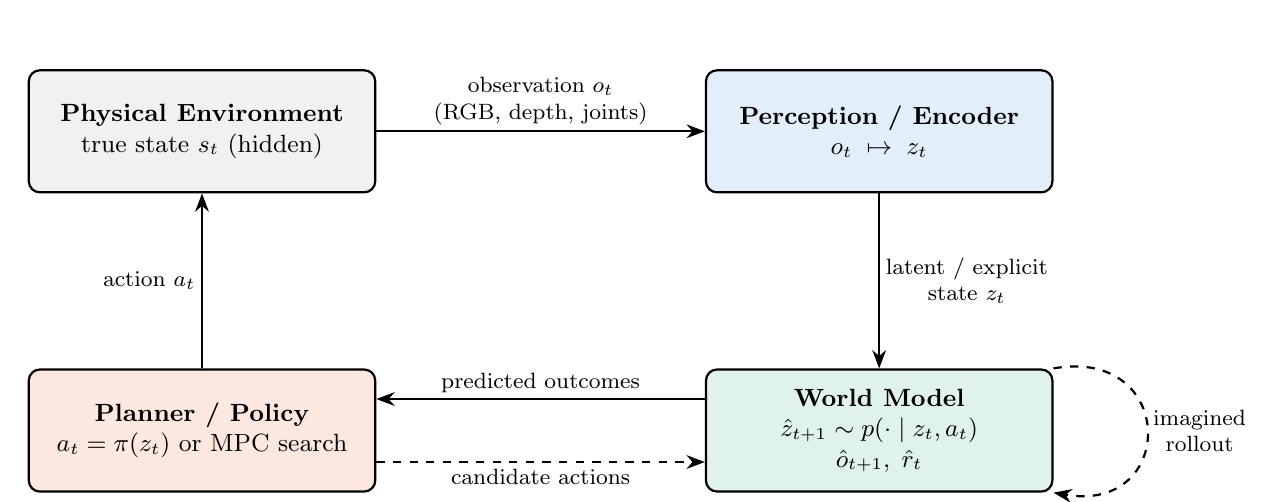
\begin{tikzpicture}[
  >=Stealth, thick,
  blk/.style={draw, rounded corners=4pt, align=center, minimum width=4.4cm, minimum height=1.55cm, font=\small},
  lbl/.style={font=\footnotesize, align=center, inner sep=2pt}]
\node[blk, fill=boxgray]   (env) at (0,0)    {\textbf{Physical Environment}\\ true state $s_t$ (hidden)};
\node[blk, fill=boxblue]   (enc) at (8.6,0)    {\textbf{Perception / Encoder}\\ $o_t \;\mapsto\; z_t$};
\node[blk, fill=boxgreen]  (wm)  at (8.6,-3.8) {\textbf{World Model}\\ $\hat{z}_{t+1}\sim p(\cdot\mid z_t,a_t)$\\ $\hat{o}_{t+1},\;\hat{r}_t$};
\node[blk, fill=boxorange] (pol) at (0,-3.8) {\textbf{Planner / Policy}\\ $a_t=\pi(z_t)$ or MPC search};
\draw[->] (env) -- node[lbl, above, text width=3.4cm]{observation $o_t$\\(RGB, depth, joints)} (enc);
\draw[->] (enc) -- node[lbl, right]{latent / explicit\\state $z_t$} (wm);
\draw[->] ([yshift=4mm]wm.west) -- node[lbl, above]{predicted outcomes} ([yshift=4mm]pol.east);
\draw[->, dashed] ([yshift=-4mm]pol.east) -- node[lbl, below]{candidate actions} ([yshift=-4mm]wm.west);
\draw[->] (pol) -- node[lbl, left]{action $a_t$} (env);
\draw[->, dashed] (wm.north east) to[out=10, in=-10, looseness=2.6] node[lbl, right]{imagined\\rollout} (wm.south east);
\end{tikzpicture}
\caption{The generic perception--prediction--action loop of a world-model-based agent. Candidate actions are evaluated inside the world model (dashed arrows) before a single action is sent to the real environment.}
\label{fig:wm_loop}
\end{figure}

\paragraph{} The four reviewed works instantiate the components of this loop very differently. In DexSim2Real$^2$, the ``state'' is an explicit URDF model loaded into the SAPIEN simulator and the transition model is the physics engine itself. In GAF, the state is a set of 3D Gaussians and the transition model is a learned per-Gaussian displacement field. In WMP, the state is the recurrent latent $h_t$ of an RSSM and the transition model is a GRU. In WMNav, the ``state'' is a Curiosity Value Map and the transition model is a VLM prompted to imagine what lies in each direction. This diversity is the central theme of the report.

\section{Latent World Models: The Recurrent State-Space Model}

\paragraph{} The Recurrent State-Space Model (RSSM), introduced in PlaNet and refined in the Dreamer series, is the most widely used latent world model. Its key insight is to split the latent state into a \emph{deterministic} recurrent component $h_t$, which carries information reliably over long horizons, and a \emph{stochastic} component $z_t$, which captures uncertainty and multi-modality. The model consists of
\begin{align}
\text{Recurrent model:}\quad & h_t = f_\phi(h_{t-1}, z_{t-1}, a_{t-1}), \\
\text{Encoder (posterior):}\quad & z_t \sim q_\phi(z_t \mid h_t, o_t), \\
\text{Dynamics predictor (prior):}\quad & \hat{z}_t \sim p_\phi(\hat{z}_t \mid h_t), \\
\text{Decoder:}\quad & \hat{o}_t \sim p_\phi(\hat{o}_t \mid h_t, z_t).
\end{align}
The recurrent model is typically a GRU. The posterior incorporates the current observation, while the prior must predict the stochastic state from history alone; at deployment, rolling the prior forward allows open-loop prediction of future observations.

\paragraph{} The RSSM is trained by maximizing a variational evidence lower bound (ELBO), which in practice becomes the minimization of a reconstruction loss plus a Kullback--Leibler (KL) regularizer over sequences of length $L$:
\begin{equation}
\mathcal{L}(\phi)=\mathbb{E}_{q_\phi}\Big[\sum_{t=1}^{L} -\ln p_\phi(o_t\mid h_t,z_t) \;+\; \beta\,\mathrm{KL}\big(q_\phi(z_t\mid h_t,o_t)\;\|\;p_\phi(z_t\mid h_t)\big)\Big].
\label{eq:rssm_loss}
\end{equation}
The reconstruction term forces the latent state to retain information about the observation, and the KL term makes the prior predictive of the posterior, so that the model can ``imagine'' without observations. Figure~\ref{fig:rssm} shows the RSSM unrolled in time with the reduced update frequency used by WMP.

\begin{figure}[htbp]
\centering
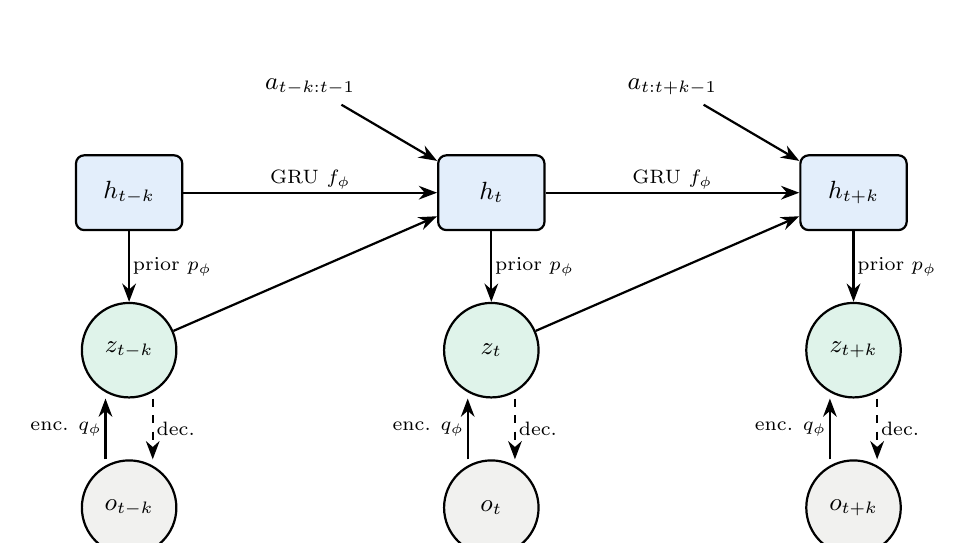
\begin{tikzpicture}[>=Stealth, thick,
 det/.style={draw, rectangle, rounded corners=3pt, minimum width=1.35cm, minimum height=0.95cm, fill=boxblue, font=\small},
 sto/.style={draw, circle, minimum size=1.2cm, fill=boxgreen, font=\small, inner sep=1pt},
 obs/.style={draw, circle, minimum size=1.2cm, fill=boxgray, font=\small, inner sep=1pt},
 lab/.style={font=\scriptsize, inner sep=1pt}]
\node[det] (h0) at (0,0)     {$h_{t-k}$};
\node[det] (h1) at (4.6,0)   {$h_{t}$};
\node[det] (h2) at (9.2,0)   {$h_{t+k}$};
\node[sto] (z0) at (0,-2)    {$z_{t-k}$};
\node[sto] (z1) at (4.6,-2)  {$z_{t}$};
\node[sto] (z2) at (9.2,-2)  {$z_{t+k}$};
\node[obs] (o0) at (0,-4)    {$o_{t-k}$};
\node[obs] (o1) at (4.6,-4)  {$o_{t}$};
\node[obs] (o2) at (9.2,-4)  {$o_{t+k}$};
\node[font=\small] (a0) at (2.3,1.35) {$a_{t-k:t-1}$};
\node[font=\small] (a1) at (6.9,1.35) {$a_{t:t+k-1}$};
\draw[->] (h0) -- node[lab, above]{GRU $f_\phi$} (h1);
\draw[->] (h1) -- node[lab, above]{GRU $f_\phi$} (h2);
\draw[->] (z0) -- (h1);
\draw[->] (z1) -- (h2);
\draw[->] (a0) -- (h1);
\draw[->] (a1) -- (h2);
\foreach \i in {0,1,2} {
  \draw[->] (h\i) -- node[lab, right]{prior $p_\phi$} (z\i);
  \draw[->] ([xshift=-3mm]o\i.north) -- node[lab, left]{enc. $q_\phi$} ([xshift=-3mm]z\i.south);
  \draw[->, dashed] ([xshift=3mm]z\i.south) -- node[lab, right]{dec.} ([xshift=3mm]o\i.north);
}
\end{tikzpicture}
\caption{The Recurrent State-Space Model unrolled over time. Rectangles are deterministic recurrent states, green circles stochastic latent states, and grey circles observations. In WMP the recurrent state is updated only every $k$ control steps using the accumulated action sequence.}
\label{fig:rssm}
\end{figure}

\section{Planning with World Models: Sampling-Based MPC}

\paragraph{} \textbf{Model Predictive Control} (MPC) uses a world model to repeatedly solve a finite-horizon optimization problem and executes only the first action of the resulting plan before re-planning. At time $t$ with planning horizon $h$, MPC solves
\begin{equation}
a^{*}_{t:t+h-1}=\arg\max_{a_{t:t+h-1}}\;\sum_{\tau=t}^{t+h-1} r(\hat{s}_\tau,a_\tau),\qquad \hat{s}_{\tau+1}=f(\hat{s}_\tau,a_\tau),\;\hat{s}_t=s_t,
\label{eq:mpc}
\end{equation}
where $f$ is the world model. When the model is a physics simulator with complex contacts, as in DexSim2Real$^2$, gradients of the objective are unavailable or uninformative, so \textbf{zeroth-order} (sampling-based) optimizers are used. The best known are the Covariance Matrix Adaptation Evolution Strategy (CMA-ES), the \textbf{Cross-Entropy Method} (CEM), and Model Predictive Path Integral control (MPPI).

\paragraph{} CEM maintains a Gaussian distribution $\mathcal{N}(\mu,\operatorname{diag}(\sigma^2))$ over action sequences. In each iteration it samples a population of $N$ sequences, evaluates each by rolling it out in the model, selects the $E$ highest-scoring sequences (the \emph{elite set}), and refits the distribution to the elites:
\begin{equation}
\mu \leftarrow \frac{1}{E}\sum_{e\in\mathcal{E}} A^{(e)},\qquad \sigma^{2}\leftarrow\frac{1}{E}\sum_{e\in\mathcal{E}}\big(A^{(e)}-\mu\big)^{2}.
\label{eq:cem}
\end{equation}
MPPI instead updates the mean with an exponentially weighted average of \emph{all} samples, $\mu \leftarrow \sum_n w_n A^{(n)}$ with $w_n \propto \exp\!\big(R^{(n)}/\lambda\big)$, where $\lambda$ is a temperature. The \textbf{improved CEM} (iCEM) \cite{icem} used by DexSim2Real$^2$ adds several refinements that reduce the number of samples needed for real-time planning: temporally correlated (coloured-noise) sampling that produces smoother action sequences, keeping a fraction of elites between iterations and between time steps, shifting the previous solution to initialize the next step, and executing the best sampled action rather than the mean. Algorithm~\ref{alg:cem} summarizes sampling-based MPC.

\begin{algorithm}[htbp]
\caption{Sampling-based MPC with the (improved) Cross-Entropy Method}\label{alg:cem}
\begin{algorithmic}[1]
\Require world model $f$, reward $r$, horizon $h$, population $N$, elite size $E$, iterations $I$, trajectory length $T$
\State Initialise mean $\mu_{0:h-1}\gets 0$ and standard deviation $\sigma_{0:h-1}$
\For{$t = 0,\dots,T-1$}
  \For{$i = 1,\dots,I$}
     \State Sample $N$ action sequences $A^{(n)}\sim\mathcal{N}(\mu,\operatorname{diag}(\sigma^2))$ \Comment{coloured noise in iCEM}
     \State Roll out each $A^{(n)}$ in the world model from $s_t$; compute $R^{(n)}=\sum_{\tau}r(\hat{s}_\tau,a^{(n)}_\tau)$
     \State Select the $E$ sequences with the highest $R^{(n)}$ as elite set $\mathcal{E}$ \Comment{reuse elites in iCEM}
     \State Refit $\mu,\sigma$ to $\mathcal{E}$ using Eq.~(\ref{eq:cem})
  \EndFor
  \State Apply the first action of the best sequence, observe $s_{t+1}$
  \State Shift $\mu$ by one step to warm-start the next optimisation
\EndFor
\State \Return executed trajectory $a_{0:T-1}$
\end{algorithmic}
\end{algorithm}

\paragraph{} The computational cost of sampling-based MPC grows with the dimension of the action space, because the number of samples needed to cover the space grows rapidly with dimension. This is why DexSim2Real$^2$ employs \textbf{eigengrasps}: Principal Component Analysis (PCA) is applied to a large dataset of hand postures, and the hand configuration is expressed as a linear combination of the first $m$ principal components,
\begin{equation}
q_h = \bar{q}_h + \sum_{i=1}^{m} \alpha_i\, e_i, \qquad m \ll d_{\mathrm{hand}},
\label{eq:eigen_general}
\end{equation}
where $e_i$ are the eigenvectors with the largest eigenvalues and $\alpha_i$ are the low-dimensional coefficients searched by the planner. Because human and robot grasps are highly correlated across joints, a handful of components captures most of the variance of natural hand postures.

\section{Explicit Scene Representations: 3D Gaussian Splatting}

\paragraph{} \textbf{3D Gaussian Splatting} (3DGS) \cite{kerbl2023} represents a scene as a set of anisotropic 3D Gaussians, each with a centre $\mu\in\mathbb{R}^3$, a covariance $\Sigma$, an opacity $\sigma$, and a colour $c$ (often represented with spherical harmonics). The density of a Gaussian at point $x$ is
\begin{equation}
G(x)=\exp\!\Big(-\tfrac{1}{2}(x-\mu)^{\top}\Sigma^{-1}(x-\mu)\Big),\qquad \Sigma = R\,S\,S^{\top}R^{\top},
\label{eq:gauss}
\end{equation}
where the covariance is factorized into a rotation $R$ (stored as a quaternion $r$) and a diagonal scale matrix $S$ (stored as a vector $s$) to guarantee positive semi-definiteness. To render an image, each Gaussian is projected to the image plane with covariance $\Sigma' = J W \Sigma W^{\top} J^{\top}$, where $W$ is the viewing transformation and $J$ the Jacobian of the projective transformation, and the pixel colour is obtained by front-to-back alpha blending of the $N$ depth-sorted Gaussians that overlap the pixel:
\begin{equation}
C(p)=\sum_{i=1}^{N} c_i\,\alpha_i \prod_{j=1}^{i-1}(1-\alpha_j),\qquad \alpha_i=\sigma_i\, e^{-\frac{1}{2}(p-\mu^{2d}_i)^{\top}{\Sigma'_i}^{-1}(p-\mu^{2d}_i)}.
\label{eq:alphablend}
\end{equation}
Because this rasterization is differentiable, the Gaussian parameters can be optimized directly from multi-view images using photometric losses, without any 3D ground truth. Compared with Neural Radiance Fields, which query a neural network at many points along each camera ray, 3DGS renders in real time and provides an explicit point-based geometry that can be manipulated, segmented, and registered. These properties make it attractive as a world representation for robotics: GAF \cite{p2} extends each Gaussian with a motion vector $\Delta\mu$ so that the same representation also encodes how the scene will change.

\section{Diffusion Models for Action Generation}

\paragraph{} \textbf{Denoising diffusion probabilistic models} (DDPMs) learn to generate data by reversing a gradual noising process. The forward process corrupts a clean sample $x_0$ into $x_k$ according to
\begin{equation}
q(x_k\mid x_0)=\mathcal{N}\big(\sqrt{\bar{\alpha}_k}\,x_0,\;(1-\bar{\alpha}_k)\,I\big),
\end{equation}
where $\bar{\alpha}_k$ follows a fixed noise schedule. A network $\epsilon_\theta$ is trained to predict the injected noise, $\mathcal{L}=\mathbb{E}_{x_0,\epsilon,k}\big[\|\epsilon-\epsilon_\theta(x_k,k)\|^2\big]$, and new samples are generated by iteratively denoising pure Gaussian noise. \textbf{Denoising Diffusion Implicit Models} (DDIM) define a non-Markovian sampling process that produces high-quality samples in far fewer steps.

\paragraph{} In robotics, \textbf{Diffusion Policy} applies this machinery to action sequences: the ``data'' $x_0$ is a short sequence of future end-effector poses, and the denoiser is conditioned on the current observation. Diffusion policies naturally represent multi-modal action distributions (for example, going around an obstacle on either side), which is difficult for regression-based policies. GAF uses a diffusion model conditioned on renderings of candidate gripper poses (following Render-and-Diffuse) to refine its initial action estimate, and at inference time it needs only three DDIM iterations.

\section{Foundation Models as World Knowledge}

\paragraph{} \textbf{Large Language Models} (LLMs) are trained on internet-scale text and encode a large amount of commonsense knowledge about the world---for example, that beds are usually found in bedrooms, that bedrooms are often off a hallway, and that refrigerators are in kitchens. \textbf{Vision-Language Models} (VLMs) extend this capability to images by aligning visual features with language, either through contrastive embedding models or through generative multimodal models that can answer free-form questions about an image. Recent work has therefore asked whether such models can act as \emph{abstract world models}: rather than simulating physics, they predict the likely outcome of a decision at a semantic level (``if I go through that door, I will probably find a bedroom'').

\paragraph{} Foundation models offer three advantages for embodied world modeling: zero-shot generalization to new object categories and environments, no task-specific training data, and the ability to explain their predictions in natural language. They also have well-known weaknesses. They may \textbf{hallucinate}---confidently describing objects or relations that are not present---they are relatively slow and expensive to query, and they struggle with precise metric reasoning such as estimating distances in pixels. WMNav's design choices (quantitative scoring, subtask feedback, and a two-stage action proposer) are directly aimed at these weaknesses.

\section{Sim-to-Real Transfer}

\paragraph{} Training in simulation is fast, safe, and cheap, but policies and models trained in simulation must ultimately operate on real hardware. The \textbf{sim-to-real gap} arises from unmodeled dynamics (friction, compliance, actuator delays), sensor differences (noise and artifacts in real depth images), and visual appearance. Several techniques are used to bridge it:
\begin{itemize}
  \item \textbf{Domain randomization}: physical parameters (mass, friction, motor strength) and sensor properties are randomized during training so that the real world appears as just another sample from the training distribution.
  \item \textbf{Latency and noise modelling}: sensing and computation delays are simulated explicitly; for example, WMP delivers depth images to the policy with a 100 ms delay in simulation.
  \item \textbf{Privileged learning}: a teacher policy with access to ground-truth simulator information is trained first, and a student policy that sees only onboard sensors is trained to imitate it.
  \item \textbf{Asymmetric actor--critic}: the critic receives privileged information during training, while the actor uses only deployable observations.
  \item \textbf{Real-to-sim-to-real}: a digital twin of the real object or scene is reconstructed, behaviors are planned or learned on the twin, and the result is executed on the real system. This is the strategy of DexSim2Real$^2$.
\end{itemize}

\section{Evaluation Metrics}

\paragraph{} Because the reviewed works target different tasks, they are evaluated with different metrics. The most important are summarized below; they are referred to throughout Chapters 3 and 4.

\paragraph{} \textbf{Manipulation error.} For goal-conditioned articulated manipulation, the real joint movement $\Delta s_{\mathrm{real}}=s_{\mathrm{real}}-s_{\mathrm{initial}}$ is compared with the target movement $\Delta s_{\mathrm{target}}=s_{\mathrm{target}}-s_{\mathrm{initial}}$, giving an absolute error $\delta=\Delta s_{\mathrm{real}}-\Delta s_{\mathrm{target}}$ (in degrees or centimetres) and a relative error $\delta_r=\delta/\Delta s_{\mathrm{target}}\times100\%$ \cite{p1}.

\paragraph{} \textbf{Success rate.} The fraction of trials that complete the task, used for RLBench manipulation, real-robot tasks, and legged traversal of obstacles of increasing difficulty.

\paragraph{} \textbf{Reconstruction quality.} The Peak Signal-to-Noise Ratio (PSNR), computed as $10\log_{10}(\mathrm{MAX}^2/\mathrm{MSE})$ decibels, measures photometric fidelity; the Structural Similarity Index (SSIM) measures structural agreement; and the Learned Perceptual Image Patch Similarity (LPIPS) measures perceptual distance using deep features (lower is better).

\paragraph{} \textbf{Locomotion metrics.} The average RL return, and the velocity tracking error, defined as the mean squared error between the commanded planar velocity $v^{\mathrm{cmd}}_{xy}$ and the achieved velocity $v_{xy}$ \cite{p3}.

\paragraph{} \textbf{Navigation metrics.} Success Rate (SR) and Success weighted by (normalized inverse) Path Length (SPL):
\begin{equation}
\mathrm{SPL}=\frac{1}{N}\sum_{i=1}^{N} S_i\,\frac{\ell_i}{\max(p_i,\ell_i)},
\label{eq:spl}
\end{equation}
where $S_i\in\{0,1\}$ indicates success in episode $i$, $\ell_i$ is the shortest-path distance from start to goal, and $p_i$ is the length of the path actually taken. SPL rewards agents that not only succeed but do so efficiently.

\section{Taxonomy of World Models in Embodied AI}

\paragraph{} Combining the concepts above, world models used in embodied AI can be organized into four families according to how they represent the world and how they are used for control. Figure~\ref{fig:taxonomy_wm} places the four reviewed works in this taxonomy, and Table~\ref{tab:taxonomy} summarizes the defining characteristics of each family.

\begin{figure}[htbp]
   \centering
   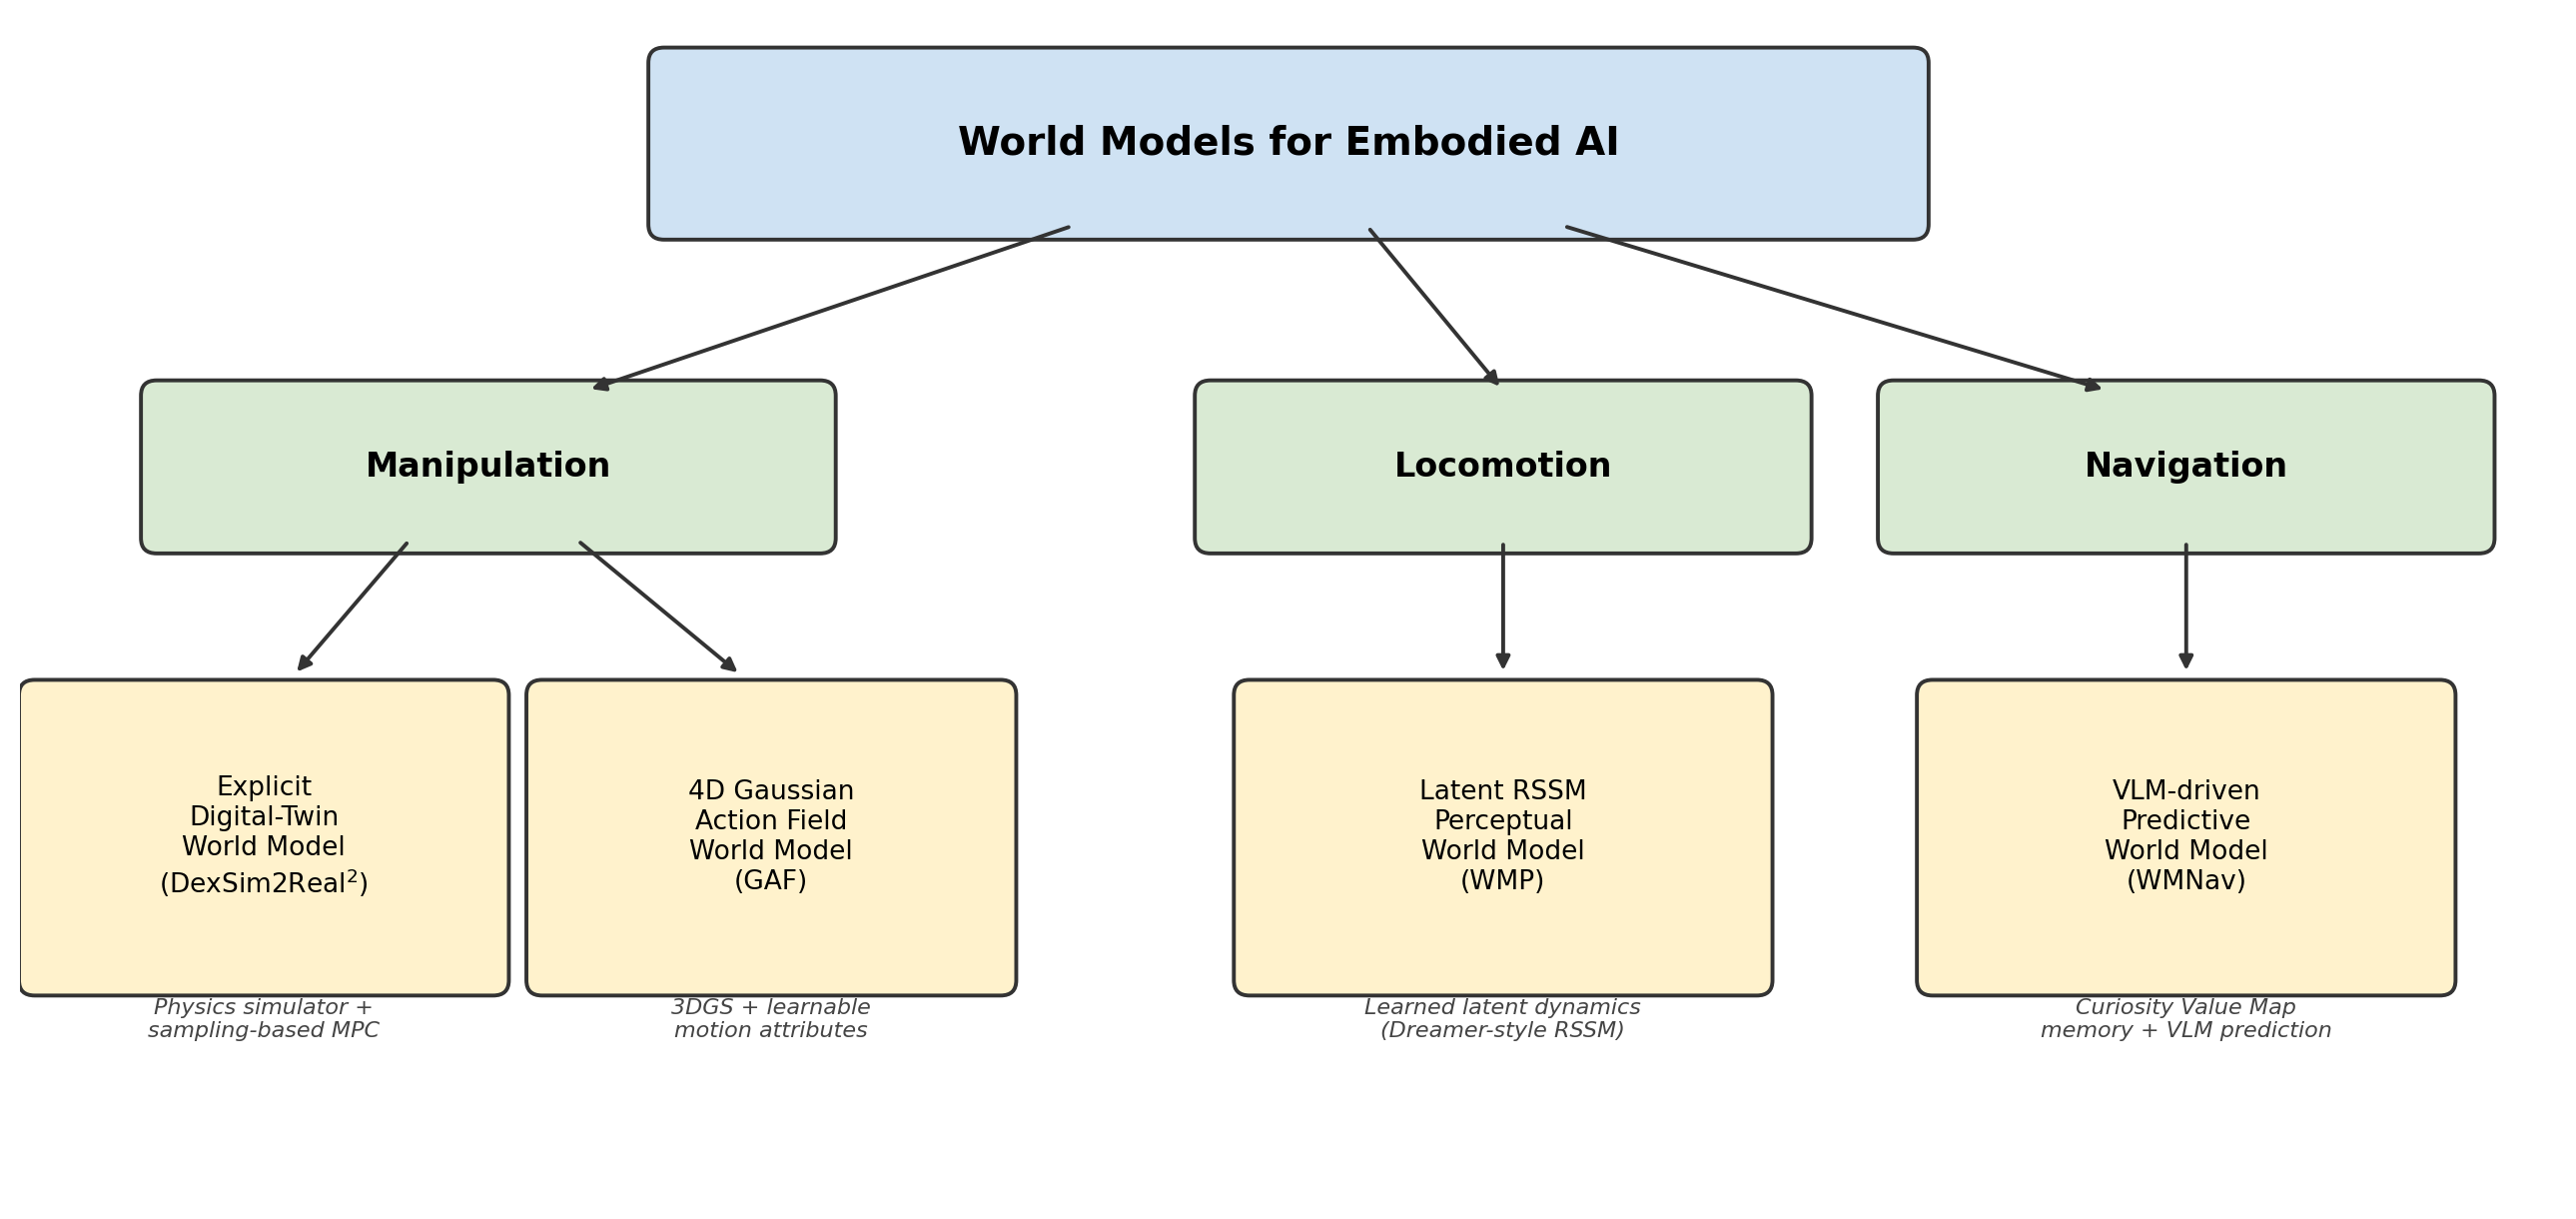
\includegraphics[width=0.9\linewidth,height=.32\textheight,keepaspectratio]{taxonomy.png}
   \caption{Taxonomy of world-model approaches in embodied AI}
   \label{fig:taxonomy_wm}
\end{figure}

{\renewcommand{\arraystretch}{1.2}
\begin{table}[htbp]
\centering
\caption{Families of world models and their characteristics}\label{tab:taxonomy}
\small
\begin{tabularx}{\textwidth}{|p{2.7cm}|X|X|p{2.6cm}|}
\hline
\textbf{Family} & \textbf{Representation} & \textbf{Typical use} & \textbf{Reviewed work} \\ \hline
Explicit physics-based & Digital twin (meshes, joints, URDF) in a physics engine & Sampling-based MPC, trajectory search, tool use & DexSim2Real$^2$ \cite{p1} \\ \hline
Explicit geometric (4D) & 3D Gaussians with motion attributes & Future-scene prediction, action extraction and refinement & GAF \cite{p2} \\ \hline
Latent (learned) & Recurrent deterministic + stochastic latent state (RSSM) & Perception for a learned policy, imagination-based RL & WMP \cite{p3} \\ \hline
Semantic / foundation-model & Language-grounded predictions stored in a value map & Zero-shot high-level planning and exploration & WMNav \cite{p4} \\ \hline
\end{tabularx}
\end{table}}

\section{Chapter Summary}

\paragraph{} This chapter introduced the concepts needed to understand the four reviewed systems. Embodied control was formulated as a POMDP, in which the agent must act on partial observations and therefore benefits from an internal model that summarizes history and predicts the future. World models were defined through their representation, transition, observation, and reward components, and the two main ways of using them---planning at decision time and learning policies from predicted experience---were contrasted. The remaining sections described the specific tools on which each reviewed paper builds:
\begin{itemize}
  \item \textbf{POMDPs, PPO, and the RSSM} provide the formulation, the policy optimizer, and the latent world model of WMP \cite{p3}.
  \item \textbf{Sampling-based MPC, iCEM, and eigengrasps} provide the planner and the action-space reduction of DexSim2Real$^2$ \cite{p1}.
  \item \textbf{3D Gaussian Splatting and diffusion models} provide the scene representation and the action refinement of GAF \cite{p2}.
  \item \textbf{Foundation models} provide the commonsense predictor at the heart of WMNav \cite{p4}.
  \item \textbf{Sim-to-real techniques and metrics} explain how the systems are validated.
\end{itemize}


% -----------------------------
% CHAPTER 3: LITERATURE SURVEY
% -----------------------------
\chapter{Literature Survey}

\paragraph{}
This chapter reviews four selected research papers under the theme of \textbf{World Models for Embodied AI}.
Each work instantiates the world-model paradigm in a different embodied domain and with a different representation: an explicit digital-twin world model for precise articulated object manipulation, a 4D Gaussian Action Field for dynamic manipulation scenes, a latent recurrent world model for visual legged locomotion, and a VLM-driven predictive world model for zero-shot object goal navigation.
Together, these studies illustrate the evolution of embodied agents from reactive perception--action mappings toward predictive, simulation-capable intelligence. For each paper, the problem setting, architecture, key equations, experimental protocol, and principal results are presented, followed by a short critical discussion.

%---------------------------------------------------------------

\section{DexSim2Real$^2$: Building Explicit World Model for Precise Articulated Object Dexterous Manipulation}

This paper, the base paper of the seminar, proposes a robot learning framework for precise, goal-conditioned manipulation of unseen articulated objects using suction grippers, two-finger grippers, and multi-finger dexterous hands \cite{p1}. Its core idea is to use a physics simulator as the robot's ``mental model'': the robot first interacts with the object to reveal its structure, then constructs an explicit digital twin of the object in simulation, and finally plans long-horizon manipulation trajectories inside this world model using sampling-based Model Predictive Control (MPC), without demonstrations or reinforcement learning. The work extends the authors' earlier ICRA paper Sim2Real$^2$.

\subsection{Problem Statement and Motivation}

\paragraph{} Articulated objects---drawers, cabinets, laptops, lamps, refrigerators---are ubiquitous in daily life, and manipulating them is considerably harder than pick-and-place. In pick-and-place only the start and end poses of the end effector are constrained, whereas articulated object manipulation requires the end effector to follow a trajectory dictated by the object's kinematic constraint. Most existing approaches train a neural network with RL or IL to map object states to actions, but the state distribution of articulated objects is high-dimensional and complex, so such networks struggle to learn the correlation even with hundreds of demonstrations and millions of interactions. Methods such as FlowBot and UMPNet predict one-step actions from a single frame and are tied to suction grippers.

\paragraph{} DexSim2Real$^2$ addresses the \emph{goal-conditioned} version of the problem: given an unseen articulated object and a target joint state $s_{\mathrm{target}}$, drive the object precisely to that state with any of several end effectors. The key observation is that a single view of an object cannot reveal its full structure---it is hard to tell from one look whether a kitchen door has a rotating or a sliding hinge---but after the door is moved slightly, the two observations together make the structure obvious. The framework therefore separates the problem into a \emph{generalizable} part (predicting a simple interaction and building a model) and an \emph{instance-specific} part (planning with the model of the one object in front of the robot).

\subsection{Framework Overview}

\paragraph{} As shown in Figure~\ref{fig:paper1_wm}, the framework consists of three phases. (1) In \textbf{Interactive Perception}, an affordance prediction module proposes a one-step interaction from a partial point cloud of the object; the robot executes it to change the object's joint state and captures new observations, repeating this $K$ times for an object with $K$ movable parts. (2) In \textbf{Explicit World Model Construction}, the $K+1$ frames of observations are used to build a digital twin---part meshes plus kinematic structure---that can be loaded into a physics simulator. (3) In \textbf{Sampling-based Model Predictive Control}, a long-horizon trajectory is searched in simulation and then executed on the real robot; for dexterous hands, an eigengrasp module first reduces the action dimension.

\begin{figure}[htbp]
   \centering
   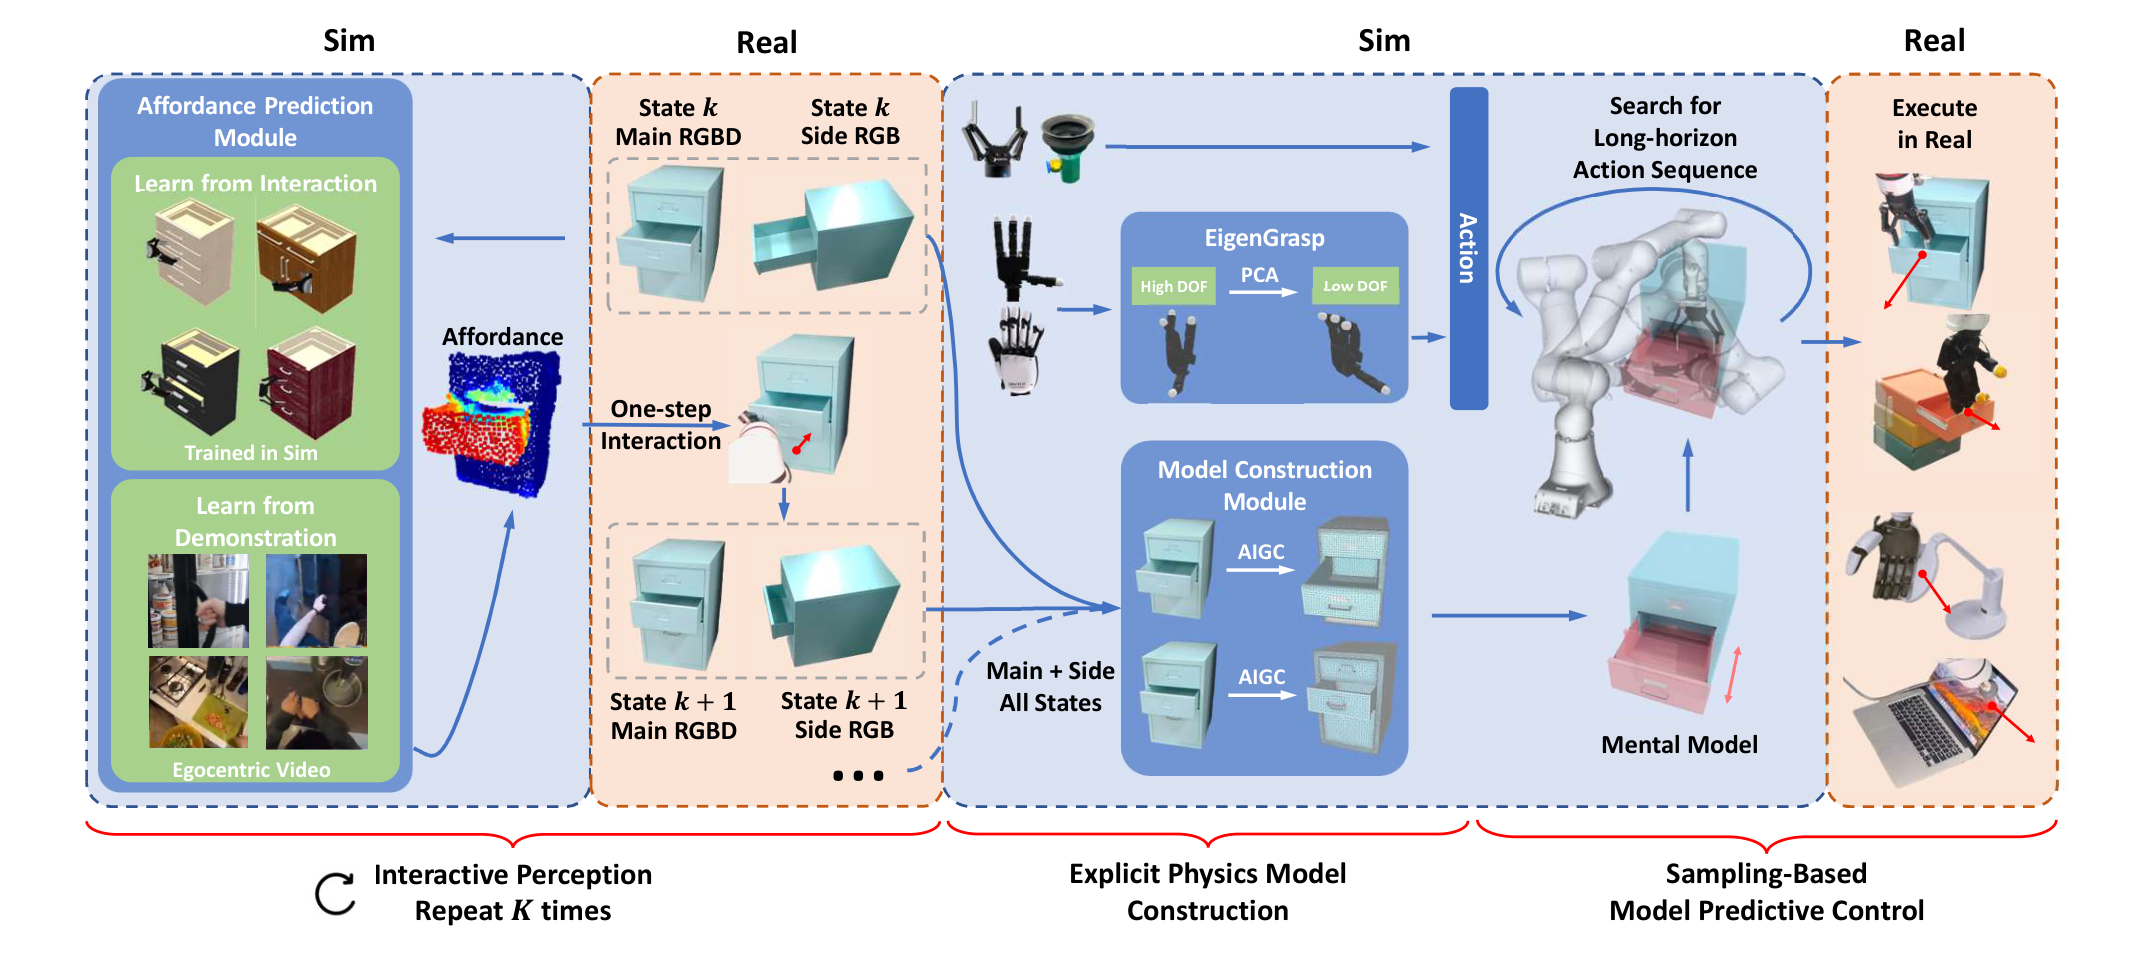
\includegraphics[width=0.92\linewidth,height=.27\textheight,keepaspectratio]{dexsim_framework.png}
   \caption{Overview of the DexSim2Real$^2$ framework \cite{p1}}
   \label{fig:paper1_wm}
\end{figure}

\subsection{Interactive Perception}

\paragraph{} The purpose of interactive perception is only to \emph{change} the state of each movable part; the interaction does not need to be precise. Affordance estimation depends only on the object and therefore generalizes better to novel objects than a full manipulation policy. Two sources of affordance knowledge are studied.

\paragraph{} \textbf{Learning from self-supervised interaction in simulation.} The framework uses Where2Act, which contains an Actionability Scoring Module that predicts a per-point score $a_p$ (the likelihood that acting at that point moves a part), an Action Proposal Module that proposes gripper poses for a point, and an Action Scoring Module that predicts the success likelihood of each proposal. Because Where2Act assumes a free-flying gripper and ignores the robot's kinematics, many top-scoring proposals are unreachable. DexSim2Real$^2$ therefore selects the $n_p$ points with the highest actionability, keeps the $n_a$ best actions for each, and attempts motion planning sequentially until a feasible action is found ($n_p=n_a=10$ in the experiments).

\paragraph{} \textbf{Learning from real-world egocentric human videos.} Simulation-based affordance learning requires interactable 3D assets, which are scarce. The authors therefore also use the Vision-Robotics Bridge (VRB), trained on videos of humans manipulating objects, which predicts a 2D contact heatmap and a 2D post-contact trajectory vector in the image. To lift these 2D predictions into a 3D robot motion, a novel \textbf{pixel projection} method is proposed (Figure~\ref{fig:dex_aff}). Given the RGB image $I_0$, depth map $D_0$, camera intrinsics $K$ and extrinsics $H_0$, a virtual camera with pose $H$ is placed and a virtual image $\hat{I}_0$ is synthesized by image warping. VRB is run on both images, producing contact points $c_0=(u_0,v_0)$, $\hat{c}_0$ and post-contact vectors $\tau_0=(u_0'-u_0,\,v_0'-v_0)$, $\hat{\tau}_0$. The 3D contact point in the robot base frame is
\begin{equation}
p_c = H_0^{-1}K^{-1}z_c\,[u_0,\;v_0,\;1]^{\top},
\end{equation}
where $z_c$ is the depth of the contact point. Each 2D vector is the projection of infinitely many 3D vectors that lie in a common \emph{projection plane}. For the real camera this plane is spanned by
\begin{equation}
\varphi_0 = p_c' - p_c, \qquad \varphi_0' = p_c - o_{c_0}, \qquad p_c' = H_0^{-1}K^{-1}z_c\,[u_0',\;v_0',\;1]^{\top},
\end{equation}
where $o_{c_0}$ is the camera origin in the robot frame. The plane normal is $n_0=\varphi_0\times\varphi_0'$, the normal $\hat{n}_0$ of the virtual camera's plane is computed in the same way, and the 3D post-contact direction is the intersection of the two planes:
\begin{equation}
\tau_c = n_0 \times \hat{n}_0 .
\end{equation}
The robot then moves its end effector to $p_c$ and pushes a fixed distance along $\tau_c$. For fully closed cabinets and drawers where pushing is infeasible, VRB is used to detect the handle, the gripper is placed behind it, closed, and pulled along $\tau_c$. For objects with $K>1$ movable parts, affordance points are detected iteratively by masking the neighbourhood of each found point.

\begin{figure}[htbp]
   \centering
   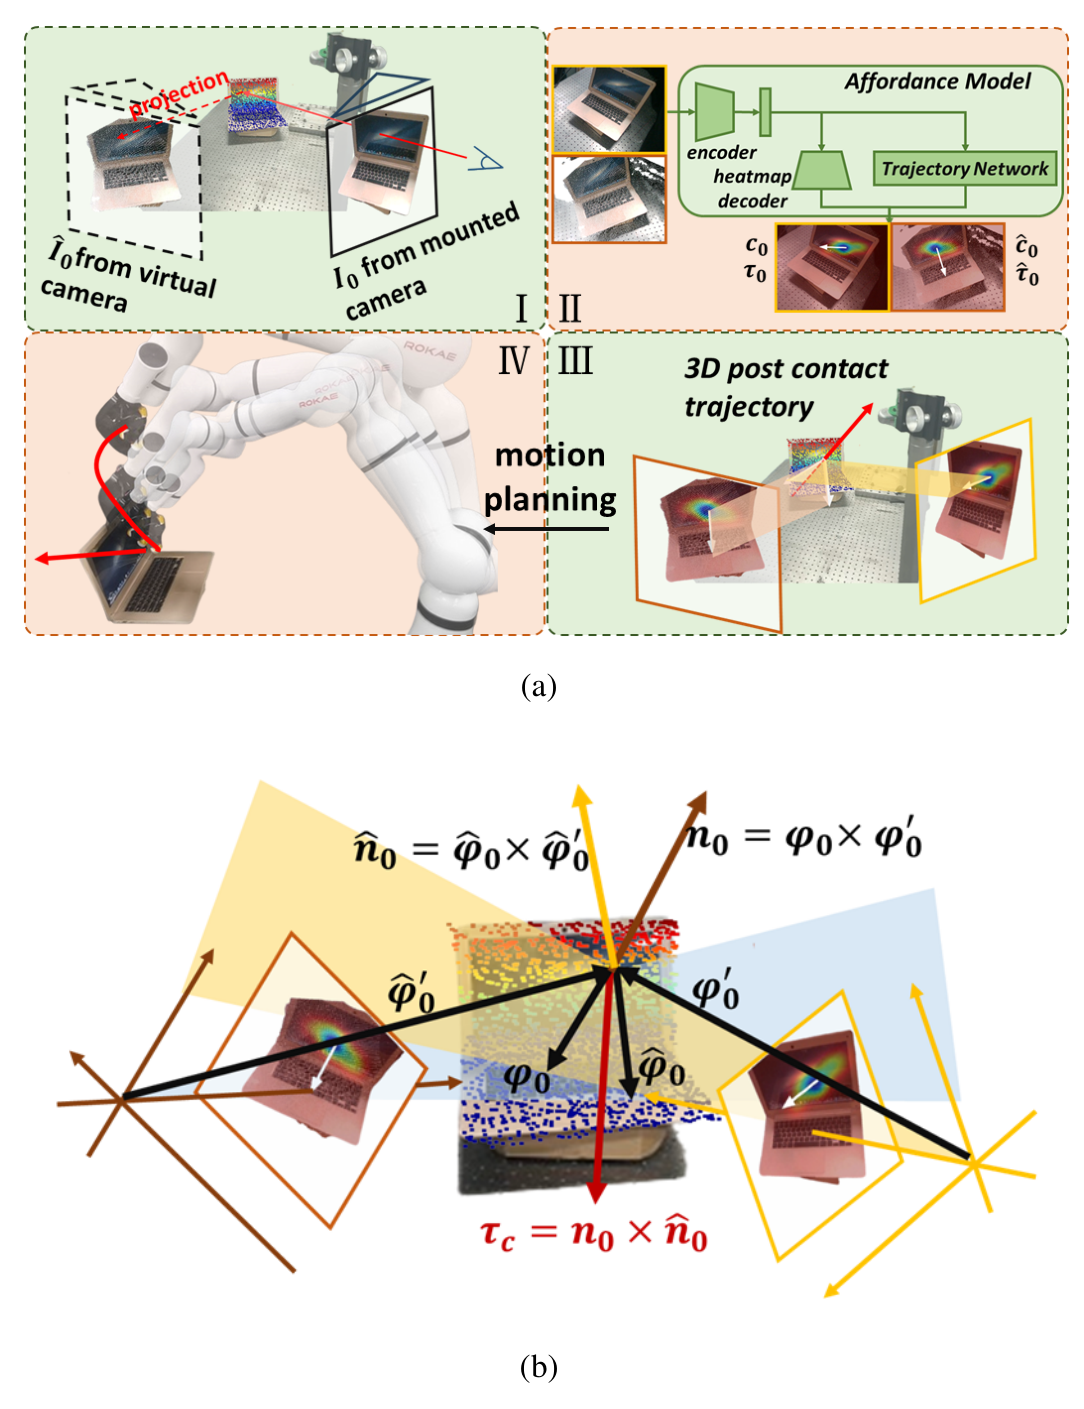
\includegraphics[width=0.48\linewidth,keepaspectratio]{figs/dex_affordance3d.png}
   \caption{(a) Generating a real robot manipulation trajectory from 2D affordances; (b) computing the 3D post-contact vector as the intersection of two projection planes \cite{p1}}
   \label{fig:dex_aff}
\end{figure}

\subsection{Explicit World Model Construction}

\paragraph{} The second module builds the digital twin from the $K+1$ observation frames
\begin{equation}
\big\{I_0^{(k)},\,D_0^{(k)},\,M_0^{(k)},\,I_1^{(k)},\,M_1^{(k)},\,\ldots,\,I_C^{(k)},\,M_C^{(k)}\big\}_{k=0}^{K},
\end{equation}
where $I_0, D_0$ come from the main RGB-D sensor, $I_c$ from $C$ additional uncalibrated RGB cameras ($C=1$ in the experiments), and $M$ are object masks. The pipeline, shown in Figure~\ref{fig:dex_model}, has four stages.

\begin{figure}[htbp]
   \centering
   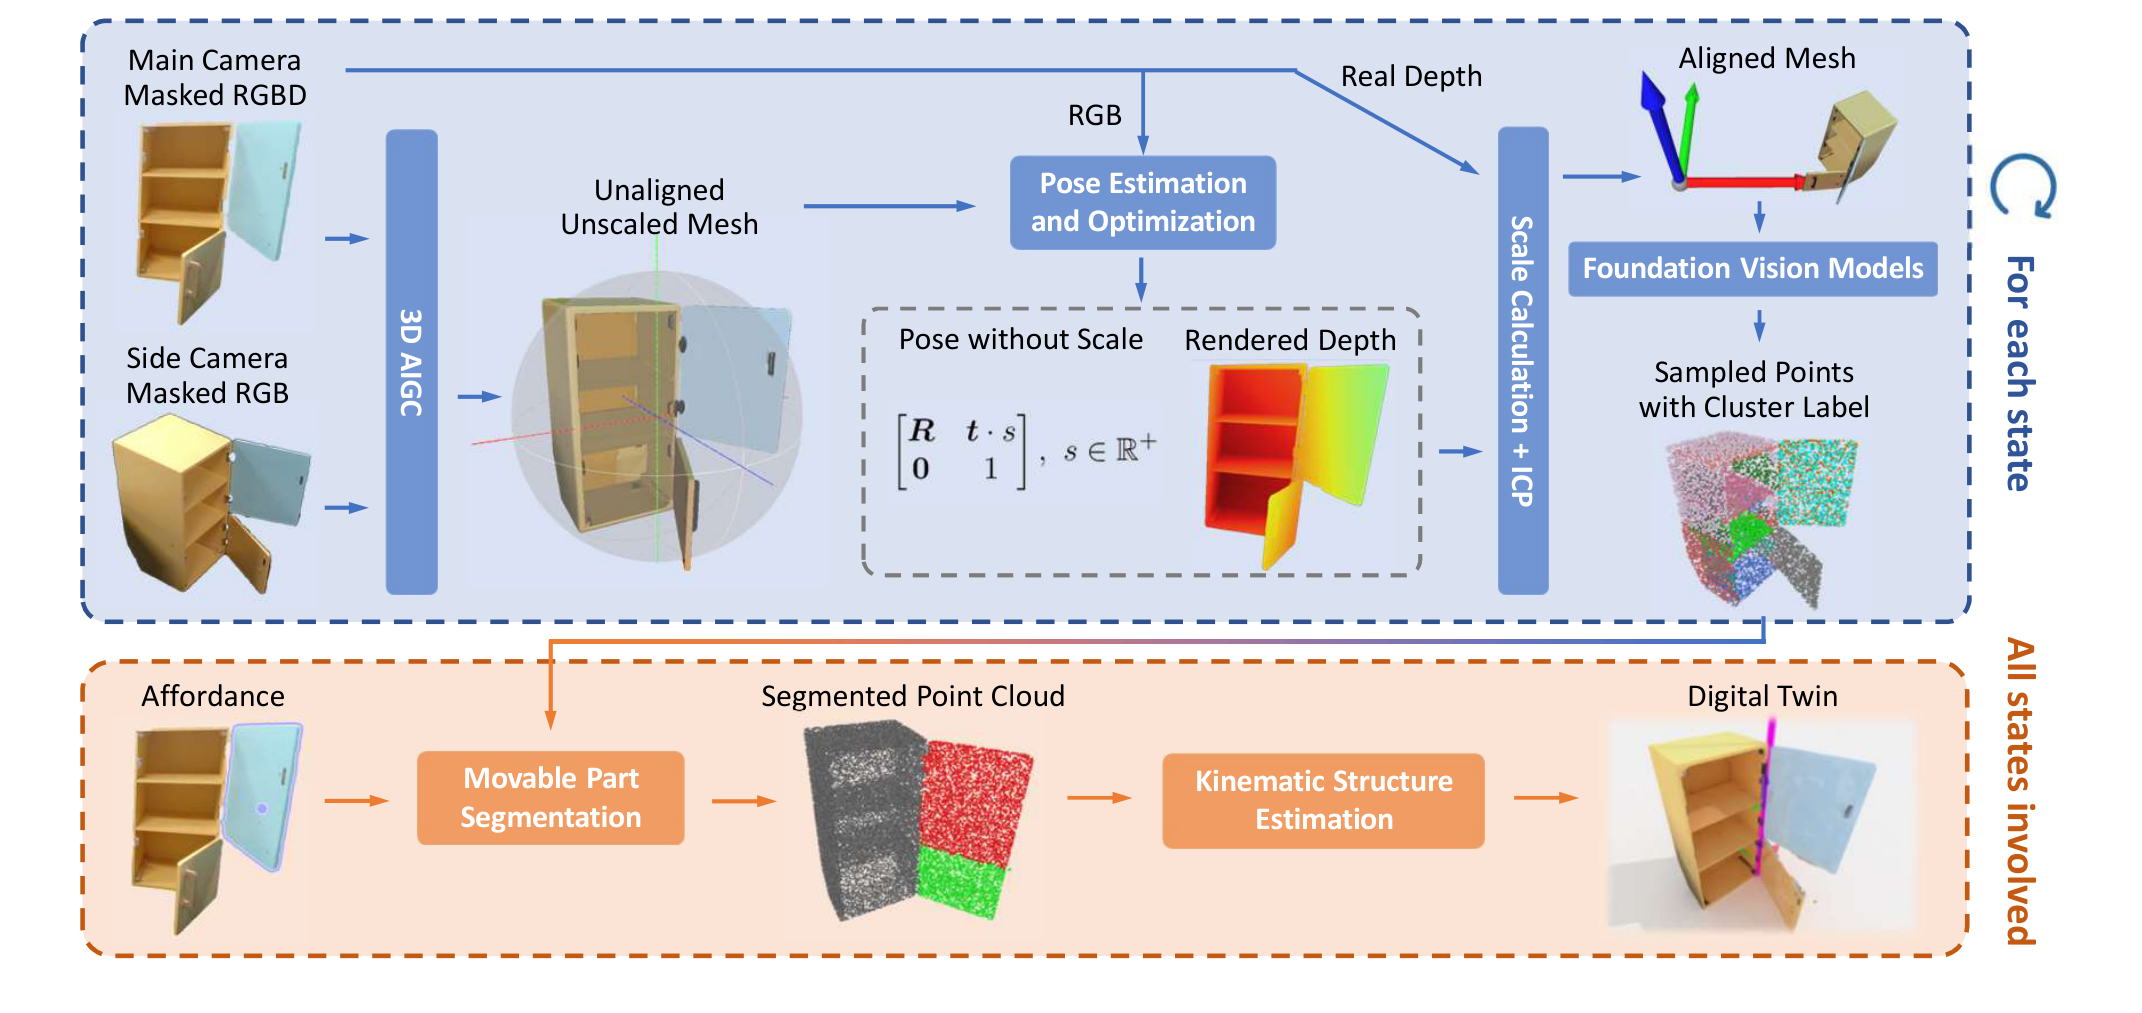
\includegraphics[width=0.92\linewidth,height=.27\textheight,keepaspectratio]{dexsim_modelconstruction.png}
   \caption{Explicit world model construction pipeline: 3D AIGC mesh generation, pose and scale estimation, movable part segmentation, and kinematic structure estimation \cite{p1}}
   \label{fig:dex_model}
\end{figure}

\paragraph{} \textbf{1) Canonical mesh generation.} For each state $k$, a controllable large-scale 3D generative model, Rodin, generates a textured canonical mesh $\tilde{A}^{(k)}$ conditioned on the masked multi-view images. Using 3D AIGC rather than direct depth fusion yields complete, high-quality geometry even for regions that are not visible from the main camera.

\paragraph{} \textbf{2) Mesh positioning and scaling.} The generated mesh is centred at the origin and normalized to unit size, so standard CAD-based pose estimators cannot be applied directly. The authors modify FoundationPose: images of $\tilde{A}^{(k)}$ are rendered under many pose hypotheses and ranked by similarity to $I_0^{(k)}$, and the best hypothesis is refined by aligning rendered edges to the mask $M_0^{(k)}$ using differentiable rendering, with the orientation constrained to rotate about the Z-axis for stability. Given the orientation and unscaled translation, an unscaled depth map $\tilde{D}_0^{(k)}$ is rendered and the metric scale is recovered as the ratio of real to rendered depth over the object mask:
\begin{equation}
s^{(k)}=\frac{\sum_{M_0^{(k)}} D_0^{(k)}}{\sum_{M_0^{(k)}} \tilde{D}_0^{(k)}}.
\end{equation}

\paragraph{} \textbf{3) Movable part segmentation.} Distinguishing parts from a single static mesh is difficult, so all $K+1$ meshes are used jointly. Each mesh is first split into small sub-parts using the foundation 3D segmentation model SAMPart3D. For each sub-part, bidirectional nearest-neighbour (chamfer-style) distances to the previous frame's point cloud are computed; a sub-part is considered moved if these distances are large or their distributions differ. To make this robust to inconsistencies of 3D AIGC and pose errors, two further cues are used: \emph{mesh connectivity}, encoded as a graph $G^{(k)}=\langle Q^{(k)},E^{(k)}\rangle$ over sub-parts, and \emph{robot proprioception}---the sub-part closest to the end effector during interaction must have moved. The graph is traversed breadth-first from this sub-part, and a sub-part is labelled as moved only if at least one predecessor is moved. Algorithm~\ref{alg:partseg} summarizes the procedure.

\begin{algorithm}[htbp]
\caption{Movable part segmentation in DexSim2Real$^2$ (adapted from \cite{p1})}\label{alg:partseg}
\begin{algorithmic}[1]
\Require meshes $\{A^{(k)}\}_{k=0}^{K}$
\Ensure movable part segmentation $S^{(K)}$
\For{$k=0,\dots,K$}
  \State Segment $A^{(k)}$ into sub-parts $Q^{(k)}$ with SAMPart3D
  \State Build graph $G^{(k)}=\langle Q^{(k)},E^{(k)}\rangle$; find sub-part $Q_{\mathrm{closest}}$ nearest the end effector
  \State Sample point cloud $P^{(k)}$ with sub-part indices from $A^{(k)}$
\EndFor
\State $S^{(0)}\gets 0$
\For{$k=1,\dots,K$}
  \For{each sub-part $Q$ in breadth-first order of $G^{(k)}$ from $Q_{\mathrm{closest}}$}
    \State $P\gets P^{(k)}[x]$ for the point indices $x$ of $Q$
    \State Compute distances $\{d_i^{(k)\to(k-1)}\}$ from $P$ to its closest points $P^B$ in $P^{(k-1)}$
    \State Compute distances $\{d_i^{(k-1)\to(k)}\}$ from $P^B$ back to $P^{(k)}$
    \If{distances indicate motion \textbf{and} a predecessor of $Q$ is moved}
      \State $S^{(k)}[x]\gets k$
    \Else
      \State $S^{(k)}[x]\gets S^{(k-1)}[x_{\mathrm{closest}}]$
    \EndIf
  \EndFor
\EndFor
\State \Return $S^{(K)}$
\end{algorithmic}
\end{algorithm}

\paragraph{} \textbf{4) Kinematic structure construction.} Finally, the part tree hierarchy, joint categories (prismatic or revolute), and joint configurations (axis direction and origin) are estimated following Liu et al.: per-part rigid transformations between frames are estimated and then projected onto a valid kinematic model. The result is exported in the Unified Robot Description Format (URDF), the meshes are convex-decomposed with VHACD for stable contact simulation, and the twin is loaded into the SAPIEN simulator. Compared with Ditto, this pipeline handles objects with more than one movable part and produces significantly higher-quality geometry.

\subsection{Sampling-Based MPC with Eigengrasp}

\paragraph{} With the digital twin in hand, the agent must find a trajectory that changes the joint state from $s_{\mathrm{initial}}$ to $s_{\mathrm{target}}$, i.e.\ achieve $\Delta s_{\mathrm{target}}=s_{\mathrm{target}}-s_{\mathrm{initial}}$. Because contacts between the end effector and the object make the objective non-smooth, the zeroth-order iCEM planner (Section 2.5) is used. At each time step $t<T$ the action $a_t\in\mathbb{R}^{d}$ is an increment of the robot's joint positions, where $d=7$ for the suction gripper (7-DOF arm), $d=8$ for the two-finger gripper (arm plus gripper), and $d=7+d_{\mathrm{hand}}$ for a dexterous hand. The population, planning horizon $h$, and elite set size $E$ control the search.

\paragraph{} For dexterous hands, searching directly in the $7+16=23$-dimensional space of the Allegro Hand is computationally prohibitive and produces unnatural postures. The authors therefore generate a dataset of grasp postures with DexGraspNet---60{,}800 grasps across 474 objects for the Allegro Hand and the XHand---perform PCA, and keep the first $m$ eigenvectors $e_1,\ldots,e_m$. iCEM then searches over $a_t\in\mathbb{R}^{7+m}$ and the hand joint angles are recovered as
\begin{equation}
q_h=\sum_{i=1}^{m} a_i\, e_i .
\end{equation}
Figure~\ref{fig:dex_eigen} shows that the accumulated variance ratio of the two hands follows nearly the same curve despite their different numbers of joints, suggesting that eigengrasps capture fundamental features of hand posture; $m=2$ is used unless stated otherwise.

\begin{figure}[htbp]
   \centering
   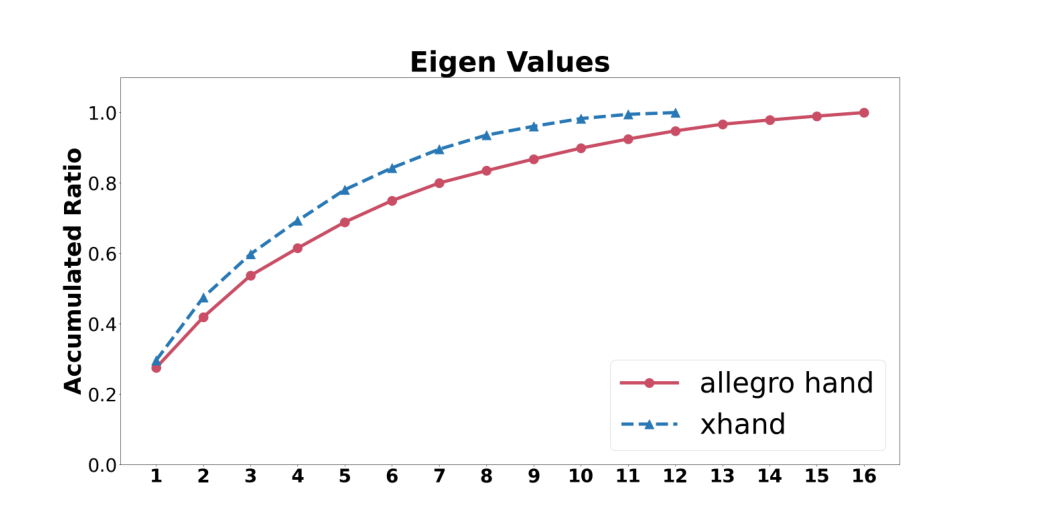
\includegraphics[width=0.5\linewidth,keepaspectratio]{figs/dex_eigengrasp.png}
   \caption{Accumulated variance ratio versus eigengrasp dimension for the Allegro Hand and the XHand \cite{p1}}
   \label{fig:dex_eigen}
\end{figure}

\paragraph{} \textbf{Dense reward design.} To guide the search efficiently, dense rewards are defined for each end effector. Common to all are a success reward and an approaching reward:
\begin{equation}
r_{\mathrm{success}}=\begin{cases}\omega_s, & |s_{\mathrm{target}}-s_t|<\epsilon\\ 0, & \text{otherwise}\end{cases},\qquad
r_{\mathrm{target}}=-\omega_t\,\frac{|s_{\mathrm{target}}-s_t|}{|s_{\mathrm{target}}-s_{\mathrm{initial}}|}.
\end{equation}
A contact reward encourages correct, sustained contact and penalizes collisions:
\begin{equation}
r_{\mathrm{contact}}=\begin{cases}\omega_{\mathrm{contact}}, & \dfrac{|s_t-s_{\mathrm{target}}|}{|s_{\mathrm{target}}-s_{\mathrm{initial}}|}<1\\[4pt] -\omega_{\mathrm{collision}}, & \text{unexpected collision}\\ 0, & \text{otherwise.}\end{cases}
\end{equation}
A distance term $r_{\mathrm{dist}}$, weighted by $\omega_d$ and computed from $\|p_{\mathrm{part}}-p_{\mathrm{grasp}}\|_2^2$, draws the end effector (or, for suction, a virtual link at the suction tip) towards the geometric centre of the target part. The suction gripper additionally receives an access-direction reward $r_{\mathrm{dir}}=\omega_{\mathrm{dir}}$ when the angle between the suction axis and the target surface normal is within a threshold $\psi$. The two-finger gripper uses a regularization reward $r_{\mathrm{reg}}=-\sum_{i=1}^{d}(\omega_a a_i+\omega_v v_i)$ that penalizes joint accelerations and velocities. For the dexterous hand, the contact reward is granted only when the palm \emph{and} at least two fingers touch the object, encouraging the hand to cage the part, and the regularization $r_{\mathrm{reg}}=-\omega_p e_p-\sum_i \omega_v v_i$ also penalizes the Cartesian error $e_p$ of the end link.

\subsection{Experimental Setup}

\paragraph{} Real-world experiments use a 7-DOF ROKAE xMate3Pro arm fixed to a table, an Intel RealSense D415 RGB-D camera (the only sensor that requires calibration), and an additional side RGB camera. Four end effectors are evaluated: a suction gripper, a Robotiq 2F-140 two-finger gripper, a 16-DOF four-finger Allegro Hand, and a 12-DOF five-finger XHand. Test objects come from four categories---drawers, cabinets, lamps, and laptops---placed at random positions with random initial and goal joint states covering both directions of motion. Joint states after manipulation are measured with a double-arm protractor. SAPIEN is used both to train the affordance network and as the MPC simulator. The planner runs 30 sampling processes on a workstation with an AMD Ryzen 9 9950X CPU and an NVIDIA RTX 3080Ti GPU. Table~\ref{tab:dex_params} lists the planning parameters.

{\renewcommand{\arraystretch}{1.2}
\begin{table}[htbp]
\centering
\caption{Sampling-based MPC settings used in DexSim2Real$^2$ \cite{p1}}\label{tab:dex_params}
\small
\begin{tabular}{|l|c|c|c|c|c|}
\hline
\textbf{End effector} & \textbf{Action dim.} $d$ & $T$ & $E$ & $h$ & \textbf{Search time} \\ \hline
Suction gripper & 7 & 50 & 20 & 10 & $\approx$1.5 min \\ \hline
Two-finger gripper (Robotiq 2F-140) & 8 & 50 & 300 & 10 & $\approx$2.5 min \\ \hline
Dexterous hand (Allegro, $m=2$) & $7+m=9$ & 50 & 100 & 10 & $\approx$3 min \\ \hline
\end{tabular}
\end{table}}

\paragraph{} Joint increments are limited to $[-0.05,0.05]$ per step. For the suction gripper the reward weights are $\omega_s=20$, $\omega_t=50$, $\omega_{\mathrm{contact}}=10$, $\omega_{\mathrm{collision}}=60$, $\omega_d=10$, $\omega_a=0.01$, $\omega_v=0.03$, $\psi=15^{\circ}$, with success thresholds $\epsilon=0.005$ for prismatic and $0.02$ for revolute joints. For VRB-based affordance, the virtual camera is placed at $(0.2,0,0.7)$ in the robot base frame with a pitch of $52^{\circ}$, balancing visual similarity against the baseline required for accurate plane intersection.

\subsection{Results and Analysis}

\paragraph{} \textbf{Suction gripper versus UMPNet.} UMPNet, which also performs goal-conditioned articulated manipulation, is used as the baseline on laptops and cabinets with ten trials each. Table~\ref{tab:dex_suction} and Figure~\ref{fig:dex_charts}(a) show that DexSim2Real$^2$ roughly halves the error: $7.2^{\circ}$ versus $16.0^{\circ}$ on laptops and $6.8^{\circ}$ versus $15.3^{\circ}$ on cabinets. The authors attribute UMPNet's larger error to its fixed step size and to the limited information in a pair of current/goal images, whereas MPC over an explicit model uses continuous actions.

{\renewcommand{\arraystretch}{1.2}
\begin{table}[htbp]
\centering
\caption{Accuracy of real articulated object manipulation with the suction gripper \cite{p1}}\label{tab:dex_suction}
\small
\begin{tabular}{|l|c|c|c|c|}
\hline
\multirow{2}{*}{\textbf{Metric}} & \multicolumn{2}{c|}{\textbf{Laptop}} & \multicolumn{2}{c|}{\textbf{Cabinet}} \\ \cline{2-5}
 & UMPNet & Ours & UMPNet & Ours \\ \hline
Trials with $|\delta_r|<10\%$ ($\uparrow$) & 0/10 & \textbf{3/10} & 0/10 & \textbf{4/10} \\ \hline
Trials with $|\delta_r|<30\%$ ($\uparrow$) & 3/10 & \textbf{9/10} & 5/10 & \textbf{7/10} \\ \hline
Trials with $|\delta_r|<50\%$ ($\uparrow$) & 7/10 & \textbf{9/10} & 6/10 & \textbf{8/10} \\ \hline
Average $|\delta|$ ($\downarrow$) & $16.0^{\circ}$ & $\mathbf{7.2^{\circ}}$ & $15.3^{\circ}$ & $\mathbf{6.8^{\circ}}$ \\ \hline
Average $|\delta_r|$ ($\downarrow$) & 42.9\% & \textbf{23.3\%} & 41.5\% & \textbf{21.7\%} \\ \hline
\end{tabular}
\end{table}}

\paragraph{} \textbf{Two-finger gripper.} Twenty trials each on laptops and cabinets (Table~\ref{tab:dex_2f}) yield average errors of $7.2^{\circ}$ and $7.4^{\circ}$, with about 75\% of manipulations achieving $|\delta_r|<30\%$. A reward ablation on four tasks (opening/closing a drawer and a laptop) shows that the full reward achieves the best success rate and fewest steps, except when $r_{\mathrm{reg}}$ is removed; however, trajectories found without $r_{\mathrm{reg}}$ drive the robot into unusual and potentially dangerous configurations. Without $r_{\mathrm{dist}}$ the task cannot be completed at all, because the short planning horizon never reaches positive reward, and removing $r_{\mathrm{target}}$, $r_{\mathrm{success}}$, or $r_{\mathrm{contact}}$ lowers success and lengthens trajectories.

\paragraph{} \textbf{Dexterous hand.} Using the Allegro Hand with $m=2$, twenty trials each on drawers and cabinets give an average error of 1.64 cm for prismatic drawers and $6.87^{\circ}$ for revolute cabinets (Table~\ref{tab:dex_2f}). All forty manipulations achieve $|\delta_r|<50\%$.

{\renewcommand{\arraystretch}{1.2}
\begin{table}[htbp]
\centering
\caption{Accuracy of real manipulation with the two-finger gripper and the dexterous hand \cite{p1}}\label{tab:dex_2f}
\small
\begin{tabular}{|l|c|c|c|c|}
\hline
\multirow{2}{*}{\textbf{Metric}} & \multicolumn{2}{c|}{\textbf{Two-finger gripper}} & \multicolumn{2}{c|}{\textbf{Dexterous hand}} \\ \cline{2-5}
 & Laptop & Cabinet & Drawer & Cabinet \\ \hline
Number of manipulations & 20 & 20 & 20 & 20 \\ \hline
$|\delta_r|<10\%$ & 6 & 4 & 3 & 3 \\ \hline
$|\delta_r|<30\%$ & 16 & 15 & 11 & 18 \\ \hline
$|\delta_r|<50\%$ & 20 & 18 & 20 & 20 \\ \hline
Average $|\delta|$ & $7.2^{\circ}$ & $7.4^{\circ}$ & 1.64 cm & $6.87^{\circ}$ \\ \hline
Average $|\delta_r|$ & 21.5\% & 22.5\% & 26.4\% & 20.4\% \\ \hline
\end{tabular}
\end{table}}

\paragraph{} \textbf{Effect of eigengrasp dimension.} Simulation experiments with $m\in\{1,2,7,16\}$ on four tasks (ten randomized repetitions each) evaluate success rate, joint jerk, and computation time. Opening a laptop and closing a drawer succeed 100\% of the time for all $m$, but closing a laptop and opening a drawer fail more often with $m=1$ because the hand loses dexterity. Crucially, $m=2$ performs comparably to $m=7$ and $m=16$, while finger jerk grows with $m$ and $m=2$ saves roughly one second per planning step compared with $m=16$---nearly one minute per trajectory. A dexterous-hand reward ablation shows the same pattern as for the gripper, with the interesting exception that removing $r_{\mathrm{contact}}$ sometimes shortens trajectories, because the planner is then free to explore unconventional, non-human-like hand postures.

\paragraph{} \textbf{Dexterous hand versus two-finger gripper.} On five simulated tasks with ten randomized initial conditions each, the Allegro Hand requires fewer steps than the Robotiq gripper on every task except laptop opening, which does not require precise contact. For example, the dexterous hand opens a drawer in 17 steps versus 22 for the gripper by exploiting its additional degrees of freedom.

\paragraph{} \textbf{World model construction accuracy.} The digital twins are evaluated with the Relative Depth Error (RDE) between rendered and real depth, the IoU between rendered and ground-truth masks, and the joint axis position and angle errors. Table~\ref{tab:dex_model} and Figure~\ref{fig:dex_charts}(b) compare the axis angle error with ScrewNet. The average angle error is below $9^{\circ}$ for all four categories, far lower than ScrewNet on laptops ($1.34^{\circ}$ vs.\ $23.15^{\circ}$) and drawers ($8.58^{\circ}$ vs.\ $23.21^{\circ}$). The lower IoU for lamps is attributed to their small image footprint. Deliberately corrupting the model shows that manipulation error correlates positively with modelling error, with joint \emph{position} errors having a stronger effect than orientation errors.

{\renewcommand{\arraystretch}{1.2}
\begin{table}[htbp]
\centering
\caption{Explicit world model construction accuracy \cite{p1}}\label{tab:dex_model}
\small
\begin{tabular}{|l|c|c|c|c|c|}
\hline
\textbf{Category} & \textbf{RDE (\%)} & \textbf{IoU} & \shortstack{\textbf{Pos.}\\\textbf{err. (m)}} & \shortstack{\textbf{Angle}\\\textbf{err. ($^{\circ}$)}} & \shortstack{\textbf{ScrewNet angle}\\\textbf{err. ($^{\circ}$)}} \\ \hline
Laptop & 1.47 & 0.92 & 0.022 & 1.34 & 23.15 \\ \hline
Cabinet & 3.77 & 0.94 & 0.029 & 4.84 & 11.67 \\ \hline
Drawer & 2.23 & 0.94 & -- & 8.58 & 23.21 \\ \hline
Lamp & 2.12 & 0.80 & 0.009 & 7.95 & 9.38 \\ \hline
\end{tabular}
\end{table}}

\begin{figure}[htbp]
\centering
\begin{subfigure}[b]{0.47\textwidth}
\centering
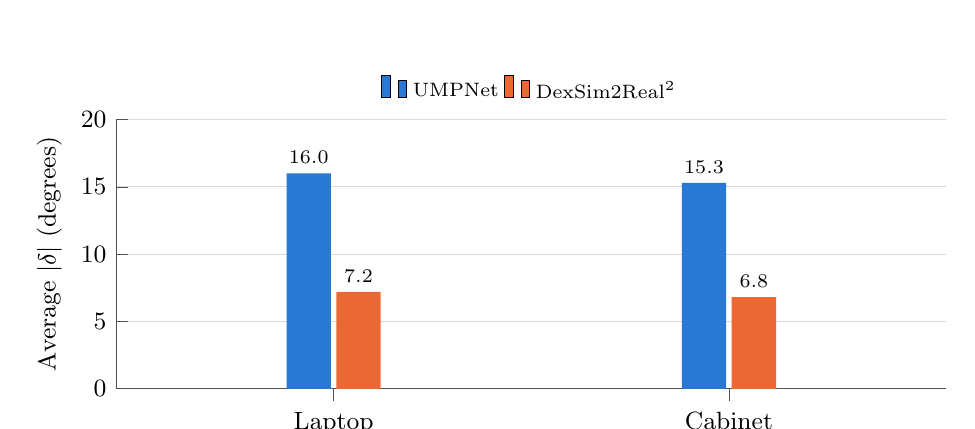
\begin{tikzpicture}
\begin{axis}[
  ybar=2pt, bar width=16pt, width=\linewidth, height=5cm,
  symbolic x coords={Laptop,Cabinet}, xtick=data, enlarge x limits=0.55,
  ymin=0, ymax=20, ylabel={Average $|\delta|$ (degrees)}, ylabel style={font=\small},
  ymajorgrids, grid style={gridgray}, axis line style={inkgray}, tick style={inkgray},
  axis x line*=bottom, axis y line*=left, tick label style={font=\small},
  nodes near coords, nodes near coords style={font=\scriptsize, text=black},
  every node near coord/.append style={/pgf/number format/fixed, /pgf/number format/fixed zerofill, /pgf/number format/precision=1},
  legend style={at={(0.5,1.02)}, anchor=south, legend columns=-1, draw=none, font=\scriptsize},
]
\addplot[fill=seriesA, draw=none] coordinates {(Laptop,16.0) (Cabinet,15.3)};
\addplot[fill=seriesB, draw=none] coordinates {(Laptop,7.2) (Cabinet,6.8)};
\legend{UMPNet, DexSim2Real$^2$}
\end{axis}
\end{tikzpicture}
\caption{Suction-gripper manipulation error}
\end{subfigure}\hfill
\begin{subfigure}[b]{0.5\textwidth}
\centering
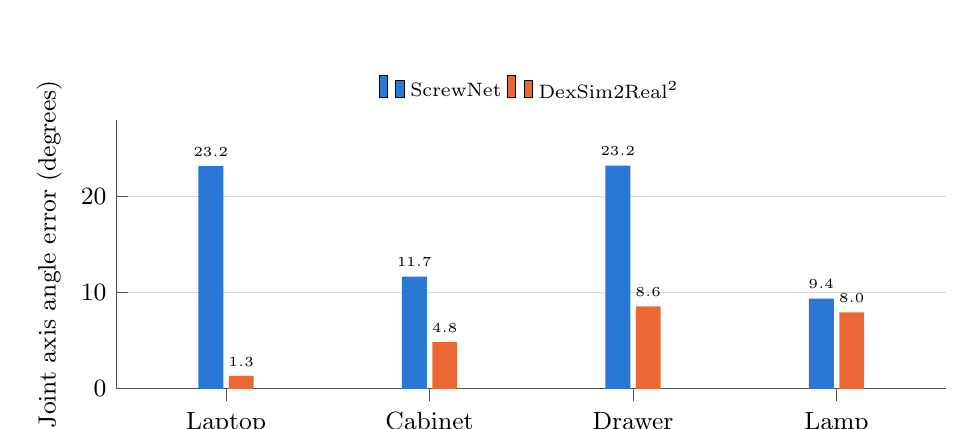
\begin{tikzpicture}
\begin{axis}[
  ybar=2pt, bar width=9pt, width=\linewidth, height=5cm,
  symbolic x coords={Laptop,Cabinet,Drawer,Lamp}, xtick=data, enlarge x limits=0.18,
  ymin=0, ymax=28, ylabel={Joint axis angle error (degrees)}, ylabel style={font=\small},
  ymajorgrids, grid style={gridgray}, axis line style={inkgray}, tick style={inkgray},
  axis x line*=bottom, axis y line*=left, tick label style={font=\small},
  nodes near coords, nodes near coords style={font=\tiny, text=black},
  every node near coord/.append style={/pgf/number format/fixed, /pgf/number format/fixed zerofill, /pgf/number format/precision=1},
  legend style={at={(0.5,1.02)}, anchor=south, legend columns=-1, draw=none, font=\scriptsize},
]
\addplot[fill=seriesA, draw=none] coordinates {(Laptop,23.15) (Cabinet,11.67) (Drawer,23.21) (Lamp,9.38)};
\addplot[fill=seriesB, draw=none] coordinates {(Laptop,1.34) (Cabinet,4.84) (Drawer,8.58) (Lamp,7.95)};
\legend{ScrewNet, DexSim2Real$^2$}
\end{axis}
\end{tikzpicture}
\caption{Model construction: joint axis angle error}
\end{subfigure}
\caption{Quantitative results of DexSim2Real$^2$ plotted from the values reported in \cite{p1} (lower is better)}
\label{fig:dex_charts}
\end{figure}

\paragraph{} \textbf{Ablation of movable part segmentation and affordance.} Without the proposed segmentation module (i.e.\ jointly optimizing segmentation and motion as in the method of Liu et al.), model construction succeeds on only 5/10 drawers instead of 10/10 and the drawer axis error doubles from $8.58^{\circ}$ to $16.04^{\circ}$; position errors also increase for laptops (0.022 to 0.048 m), cabinets, and lamps, and the baseline sometimes produces the wrong number of parts or wrong joint types. For affordance detection on closed objects, VRB finds handles on 17/20 cabinets versus 7/20 for Where2Act, and on 3/20 versus 1/20 small drawer handles; in over 90\% of real-world cases VRB proposes the better action, which the authors attribute to its training on real human videos and to the larger scale of video data compared with interactable 3D assets. The pixel projection method also produces better interaction directions than random 3D vectors consistent with the 2D affordance.

\paragraph{} \textbf{Multi-part objects and tool use.} Figure~\ref{fig:dex_multi}(a) shows reconstructed twins of a cabinet with two revolute doors and a refrigerator with two revolute joints and one prismatic joint, demonstrating that the pipeline handles varied kinematic structures. Because the world model is a physics simulator, it generalizes to actions never observed during interaction: when a drawer is out of reach or its gap is too small for the gripper, the robot can use a T-shaped tool or a semi-ring (Figure~\ref{fig:dex_multi}(b)). The only change needed is to replace the gripper tips with the tool in $r_{\mathrm{dist}}$; most other parameters are unchanged.

\begin{figure}[htbp]
\centering
\begin{subfigure}[b]{0.36\textwidth}
  \centering
  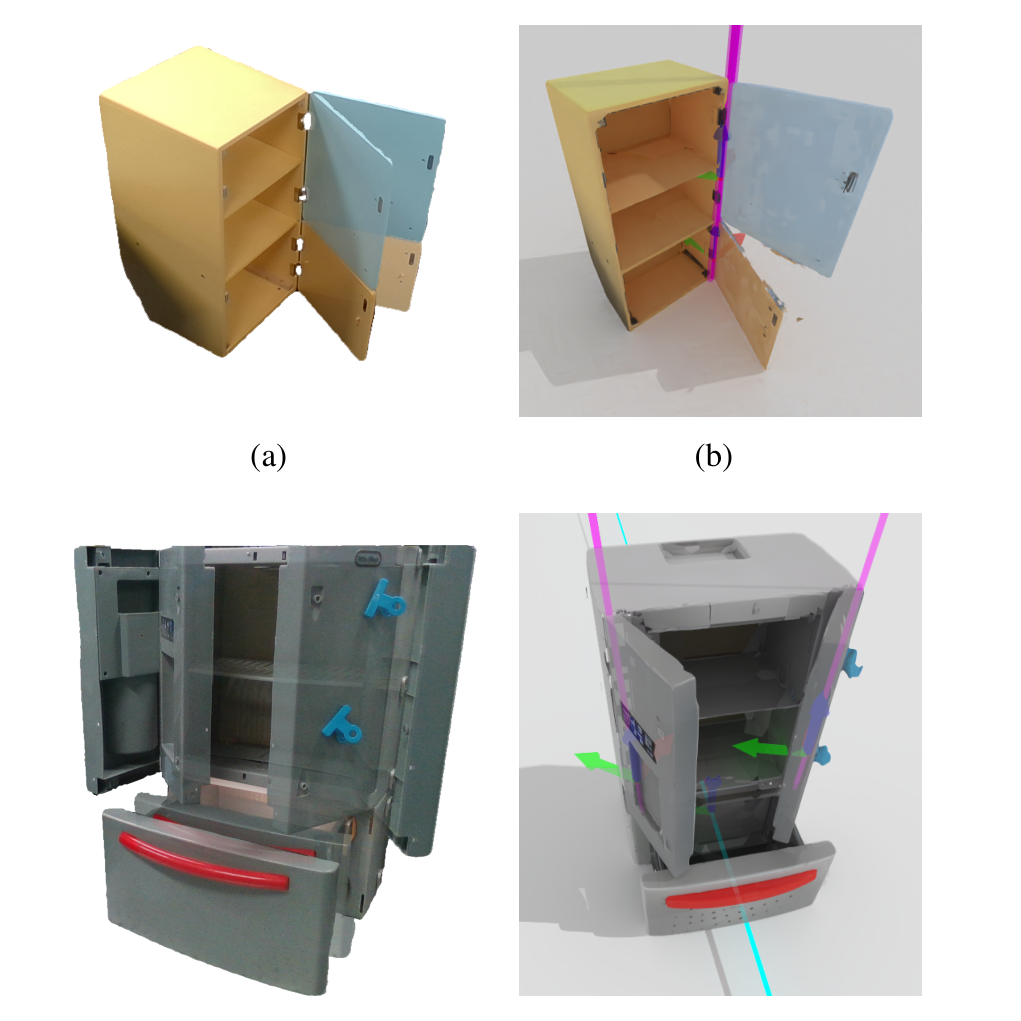
\includegraphics[width=\linewidth,keepaspectratio]{figs/dex_multipart.png}
  \caption{Multi-part objects and their twins}
\end{subfigure}\hfill
\begin{subfigure}[b]{0.6\textwidth}
  \centering
  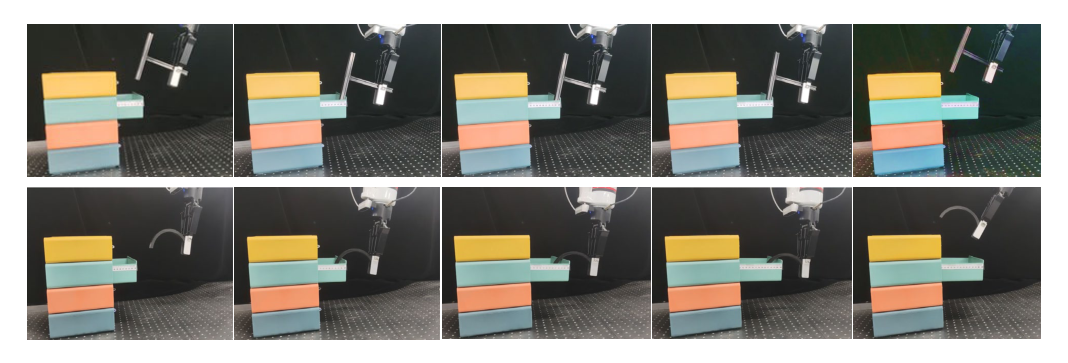
\includegraphics[width=\linewidth,keepaspectratio]{figs/dex_tools.png}
  \caption{Opening a small drawer with a T-shaped tool (top) and a semi-ring (bottom)}
\end{subfigure}
\caption{Generalization of the explicit world model: (a) reconstructed twins of a cabinet with two revolute joints and a refrigerator with two revolute joints (pink) and one prismatic joint (blue); (b) tool use planned entirely in the world model \cite{p1}}
\label{fig:dex_multi}
\end{figure}

\subsection{Discussion}

\paragraph{}
By first building the world model of a single object instance and then planning within it, the framework avoids the data-hungry generalization burden of policy networks. The explicit physics prior guarantees that a model constructed from simple one-step interactions supports long-horizon, multi-step, and even unseen tool-using trajectories, marking a distinctive advantage over articulation-flow and policy-based baselines. The authors identify two sources of residual error beyond modelling inaccuracy: real objects have complex dynamics (a laptop lid deforms elastically and partially springs back when released), and real joints are not ideal (rail gaps turn a prismatic joint into a joint with several degrees of freedom). The method also requires every movable part to change observably during interactive perception, and 3D AIGC may produce misaligned meshes for novel or uncommon objects. The authors propose extending the framework to scene-level digital twins for long-horizon mobile manipulation and generating rewards from videos.

%---------------------------------------------------------------

\section{GAF: Gaussian Action Field as a 4D Representation for Dynamic World Modeling in Robotic Manipulation}

This research introduces a Vision-to-4D-to-Action (V-4D-A) paradigm in which manipulation actions are reasoned directly from a motion-aware 4D scene representation \cite{p2}. The Gaussian Action Field (GAF) extends 3D Gaussian Splatting (3DGS) with a learnable motion attribute per Gaussian, so that a single feed-forward network simultaneously reconstructs the current scene, predicts the future scene, and yields an initial estimate of the robot action from the predicted Gaussian motion.

\subsection{Problem Statement and Motivation}

\paragraph{} Vision-based manipulation methods fall into two paradigms (Figure~\ref{fig:gaf_paradigm}). \textbf{V-A} (vision-to-action) methods such as Diffusion Policy map images directly to actions; they benefit from end-to-end learning and large image datasets but understand 3D structure only implicitly and struggle in high-precision tasks. \textbf{V-3D-A} (vision-to-3D-to-action) methods such as Act3D lift observations to point clouds or voxels, capturing spatial relationships more accurately, but require 3D data that is scarcer than images. Both share a deeper limitation: they model a \emph{static} snapshot of the scene, even though manipulation is inherently about how the scene---including the robot itself---will change. This creates a mismatch between static scene understanding and dynamic action generation. Prior Gaussian world models such as ManiGaussian and GWM deform Gaussians to predict the future, but use the prediction only as auxiliary supervision for policy training, and their low-fidelity reconstructions limit effectiveness.

\begin{figure}[htbp]
   \centering
   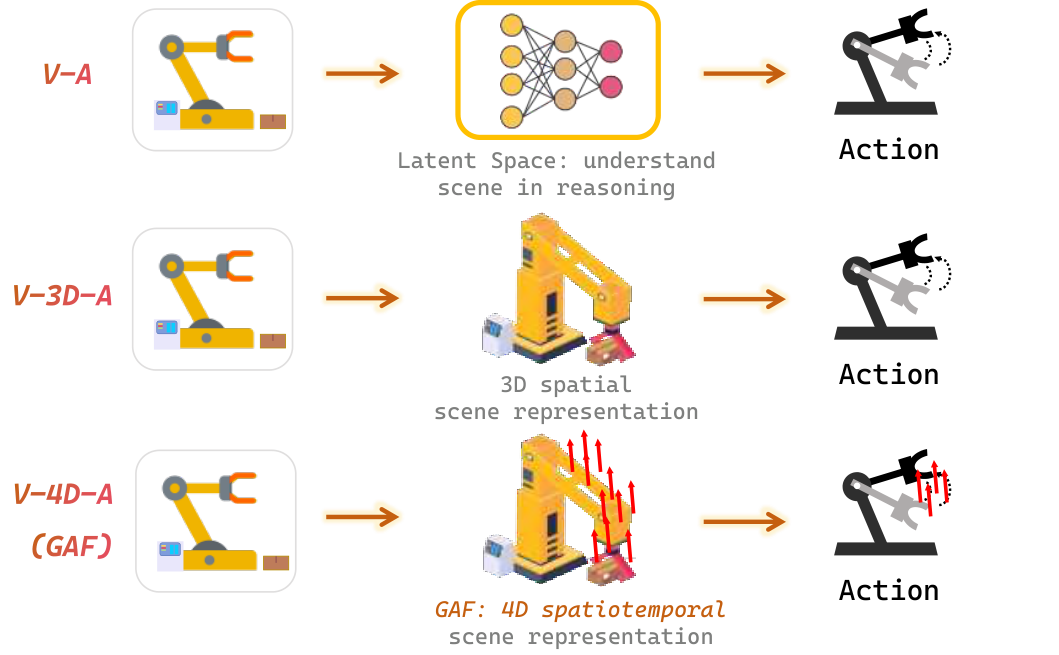
\includegraphics[width=0.5\linewidth,keepaspectratio]{figs/gaf_paradigms.png}
   \caption{Comparison of the V-A, V-3D-A, and the proposed V-4D-A (GAF) paradigms \cite{p2}}
   \label{fig:gaf_paradigm}
\end{figure}

\subsection{The Gaussian Action Field Representation}

\paragraph{} GAF is defined as a unified spatiotemporal representation that associates each Gaussian primitive $g(x)$ at time $t$ with both geometric attributes and motion dynamics, parameterized by a continuous function
\begin{equation}
\mathcal{F}_\Theta:\;\{g(x),t\}\mapsto\{\mu,\;\Delta\mu,\;f\},
\end{equation}
where $\mu\in\mathbb{R}^3$ is the Gaussian's position, $\Delta\mu\in\mathbb{R}^3$ its displacement over a future interval, and $f=\{c,\sigma,r,s\}$ its colour, opacity, rotation, and scale. Three outputs are derived: the \textbf{current Gaussians} $\{\mu,f\}$ representing the present scene; the \textbf{future Gaussians} $\{\mu+\Delta\mu,f\}$ representing how the scene will evolve; and the \textbf{init action}, obtained by registering the current and future Gaussians that belong to the manipulator.

\subsection{Architecture: Dynamic Gaussian Reconstruction}

\paragraph{} GAF adopts a geometry-agnostic, \emph{pose-free} reconstruction approach. Unlike NeRF or classical 3DGS, which require dense calibrated views or geometric priors such as cost volumes, GAF reconstructs motion-augmented Gaussians from only two unposed RGB images and their intrinsics $\{I^t_v,k^t_v\}_{v=1}^{V}$, in a canonical frame aligned with the first view (Figure~\ref{fig:gaf_recon}). The images are split into patches, concatenated, and processed by a shared-weight Vision Transformer with cross-view attention, initialized from MASt3R. Three DPT-style heads decode the features: a Gaussian Center Head $h_{\mathrm{center}}$ predicts positions, a Gaussian Params Head $h_{\mathrm{feature}}$ predicts appearance, and a Motion Prediction Head $h_{\mathrm{motion}}$ predicts per-point displacements:
\begin{align}
\mathcal{H}_{\mathrm{Gauss}}\big(\mathrm{ViT}(\{I^t_v,k^t_v\}_{v=1}^{V})\big) &= \{\mu^t_j,c^t_j,\sigma^t_j,r^t_j,s^t_j\}_{j=1}^{V\times H\times W},\\
h_{\mathrm{motion}}\big(\mathrm{ViT}(\{I^t_v,k^t_v\}_{v=1}^{V})\big) &= \{\Delta\mu^{t\to t+\Delta t}_j\}.
\end{align}

\begin{figure}[htbp]
   \centering
   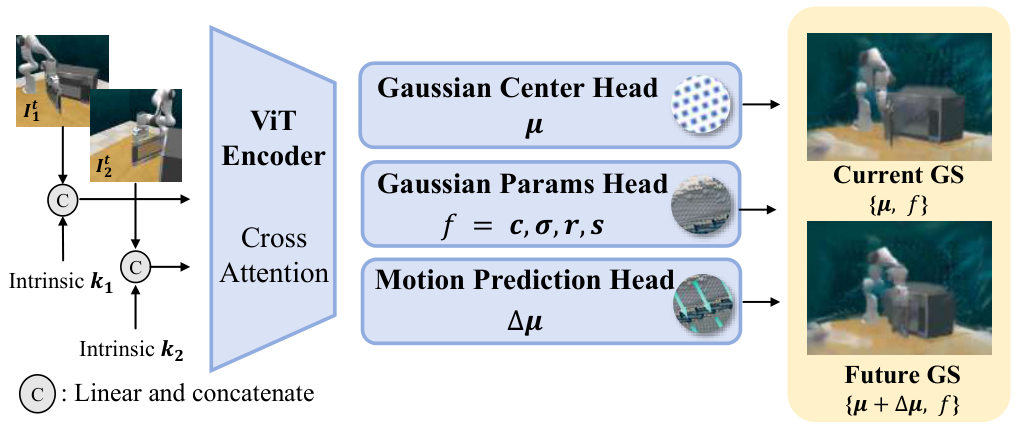
\includegraphics[width=0.6\linewidth,keepaspectratio]{gaf_reconstruction.png}
   \caption{GAF reconstruction: a ViT with cross-view attention and three heads predicts Gaussian centres, appearance parameters, and motion \cite{p2}}
   \label{fig:gaf_recon}
\end{figure}

\paragraph{} Adding the displacements to the centres gives the future Gaussians. Both current and future Gaussians are rendered to $M$ novel views using the alpha-blending rule of Equation~(\ref{eq:alphablend}), which allows the whole network to be trained purely from RGB video frames, without depth, camera poses, 3D ground truth, or action labels. The training objective combines perceptual and pixel losses on both time steps:
\begin{equation}
\mathcal{L}_{\mathrm{GAF}}=\mathcal{L}^{t}_{\mathrm{LPIPS}}+\mathcal{L}^{t}_{\mathrm{MSE}}+\mathcal{L}^{t+\Delta t}_{\mathrm{LPIPS}}+\mathcal{L}^{t+\Delta t}_{\mathrm{MSE}},
\end{equation}
where the $t$ terms enforce fidelity to the current observation and the $t+\Delta t$ terms regularize future prediction.

\subsection{Init Action Computation}

\paragraph{} Because the gripper is rigid, its motion between the current and predicted future scenes is a rigid transformation. GAF extracts the gripper Gaussians $\mu_{\mathrm{gripper}}$ and their future counterparts $(\mu+\Delta\mu)_{\mathrm{gripper}}$ and estimates the end-effector transformation $T^{t\to t+\Delta t}\in SE(3)$ with Iterative Closest Point (ICP):
\begin{equation}
T^{t\to t+\Delta t}=\arg\min_{T}\sum_{k\in\mathrm{gripper}}\big\|T(\mu_k)-(\mu+\Delta\mu)_k\big\|^2 .
\end{equation}
This transformation is interpolated into a sequence over discrete time steps, forming the init action $a_{\mathrm{init}}$. In this way, the action is not predicted by a separate policy head but \emph{read out} of the predicted future geometry.

\subsection{Manipulation with GAF: Action-Vision-Aligned Denoising}

\paragraph{} Since GAF is trained only on visual data, its init actions are visually plausible but not necessarily physically feasible. A refinement stage (Figure~\ref{fig:paper2_wm}) therefore uses a diffusion model and a small amount of real action data, following Render-and-Diffuse. For a candidate relative action $a$, the gripper's new world pose is $T^{w}_{g_{\mathrm{new}}}=T^{w}_{g}\times a$, and its CAD model is rendered into each calibrated camera $c$:
\begin{equation}
R_c=\mathrm{Render}\big(T_{w2c}\times T^{w}_{g}\times a,\;K_c\big).
\end{equation}
Overlaying these renderings on the current multi-view images produces the \textbf{Actionable Multiview RGB Guidance}, which places the visual observation and the candidate action in a single image space. The diffusion model is trained with
\begin{equation}
\mathcal{L}_{\mathrm{refine}}=L_1(D,D_{gt})+L_1(\epsilon,\epsilon_{gt})+\mathrm{BCE}(g,g_{gt}),
\end{equation}
where $D$ is the denoising direction of the gripper, $\epsilon$ the noise added to the end-effector action, and $g$ the binary gripper open/close state. The denoised poses are executed with inverse kinematics, new observations are collected, and the loop repeats until the task is complete, providing closed-loop robustness to occlusion and interaction uncertainty.

\begin{figure}[htbp]
   \centering
   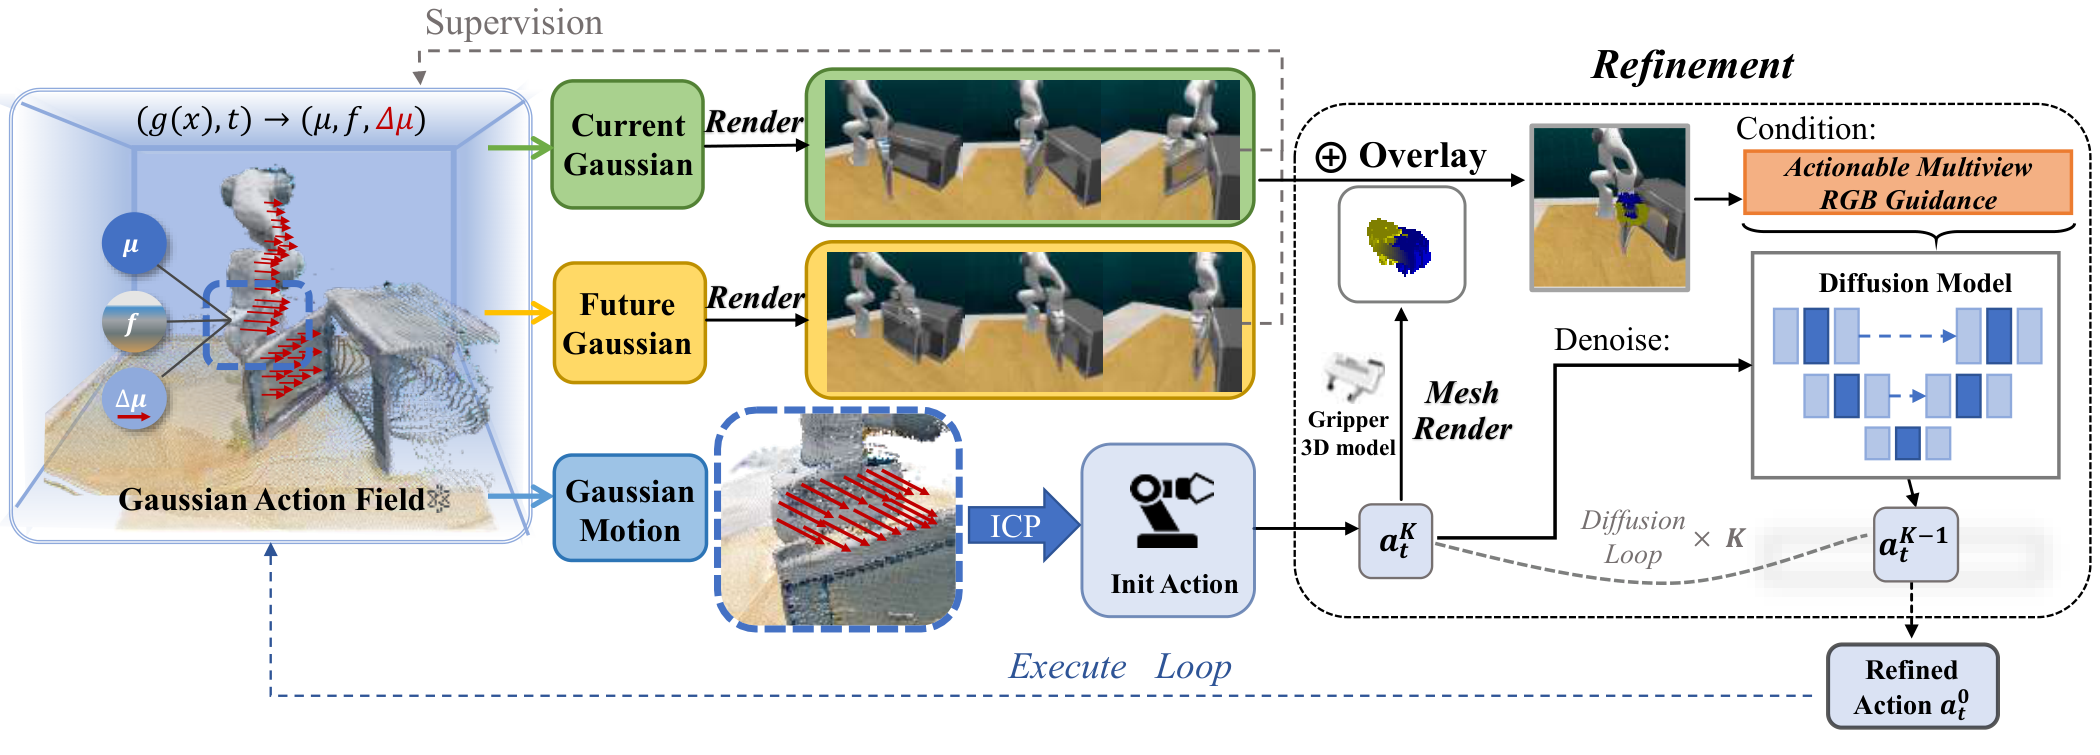
\includegraphics[width=0.92\linewidth,height=.26\textheight,keepaspectratio]{gaf_pipeline.png}
   \caption{GAF manipulation pipeline with action-vision-aligned denoising \cite{p2}}
   \label{fig:paper2_wm}
\end{figure}

\subsection{Experimental Setup and Implementation}

\paragraph{} Simulation experiments use nine RLBench tasks covering fine-grained placement, occlusion-rich interactions, and articulated objects, with 20 demonstrations per task and evaluation on 100 unseen object poses. Baselines are Diffusion Policy (V-A), Act3D (V-3D-A), and ManiGaussian (Gaussian world model), with hyper-parameters matched for fairness. All methods use two external cameras and a wrist camera ($128\times128$ in simulation, $1280\times720$ in the real world). Table~\ref{tab:gaf_impl} summarizes implementation details.

{\renewcommand{\arraystretch}{1.2}
\begin{table}[htbp]
\centering
\caption{Implementation details of GAF \cite{p2}}\label{tab:gaf_impl}
\small
\begin{tabularx}{\textwidth}{|p{4.3cm}|X|}
\hline
\textbf{Item} & \textbf{Setting} \\ \hline
Reconstruction backbone & ViT with cross-view attention, initialized from MASt3R; DPT heads \\ \hline
GAF training & 80k iterations, batch size 16, single NVIDIA A800 GPU, about 24 hours \\ \hline
Diffusion training & 50 DDIM iterations; 1 past observation in, 8 future actions out; 50k iterations in about 1.5 days on a single GPU \\ \hline
Inference & 3 diffusion iterations; each 8-step action prediction takes less than 0.3 s \\ \hline
Real-world deployment & Prediction and execution run in parallel threads to hide latency \\ \hline
\end{tabularx}
\end{table}}

\subsection{Results and Analysis}

\paragraph{} \textbf{Manipulation success on RLBench.} Table~\ref{tab:gaf_rlbench} and Figure~\ref{fig:gaf_chart} show that GAF achieves the highest average success rate of 60.4\%, improving on Diffusion Policy by 15.7 points, on Act3D by 7.3 points, and on ManiGaussian by 10.3 points. Gains are largest on occlusion-heavy tasks such as \emph{Toilet Seat Down} (71\% versus 39\% for DP), highlighting the value of 3D and 4D perception. Removing GAF (predicting actions from images with a diffusion model starting from random noise, without multi-view rendering or init-action priors) reduces the average by 9.1 points to 51.3\%.

{\renewcommand{\arraystretch}{1.25}
\begin{table}[htbp]
\centering
\caption{Success rates (\%) on nine RLBench tasks \cite{p2}}\label{tab:gaf_rlbench}
\footnotesize
\setlength{\tabcolsep}{4pt}
\begin{tabular}{|l|c|c|c|c|c|c|c|c|c|c|}
\hline
\textbf{Method} & \rotatebox{90}{\textbf{Toilet seat down}} & \rotatebox{90}{\textbf{Open grill}} & \rotatebox{90}{\textbf{Close grill}} & \rotatebox{90}{\textbf{Close fridge}} & \rotatebox{90}{\textbf{Phone on base}} & \rotatebox{90}{\textbf{Lift lid up}} & \rotatebox{90}{\textbf{Close microwave}} & \rotatebox{90}{\textbf{Push button}} & \rotatebox{90}{\textbf{Close laptop}} & \rotatebox{90}{\textbf{Average}} \\ \hline
Diffusion Policy & 39 & 20 & 36 & 16 & 23 & 81 & 62 & 61 & 64 & 44.7 \\ \hline
Act3D & 60 & 22 & 41 & \textbf{47} & 26 & 91 & 73 & 60 & 58 & 53.1 \\ \hline
ManiGaussian & 34 & 24 & 38 & 41 & 30 & 97 & 67 & \textbf{63} & 57 & 50.1 \\ \hline
Ours w/o GAF & 57 & 16 & 49 & 27 & 31 & 94 & 79 & 58 & 51 & 51.3 \\ \hline
\textbf{GAF (ours)} & \textbf{71} & \textbf{26} & \textbf{55} & 42 & \textbf{35} & \textbf{100} & \textbf{85} & 61 & \textbf{69} & \textbf{60.4} \\ \hline
\end{tabular}
\end{table}}

\begin{figure}[htbp]
\centering
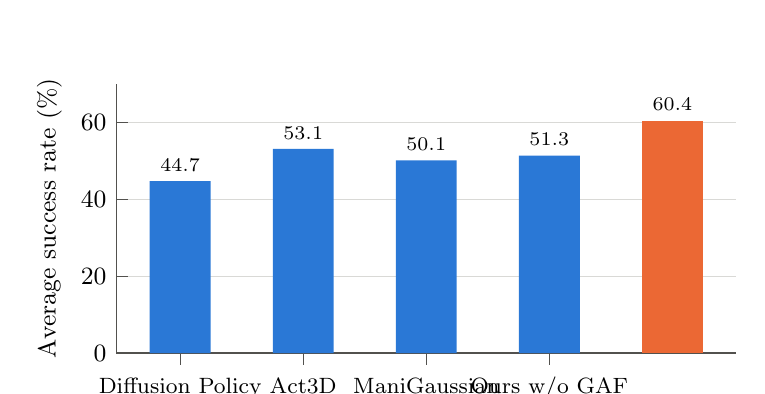
\begin{tikzpicture}
\begin{axis}[
  ybar, bar width=22pt, width=0.78\textwidth, height=5cm,
  symbolic x coords={Diffusion Policy,Act3D,ManiGaussian,Ours w/o GAF,GAF},
  xtick=data, enlarge x limits=0.13, ymin=0, ymax=70,
  ylabel={Average success rate (\%)}, ylabel style={font=\small},
  ymajorgrids, grid style={gridgray}, axis line style={inkgray}, tick style={inkgray},
  axis x line*=bottom, axis y line*=left, tick label style={font=\small},
  x tick label style={font=\footnotesize},
  nodes near coords, nodes near coords style={font=\scriptsize, text=black},
  every node near coord/.append style={/pgf/number format/fixed, /pgf/number format/fixed zerofill, /pgf/number format/precision=1},
]
\addplot[fill=seriesA, draw=none, bar shift=0pt] coordinates {(Diffusion Policy,44.7) (Act3D,53.1) (ManiGaussian,50.1) (Ours w/o GAF,51.3)};
\addplot[fill=seriesB, draw=none, bar shift=0pt] coordinates {(GAF,60.4)};
\end{axis}
\end{tikzpicture}
\caption{Average RLBench success rate of GAF (orange) compared with baselines and its own ablation (blue), plotted from \cite{p2}}
\label{fig:gaf_chart}
\end{figure}

\paragraph{} \textbf{Scene reconstruction and prediction.} Compared with ManiGaussian on three tasks, GAF improves current-scene reconstruction by +11.54 dB PSNR, +0.386 SSIM, and $-0.557$ LPIPS on average, and future-scene prediction by +10.53 dB PSNR, +0.386 SSIM, and $-0.576$ LPIPS (Table~\ref{tab:gaf_nvs}). Qualitatively, GAF preserves fine structures such as the gripper's articulated joints even under partial observation, which is exactly what makes ICP-based action extraction possible. Dynamic reconstruction methods such as 4DGS are not compared because they interpolate between observed frames rather than predicting future states.

{\renewcommand{\arraystretch}{1.2}
\begin{table}[htbp]
\centering
\caption{Average novel-view synthesis quality for current and future scenes (three RLBench tasks) \cite{p2}}\label{tab:gaf_nvs}
\small
\begin{tabular}{|l|c|c|c|}
\hline
\textbf{Method / state} & \textbf{PSNR} $\uparrow$ & \textbf{SSIM} $\uparrow$ & \textbf{LPIPS} $\downarrow$ \\ \hline
ManiGaussian / current & 16.38 & 0.396 & 0.688 \\ \hline
ManiGaussian / future & 15.77 & 0.374 & 0.721 \\ \hline
\textbf{GAF / current} & \textbf{27.92} & \textbf{0.782} & \textbf{0.131} \\ \hline
\textbf{GAF / future} & \textbf{26.30} & \textbf{0.760} & \textbf{0.145} \\ \hline
\end{tabular}
\end{table}}

\paragraph{} \textbf{Ablation of the denoising framework.} Executing the init actions directly, without refinement, fails: reconstruction errors under partial occlusion cause misaligned contacts, and the arm keeps pushing forward without reaching the correct position. Refinement is therefore essential for physically consistent interaction.

\paragraph{} \textbf{Spatial generalization and multi-task learning.} When objects are placed on a grid covering the entire workspace, Diffusion Policy fails near the boundaries and corners, while GAF succeeds even at the boundaries and is less sensitive to corners. When a single network is trained jointly on four tasks, GAF's average success drops by only 11.25 points (to 70\% on these tasks), compared with a 21-point drop for Diffusion Policy (to 40.5\%), indicating that the 4D representation scales better to multiple tasks.

\paragraph{} \textbf{Real-world deployment.} On a Franka Emika Panda arm with three calibrated RealSense D435i cameras (two fixed and one on the wrist) and 20 demonstrations per task, GAF achieves 10/10 on \emph{push button}, 8/10 on \emph{close door}, 7/10 on \emph{open door}, 7/10 on \emph{pick cup}, and 6/10 on \emph{place apple}. Figure~\ref{fig:gaf_real} shows current and predicted future renderings. Failures concentrate on grasping the apple or the door handle and are attributed to the lack of force feedback, suggesting tactile sensing or richer gripper-state data as remedies.

\begin{figure}[htbp]
   \centering
   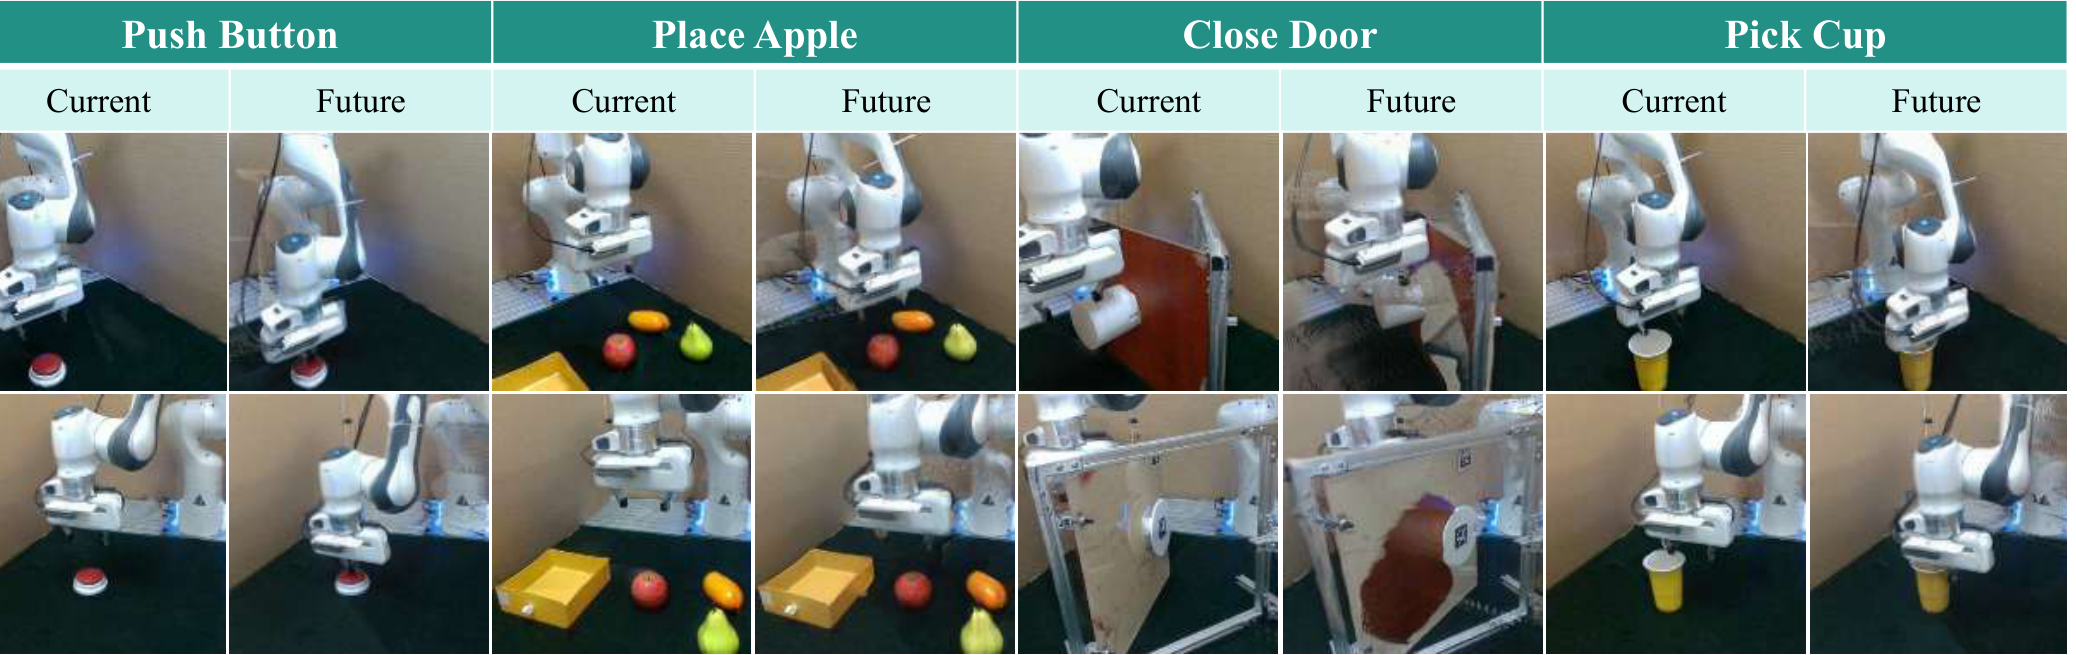
\includegraphics[width=0.9\linewidth,keepaspectratio]{figs/gaf_realworld.png}
   \caption{Real-world GAF results: renderings from current and predicted future Gaussians on four tasks \cite{p2}}
   \label{fig:gaf_real}
\end{figure}

\subsection{Discussion}

\paragraph{}
By embedding dynamics directly into an explicit scene representation, GAF closes the mismatch between static scene understanding and dynamic action generation. The predicted future Gaussians are not merely auxiliary supervision, as in prior Gaussian world models, but the very medium from which actions are extracted, producing a tight, interpretable coupling between prediction and control. The feed-forward design requires only sparse, unposed RGB views and runs in real time on a single GPU. Its principal limitation, acknowledged by the authors, is the absence of semantic or task-level understanding; incorporating language models to supply high-level priors is proposed as future work.

%---------------------------------------------------------------

\section{World Model-based Perception for Visual Legged Locomotion (WMP)}
This paper presents a simple yet effective end-to-end framework that combines Model-Based Reinforcement Learning (MBRL) world modeling with sim-to-real transfer for vision-based quadrupedal locomotion \cite{p3}. Instead of the two-stage privileged teacher--student paradigm, WMP builds a Recurrent State-Space Model (RSSM) of the environment in simulation and learns a policy directly on top of the world model's recurrent state, thereby avoiding both the information gap between teacher and student and the labor-intensive design of privileged observations.

\subsection{Problem Statement and Motivation}

\paragraph{} Reinforcement learning in simulation followed by sim-to-real transfer has produced robust legged locomotion. Blind policies that use only proprioception can walk over slopes and stairs, but terrains such as gaps and pits must be perceived \emph{in advance}, which requires vision. Learning directly from dense depth pixels with RL is extremely data-inefficient, and because a forward-facing camera cannot see beneath the robot, the policy must also remember past observations. The dominant solution is \textbf{privileged learning}: a teacher policy is trained with low-dimensional privileged information such as \emph{scandots} (terrain heights sampled around the robot), and a vision-based student policy is then trained to imitate it.

\paragraph{} Privileged learning has two limitations. First, the student cannot perfectly recover the teacher's behaviour, and the gap grows when the privileged information and images carry different information. Second, privileged information must be designed by hand for each terrain. As Figure~\ref{fig:wmp_scandots} shows, sparse scandots cannot resolve the precise distance to the walls of a narrow \emph{Tilt} passage and cannot represent off-ground obstacles such as the bar of a \emph{Crawl} obstacle, whereas depth images represent both. Inspired by the observation that animals learn to traverse terrain through an internal model of the world rather than privileged knowledge, WMP asks whether a learned world model can serve as the perception module.

\begin{figure}[htbp]
   \centering
   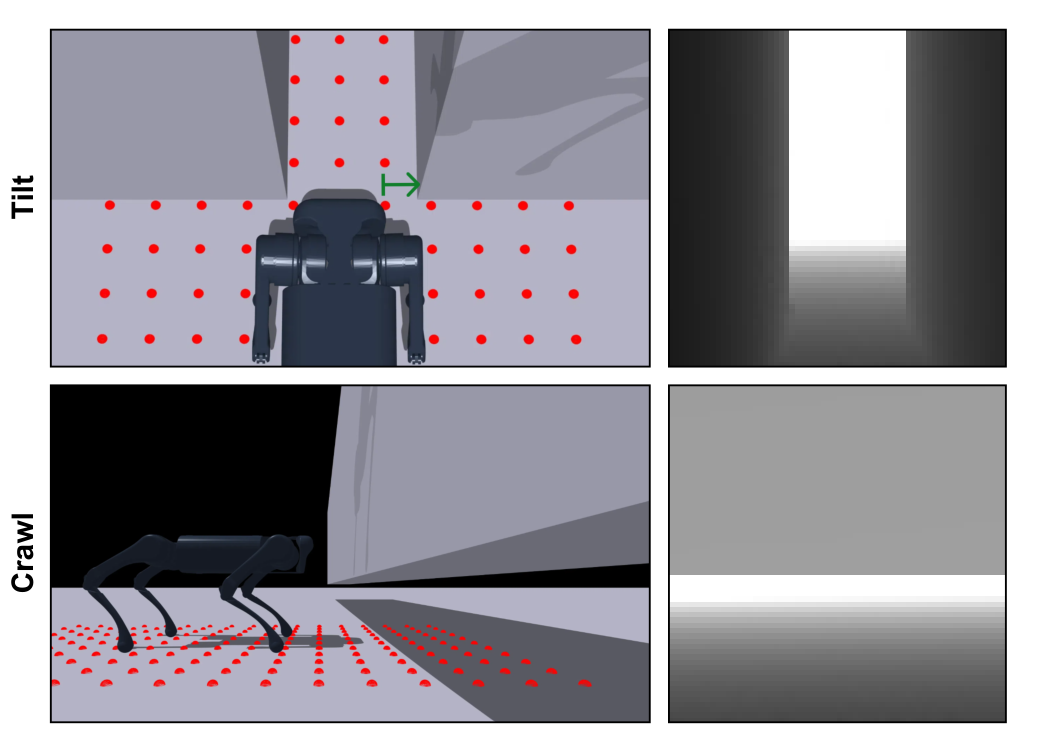
\includegraphics[width=0.42\linewidth,keepaspectratio]{figs/wmp_scandots.png}
   \caption{Scandots (left) and corresponding depth images (right) for Tilt and Crawl terrains: scandots cannot distinguish precise boundaries or represent off-ground obstacles \cite{p3}}
   \label{fig:wmp_scandots}
\end{figure}

\subsection{Problem Formulation}

\paragraph{} Locomotion is formulated as the POMDP of Equation~(\ref{eq:pomdp}). In vision-based locomotion the observation consists of proprioception $o^p_t$ and a depth image $d_t$, while the underlying state additionally contains privileged information $s^{\mathrm{pri}}_t$ available only in simulation:
\begin{equation}
o_t := (o^p_t,\, d_t),\qquad s_t := (o_t,\, s^{\mathrm{pri}}_t).
\end{equation}
The proprioception $o^p_t\in\mathbb{R}^{45}$ contains base angular velocity, projected gravity, velocity commands, joint positions and velocities, and the previous action. The depth image $d_t\in\mathbb{R}^{64\times64}$ has a $58^{\circ}\times58^{\circ}$ field of view. The privileged information contains scandots, foot contact forces, and randomized physical parameters. The action $a_t\in\mathbb{R}^{12}$ specifies joint position targets $q_d=q_{\mathrm{stand}}+a_t$, tracked by a PD controller:
\begin{equation}
\tau = K_p\,(q_d-q) + K_d\,(\dot{q}_d-\dot{q}),
\end{equation}
with $\dot{q}_d=0$ and $(K_p,K_d)=(40,\,1.0)$ on the real robot.

\subsection{World Model Learning}

\paragraph{} WMP adopts an RSSM variant (Section 2.4) with one important modification: because rendering depth images in simulation and running the RSSM on board are both expensive, the world model runs at a \emph{lower frequency} than the policy and updates its recurrent state only every $k$ time steps (Figure~\ref{fig:paper3_wm}). The four components are
\begin{align}
\text{Recurrent model:}\quad & h_t = f_\phi(h_{t-k},\, z_{t-k},\, a_{t-k:t-1}),\\
\text{Encoder:}\quad & z_t \sim q_\phi(\cdot\mid h_t,\, o_t),\\
\text{Dynamic predictor:}\quad & \hat{z}_t \sim p_\phi(\cdot\mid h_t),\\
\text{Decoder:}\quad & \hat{o}_t \sim p_\phi(\cdot\mid h_t,\, z_t).
\end{align}
The recurrent model is a GRU; the encoder and decoder use CNNs for the depth image and MLPs for proprioception. Note that the recurrent update consumes the whole action sequence $a_{t-k:t-1}$ executed since the last update. Following DreamerV3, the components are trained jointly on trajectory segments of length $L$ with the loss
\begin{equation}
\mathcal{L}(\phi)=\mathbb{E}_{q_\phi}\Big[\sum_{t=n\cdot k}^{L} -\ln p_\phi(o_t\mid z_t,h_t) + \beta\,\mathrm{KL}\big(q_\phi(\cdot\mid h_t,o_t)\,\|\,p_\phi(\cdot\mid h_t)\big)\Big],
\end{equation}
where $n$ is a non-negative integer. Predicting proprioception as well as depth encourages the model to capture physical properties of the environment.

\begin{figure}[htbp]
   \centering
   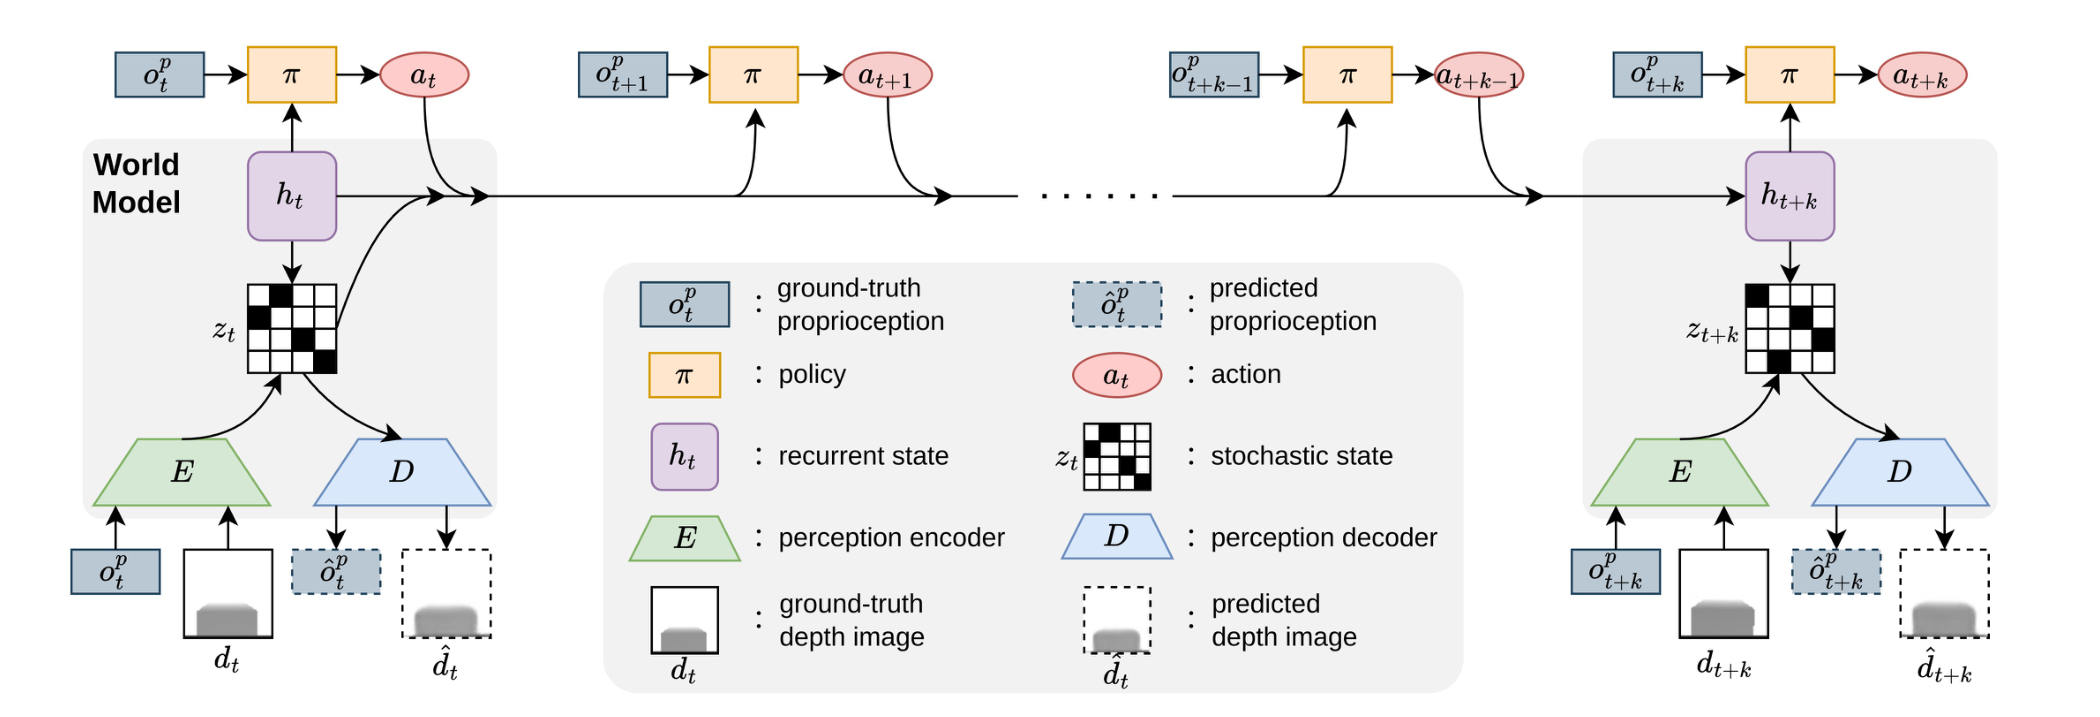
\includegraphics[width=0.92\linewidth,height=.26\textheight,keepaspectratio]{wmp_framework.png}
   \caption{The WMP framework: the RSSM world model runs every $k$ steps and its recurrent state feeds the policy \cite{p3}}
   \label{fig:paper3_wm}
\end{figure}

\subsection{Policy Learning}

\paragraph{} The key insight of WMP is that the recurrent state $h_t$ of a well-trained world model contains enough information to predict the future and is therefore akin to the underlying Markovian state. The policy takes $h_t$ as input together with the current proprioception, for every step between two world-model updates:
\begin{equation}
a_{t+i}\sim\pi_\theta\big(\cdot\mid o^p_{t+i},\,\mathrm{sg}(h_t)\big),\qquad \forall i\in[0,k-1],
\end{equation}
where $\mathrm{sg}(\cdot)$ is the stop-gradient operator, so policy gradients do not alter the world model. An \textbf{asymmetric actor--critic} is used, in which the critic additionally observes the privileged information:
\begin{equation}
v(s_{t+i})\sim V_\theta\big(\cdot\mid o^p_{t+i},\,\mathrm{sg}(h_t),\,s^{\mathrm{pri}}_{t+i}\big).
\end{equation}
The authors find that $h_t$ is essential even for the critic, because scandots cannot represent Tilt and Crawl terrains. Actor and critic are trained with PPO on simulator data. Unlike Dreamer-style MBRL, WMP does \emph{not} train the policy on imagined rollouts: since the world model is itself trained on simulator data, it cannot be more accurate than the simulator, and sampling from the parallel simulator is already cheap.

\subsection{Training Environment and Rewards}

\paragraph{} Training uses the \texttt{legged\_gym} codebase on the Isaac Gym simulator with 4096 parallel Unitree A1 robots on six terrain types---Slope, Stair, Gap, Climb, Tilt, and Crawl---with increasing difficulty levels and the terrain curriculum of Rudin et al.: a robot is promoted when it crosses its terrain and demoted when it travels less than half the commanded distance. The policy acts at 50 Hz (0.02 s per step); depth images are computed every $k$ steps and delivered with a 100 ms latency to aid transfer, and physical parameters are randomized.

\paragraph{} The robot tracks a command $(v^{\mathrm{cmd}}_x,v^{\mathrm{cmd}}_y,\omega^{\mathrm{cmd}}_z)$. Instead of hand-selected waypoints, a simple clipped velocity-tracking reward is used,
\begin{equation}
r_{\mathrm{tracking}}=\exp\!\Big(-\big(\min(v_{xy},\,v^{\mathrm{cmd}}_{xy}+0.1)-v^{\mathrm{cmd}}_{xy}\big)^2/\sigma\Big),
\end{equation}
which lets the robot exceed the commanded speed when necessary, for example to jump a gap. Penalties discourage getting stuck or turning around obstacles, and an Adversarial Motion Priors (AMP) style reward encourages natural gaits:
\begin{equation}
r_{\mathrm{style}}(s,s')=\max\!\big[0,\;1-0.25\,(D_\psi(s,s')-1)^2\big],
\end{equation}
where the discriminator $D_\psi$ is trained with a least-squares objective and gradient penalty to distinguish state transitions from a reference motion dataset from those produced by the policy.

\subsection{Simulation Results}

\paragraph{} WMP is compared with a \textbf{Teacher} (oracle with scandots), a \textbf{Student} reproduced from Cheng et al.\ (ConvNet-RNN imitating the teacher from depth), a \textbf{Blind} ablation without depth, and \textbf{WMP w/o Prop} without proprioception in the world model. Table~\ref{tab:wmp_sim} and Figure~\ref{fig:wmp_chart} report returns and velocity tracking errors averaged over 100 trajectories. WMP attains near-teacher returns on all terrains where the teacher is applicable (e.g.\ 32.37 vs.\ 32.80 on Gap) while the student falls far behind (27.07). Removing depth collapses performance on every terrain except Slope, and removing proprioception degrades performance slightly. Teacher and Student are not applicable to Tilt and Crawl because scandots cannot describe these terrains.

{\renewcommand{\arraystretch}{1.2}
\begin{table}[htbp]
\centering
\caption{Simulation comparison of WMP (return $\uparrow$ / velocity tracking error $\downarrow$), mean over 100 trajectories \cite{p3}}\label{tab:wmp_sim}
\footnotesize
\setlength{\tabcolsep}{3.5pt}
\begin{tabular}{|l|l|c|c|c|c|c|c|}
\hline
 & \textbf{Method} & \textbf{Slope} & \textbf{Stair} & \textbf{Gap} & \textbf{Climb} & \textbf{Tilt} & \textbf{Crawl} \\ \hline
\multirow{5}{*}{Return} & WMP (ours) & \textbf{36.55} & \textbf{35.06} & \textbf{32.37} & 34.64 & \textbf{34.73} & \textbf{36.60} \\ \cline{2-8}
 & Teacher (oracle) & 36.70 & 35.07 & 32.80 & 35.32 & N/A & N/A \\ \cline{2-8}
 & Student & 36.31 & 34.93 & 27.07 & 33.42 & N/A & N/A \\ \cline{2-8}
 & Blind & 33.96 & 23.56 & 9.80 & 14.11 & 3.94 & 8.92 \\ \cline{2-8}
 & WMP w/o Prop & 36.07 & 34.62 & 30.73 & \textbf{34.67} & 30.78 & 36.41 \\ \hline
\multirow{5}{*}{\shortstack[l]{Tracking\\error}} & WMP (ours) & \textbf{0.008} & \textbf{0.013} & \textbf{0.26} & \textbf{0.13} & \textbf{0.02} & \textbf{0.006} \\ \cline{2-8}
 & Teacher (oracle) & 0.007 & 0.012 & 0.23 & 0.09 & N/A & N/A \\ \cline{2-8}
 & Student & 0.008 & 0.015 & 0.35 & 0.16 & N/A & N/A \\ \cline{2-8}
 & Blind & 0.019 & 0.033 & 0.33 & 0.26 & 0.08 & 0.051 \\ \cline{2-8}
 & WMP w/o Prop & 0.009 & 0.017 & 0.28 & 0.14 & 0.08 & 0.013 \\ \hline
\end{tabular}
\end{table}}

\begin{figure}[htbp]
\centering
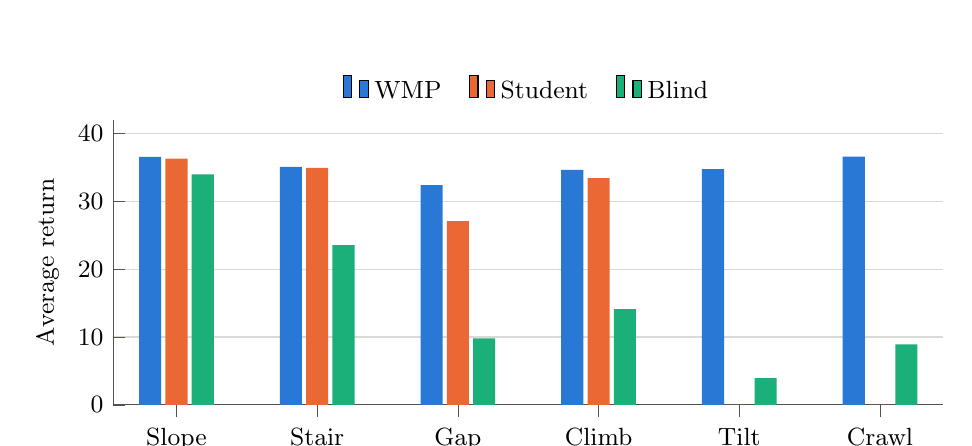
\begin{tikzpicture}
\begin{axis}[
  ybar=1.5pt, bar width=8pt, width=\textwidth, height=5.2cm,
  symbolic x coords={Slope,Stair,Gap,Climb,Tilt,Crawl}, xtick=data, enlarge x limits=0.09,
  ymin=0, ymax=42, ylabel={Average return}, ylabel style={font=\small},
  ymajorgrids, grid style={gridgray}, axis line style={inkgray}, tick style={inkgray},
  axis x line*=bottom, axis y line*=left, tick label style={font=\small},
  legend style={at={(0.5,1.02)}, anchor=south, legend columns=-1, draw=none, font=\small, /tikz/every even column/.append style={column sep=8pt}},
]
\addplot[fill=seriesA, draw=none] coordinates {(Slope,36.55) (Stair,35.06) (Gap,32.37) (Climb,34.64) (Tilt,34.73) (Crawl,36.60)};
\addplot[fill=seriesB, draw=none] coordinates {(Slope,36.31) (Stair,34.93) (Gap,27.07) (Climb,33.42) (Tilt,0) (Crawl,0)};
\addplot[fill=seriesC, draw=none] coordinates {(Slope,33.96) (Stair,23.56) (Gap,9.80) (Climb,14.11) (Tilt,3.94) (Crawl,8.92)};
\legend{WMP, Student, Blind}
\end{axis}
\end{tikzpicture}
\caption{Simulated returns of WMP, the privileged-learning Student, and the Blind ablation on six terrains, plotted from \cite{p3}. The Student is not applicable to Tilt and Crawl (no bar).}
\label{fig:wmp_chart}
\end{figure}

\subsection{Empirical Analysis of the World Model}

\paragraph{} \textbf{Recurrent state visualization.} A t-SNE projection of $h_t$ collected on the six terrains (Figure~\ref{fig:wmp_analysis}, left) shows clearly separated clusters, with only slight overlap between Slope and Climb, whose depth images are similar (a climb is essentially a $90^{\circ}$ slope). The recurrent state therefore encodes terrain type without any explicit supervision.

\paragraph{} \textbf{Model interval and training length.} Varying $k$ from 2 to 30 shows that smaller intervals yield higher simulated returns because the robot reacts faster (Figure~\ref{fig:wmp_analysis}, right). On the real A1, however, acquiring a depth image and running the world model takes about 40 ms, so $k=5$ (0.1 s) is chosen as a trade-off. Training segments of about one second already give acceptable performance---intuitively, what the robot saw a second ago is roughly under its feet---while very long segments make back-propagation through the RSSM inefficient; 6.4 s segments are used in the main experiments.

\begin{figure}[htbp]
\centering
\begin{subfigure}[b]{0.32\textwidth}
  \centering
  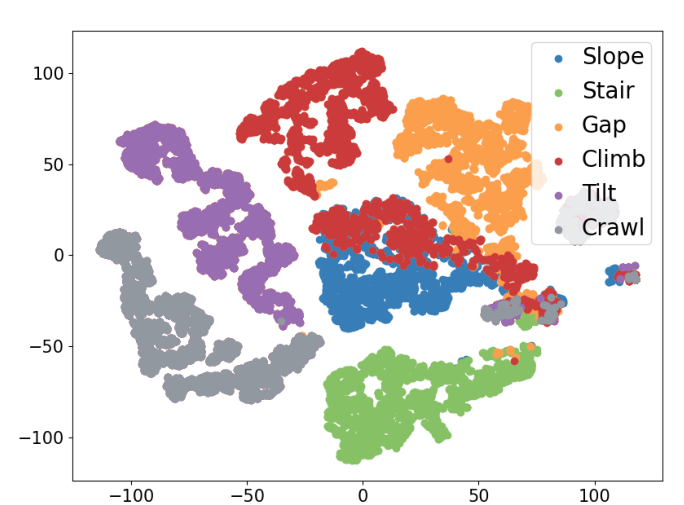
\includegraphics[width=\linewidth,keepaspectratio]{figs/wmp_tsne.png}
  \caption{t-SNE of $h_t$}
\end{subfigure}\hfill
\begin{subfigure}[b]{0.66\textwidth}
  \centering
  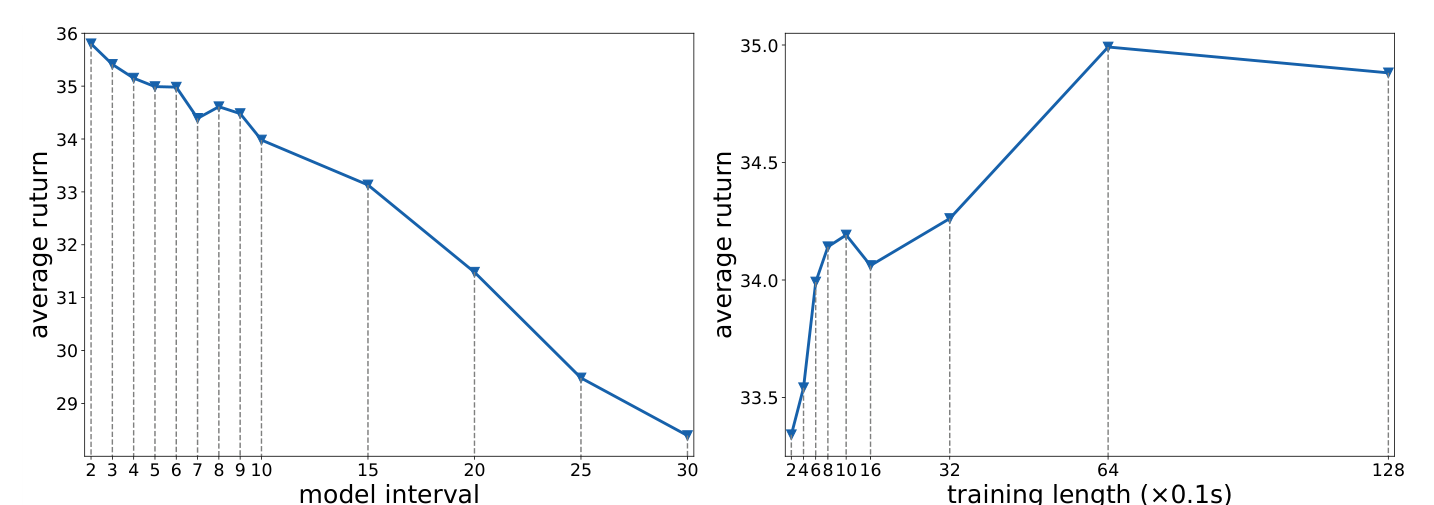
\includegraphics[width=\linewidth,keepaspectratio]{figs/wmp_interval.png}
  \caption{Return vs.\ model interval $k$ and training length}
\end{subfigure}
\caption{Empirical study of the WMP world model \cite{p3}}
\label{fig:wmp_analysis}
\end{figure}

\paragraph{} \textbf{Real-world prediction.} Given only the initial observation and the executed action sequence, the world model trained purely in simulation predicts real depth sequences accurately, especially at the critical location the robot is about to traverse (Figure~\ref{fig:wmp_pred}). For the Crawl obstacle the predicted shape differs from reality because such shapes never appeared in simulation, yet the position and angle of the traversable crevice are consistent---evidence that latent-space world modelling generalizes and helps explain WMP's smooth sim-to-real transfer.

\begin{figure}[htbp]
   \centering
   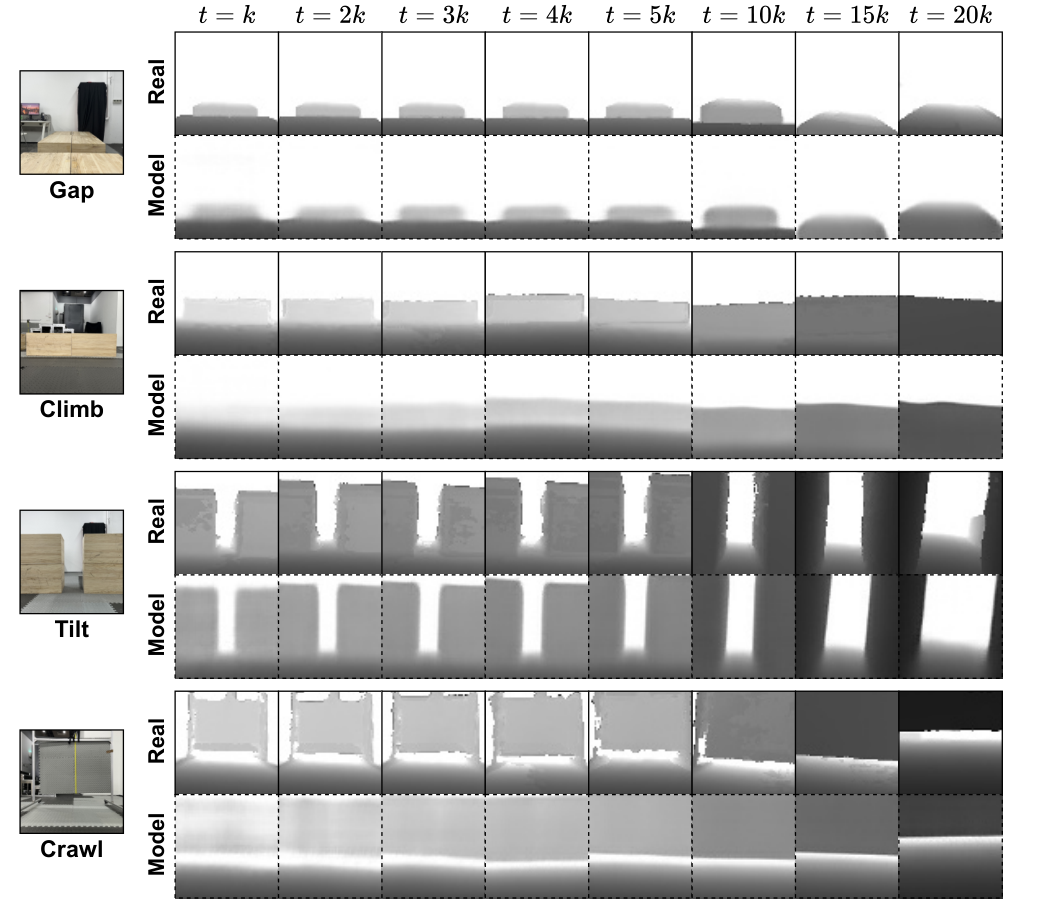
\includegraphics[width=0.48\linewidth,keepaspectratio]{figs/wmp_prediction.png}
   \caption{Real-world depth images and long-horizon predictions of the WMP world model on Gap, Climb, Tilt, and Crawl \cite{p3}}
   \label{fig:wmp_pred}
\end{figure}

\subsection{Real-World Evaluation}

\paragraph{} All policies run on the A1's onboard Jetson NX. Depth from the front RealSense D435i is read at 60 Hz ($424\times240$), filtered spatially and temporally to reduce noise, cropped and down-sampled to $64\times64$, and fed to the world model with 100 ms latency. Five terrains of increasing difficulty are tested over ten trials each (Figure~\ref{fig:wmp_real}). The Student succeeds on easy Stair, Gap, and Climb settings but fails at harder levels and cannot handle Tilt or Crawl at all. WMP traverses a Gap of 85 cm (about 2.1$\times$ body length), a Climb of 55 cm (about 2.2$\times$ robot height), and a Crawl clearance of 22 cm (about 0.8$\times$ robot height), close to the hardest simulated levels and the best reported traversal performance on the A1. Ablating proprioception or images degrades performance. Outdoor deployment in a park shows consistent behaviour: the robot climbs stairs, mounts platforms up to 45 cm, and traverses grass and gravel.

\begin{figure}[htbp]
   \centering
   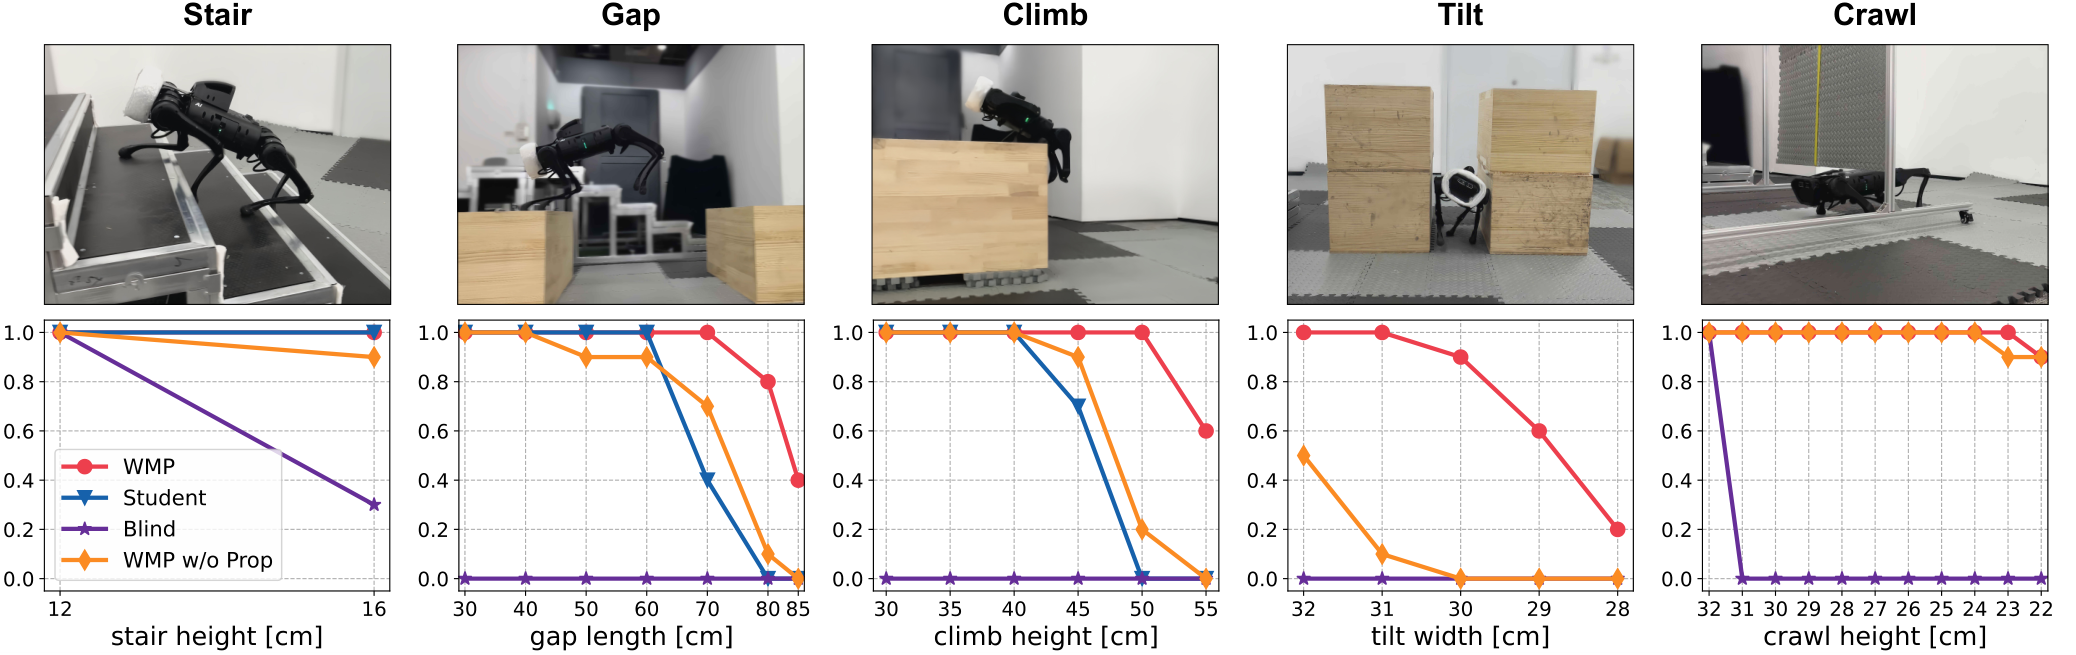
\includegraphics[width=0.92\linewidth,keepaspectratio]{figs/wmp_realworld.png}
   \caption{Real-world success rates of WMP, Student, Blind, and WMP w/o Prop over ten trials per difficulty level \cite{p3}}
   \label{fig:wmp_real}
\end{figure}

\subsection{Discussion}

\paragraph{}
WMP demonstrates that a world model trained entirely in simulation can serve as a transferable perceptual front-end for real robots: the recurrent state compresses a history of high-dimensional depth images into an informative, terrain-discriminative representation. This single-stage alternative to privileged learning removes teacher--student performance gaps and generalizes across terrains that hand-designed privileged observations cannot represent. Its limitations are that the model cannot exceed the simulator's fidelity, that hardware latency forces a coarse model interval, and that long training segments are inefficient to back-propagate. The authors suggest training the world model on a mixture of simulated and real data and adding modalities such as touch.

%---------------------------------------------------------------

\section{WMNav: Integrating Vision-Language Models into World Models for Object Goal Navigation}
This study proposes a fully modular, training-free world-model framework for Zero-Shot Object Navigation (ZSON), in which Vision-Language Models (VLMs) carry out all perception, prediction, planning, and reasoning \cite{p4}. Instead of interacting with the environment to discover the target by trial and error, the agent imagines the likely outcome of each direction of travel---exploiting the commonsense knowledge of indoor layouts embedded in VLMs---and stores these predictions in an online memory that steers exploration.

\subsection{Problem Statement and Motivation}

\paragraph{} In object goal navigation, an agent placed in an unseen indoor environment must find and stop near an instance of a given category (e.g.\ \emph{bed}, \emph{sofa}, \emph{toilet}). In the zero-shot setting the categories and environments are not seen during training. Existing methods are either \emph{network-based}, training policies with RL or IL on large datasets, or \emph{map-based}, building semantic maps and choosing frontiers or waypoints; the latter depend on accurate, complex map construction and do not fully exploit VLMs trained on egocentric images. Most importantly, both kinds of methods must actually interact with the environment to understand it, rather than anticipating the outcomes of their choices. VLFM builds a value map of target likelihood using BLIP-2, but its limited reasoning makes complex planning difficult. Humans, by contrast, can imagine a room layout from visual cues and common design patterns---walking along a corridor usually leads to new rooms, and searching a bathroom for a sofa is unwise. WMNav hypothesizes that VLMs, trained on vast amounts of first-person imagery, have acquired enough commonsense to play the role of such a world model (Figure~\ref{fig:wmnav_intro}).

\begin{figure}[htbp]
   \centering
   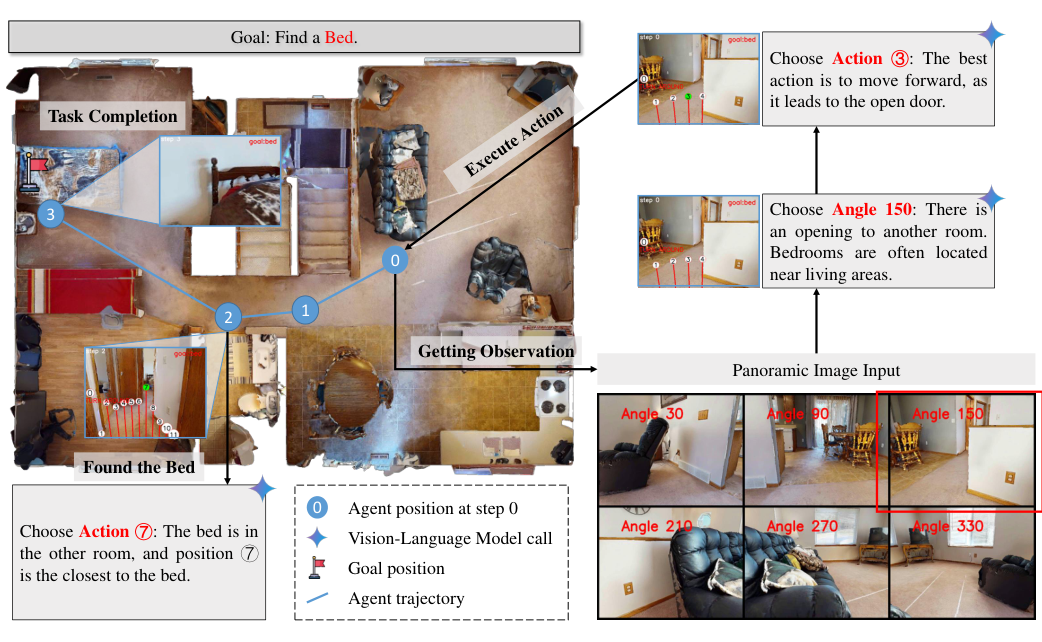
\includegraphics[width=0.55\linewidth,keepaspectratio]{figs/wmnav_intro.png}
   \caption{World model navigation with a VLM: the model estimates the goal's likelihood in each panoramic direction, plans an intermediate subtask, and selects an action \cite{p4}}
   \label{fig:wmnav_intro}
\end{figure}

\subsection{Task Definition and Framework Overview}

\paragraph{} At each step $t$ the agent receives an RGB-D observation $O_t$ and its pose $P_t$ and chooses an action. Instead of the usual discrete action set \{Stop, Move Forward, Turn Left, Turn Right, Look Up, Look Down\}, WMNav uses polar-coordinate actions $a_t=(r_t,\theta_t)$ specifying a direction and a distance. An episode succeeds if the agent stops within a threshold distance $d_{\mathrm{thres}}$ of a goal instance.

\paragraph{} The framework (Figure~\ref{fig:paper4_wm}) begins by rotating the agent through the six headings $\mathcal{A}=\{30^{\circ}, 90^{\circ}, \ldots, 330^{\circ}\}$ (in steps of $60^{\circ}$) to capture six RGB-D images forming a panorama $I^{\mathrm{pan}}_t$. The \textbf{world model} comprises a PredictVLM together with a memory built from the Curiosity Value Map and a cost; it receives no reward from the environment and is used only to predict and simplify the future state of the world. The \textbf{navigation policy} comprises a PlanVLM and a ReasonVLM, whose prompts are configured by the cost, so that the policy is optimized through prompting without fine-tuning any VLM.

\begin{figure}[htbp]
   \centering
   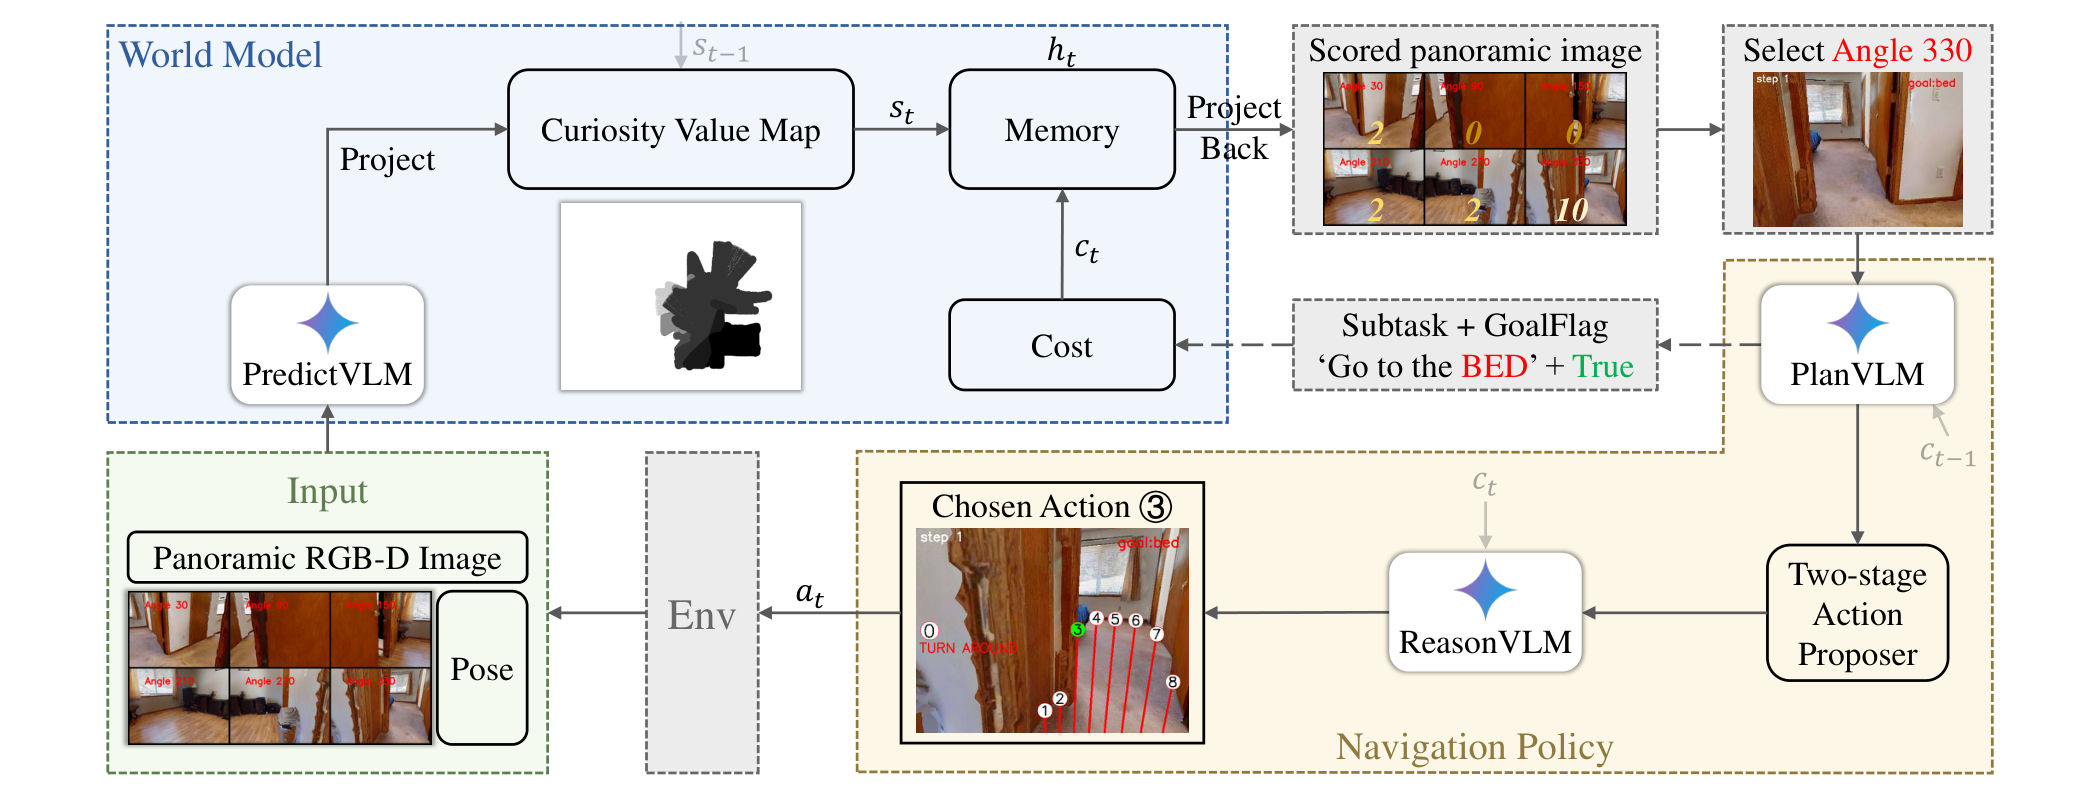
\includegraphics[width=0.92\linewidth,height=.26\textheight,keepaspectratio]{wmnav_framework.png}
   \caption{The WMNav framework with VLM-based world model and navigation policy \cite{p4}}
   \label{fig:paper4_wm}
\end{figure}

\subsection{World Model: Prediction and Curiosity Value Map}

\paragraph{} \textbf{VLM-based state prediction.} The panoramic image is given to PredictVLM with a structured prompt asking it to score every direction from 0 to 10: a direction with no feasible path and no target scores 0, a direction in which the goal is visible scores 10, and intermediate cases receive intermediate scores, each with a textual explanation returned in JSON format:
\begin{equation}
\mathrm{Score}_t = \mathrm{PredictVLM}\big(I^{\mathrm{pan}}_t\big).
\end{equation}

\paragraph{} \textbf{Curiosity Value Map construction.} The Curiosity Value Map $M^{cv}$ is a top-down grid in which each cell stores the curiosity value of that location (0--10). Cells are initialized to 10, since at the start the target could be anywhere. At each step the scores are projected from the egocentric navigable areas onto a top-down map $M^{nav}_t$ using depth $D_t$ and pose $P_t$, and fused with the previous map by a pixel-wise minimum:
\begin{equation}
M^{nav}_t=\mathrm{Projection}(\mathrm{Score}_t),\qquad M^{cv}_t(u,v)=\min\big(M^{cv}_{t-1}(u,v),\;M^{nav}_t(u,v)\big).
\end{equation}
The minimum ensures that regions already observed to lack the goal (score 0) stay suppressed, preventing redundant back-and-forth exploration (Figure~\ref{fig:wmnav_cvm}).

\begin{figure}[htbp]
   \centering
   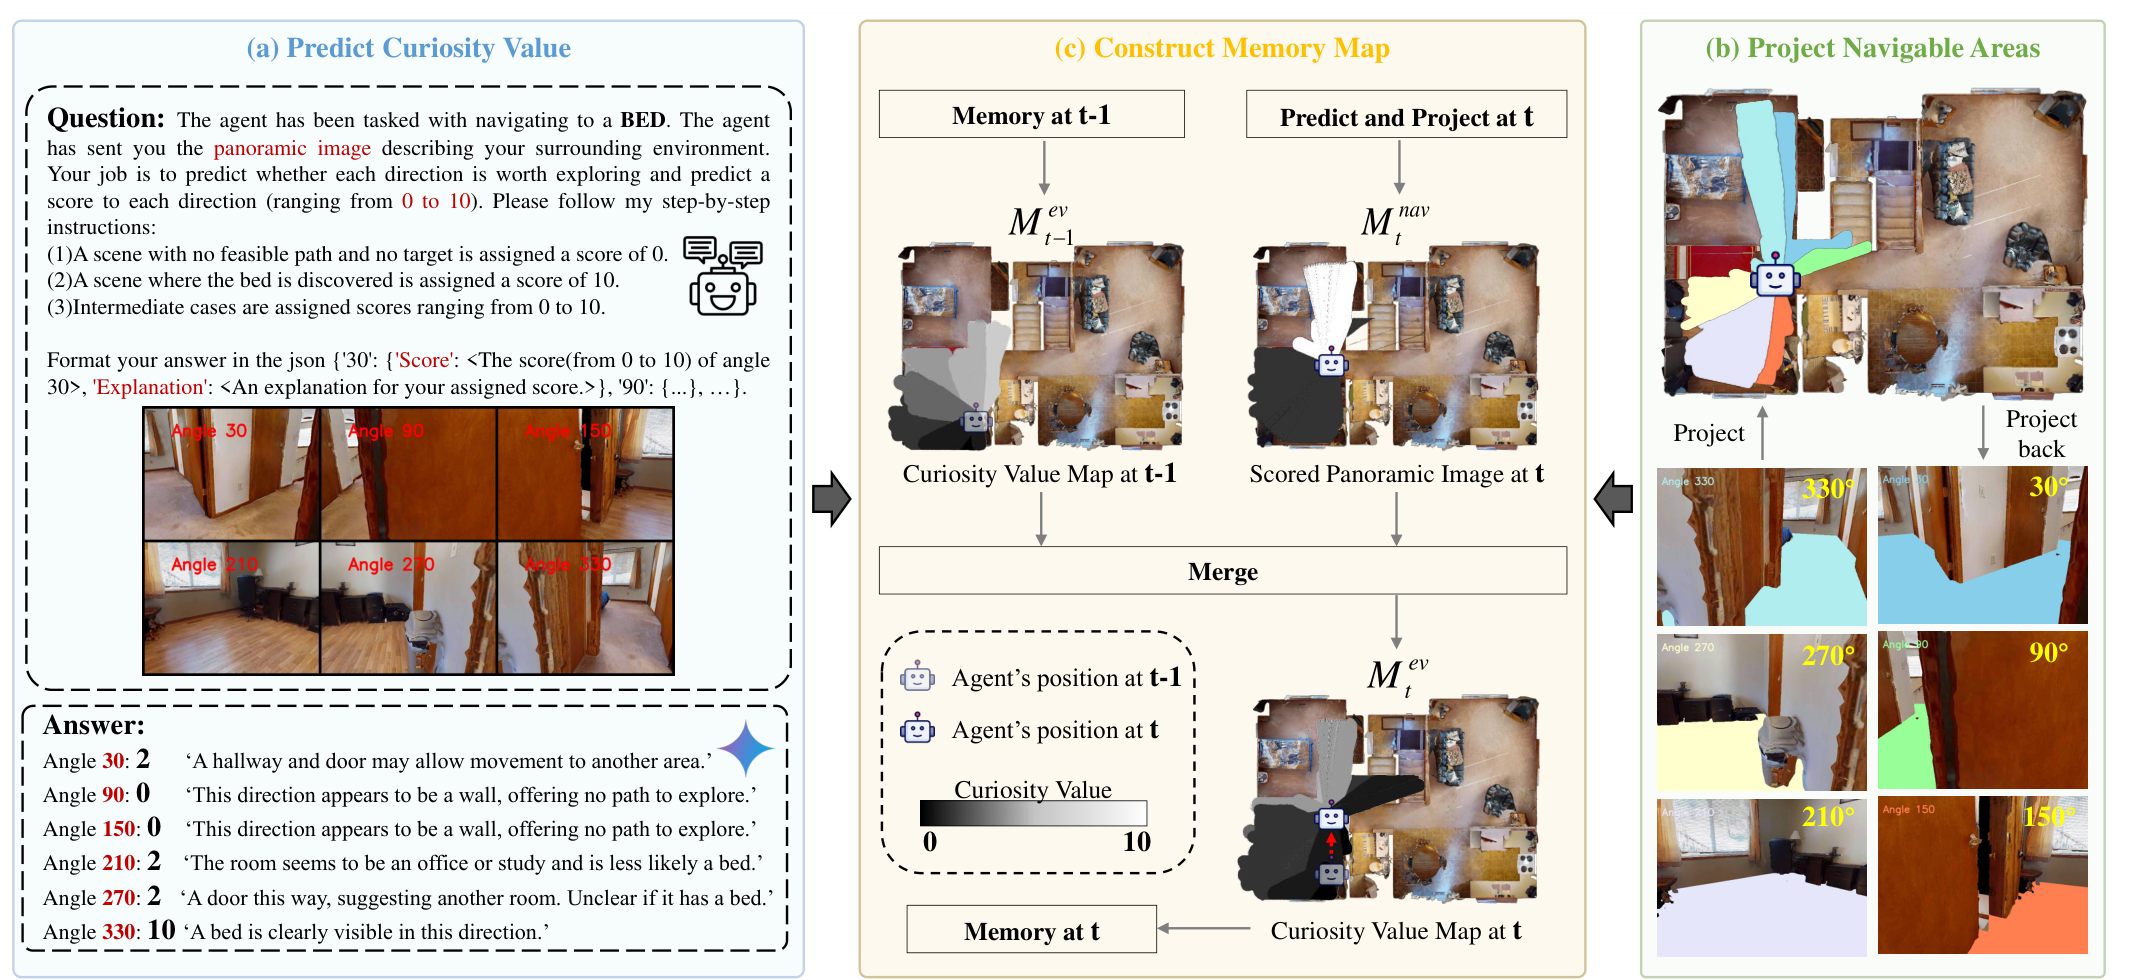
\includegraphics[width=0.92\linewidth,keepaspectratio]{figs/wmnav_curiosity.png}
   \caption{(a) Predicting curiosity values for each panoramic direction; (b) projection of navigable areas between egocentric and top-down views; (c) fusing predictions into the Curiosity Value Map \cite{p4}}
   \label{fig:wmnav_cvm}
\end{figure}

\paragraph{} \textbf{Cost.} Because a VLM world model receives no environmental reward, WMNav defines a \emph{cost} consisting of the current subtask and a goal flag indicating whether the goal has been seen. The cost is inserted into the prompts of PlanVLM and ReasonVLM, implicitly optimizing the policy's outputs. The memory $h_t$ therefore consists of the map $s_t$ and the cost $c_t$.

\subsection{Subtask Decomposition}

\paragraph{} Planning directly towards an unseen goal provides very sparse feedback. WMNav therefore decomposes the goal into intermediate subtasks, as a human would: find the corridor to the bedroom, reach the bedroom door, then approach the bed. After the map update, curiosity values are projected back onto the current navigable areas, the average score of each direction is computed, and the direction $\alpha$ with the highest score is selected. Its image $I_t(\alpha)$, the explanation for choosing it, and the previous subtask are given to PlanVLM, which outputs a new subtask and goal flag:
\begin{equation}
\mathrm{SubTask}_t,\;\mathrm{GoalFlag}_t=\mathrm{PlanVLM}\big(I_t(\alpha),\,\mathrm{SubTask}_{t-1}\big).
\end{equation}
Comparing the plan with the new observation provides feedback that mitigates hallucination: if the previous subtask is not complete, the agent continues it; if it is complete, a new one is chosen.


\subsection{Two-Stage Action Proposer}

\paragraph{} Candidate actions are generated following VLMNav: $K$ polar vectors are sampled at regular angular intervals $\Delta\theta$ within the navigable area of $I_t(\alpha)$, giving $A^{\mathrm{init}}_t=\{(r_{t,i},\theta_{t,i})\}_{i=1}^{K}$. Actions leading into already-explored regions are filtered out using an exploration state map, distances and angular spacing are constrained, and the remaining $K'$ candidates $A^{\mathrm{cand}}_t$ are drawn as numbered arrows on the image to produce $I^{\mathrm{ann}}_t$ (Figure~\ref{fig:wmnav_action}). Decision making is split into two stages:
\begin{itemize}
  \item \textbf{Exploration stage:} ReasonVLM, configured as ActionVLM, chooses the candidate that best serves the current subtask:
  \begin{equation}
  a_t=\mathrm{ReasonVLM}\big(\mathrm{SubTask}_t,\,\mathrm{Goal}_t,\,I^{\mathrm{ann}}_t\big),\qquad a_t=(r_t,\theta_t).
  \end{equation}
  \item \textbf{Goal-approaching stage:} once the goal is detected, the length constraint is removed and sampling becomes denser so that some vector ends at the goal's ground location; ReasonVLM, configured as GoalVLM, selects it. Rather than trusting the VLM to decide when to stop, stopping is triggered geometrically:
  \begin{equation}
  \mathrm{StopFlag}=\begin{cases}\text{True}, & \mathrm{DistanceToGoal}<d_{\mathrm{thres}}\\ \text{False}, & \text{otherwise.}\end{cases}
  \end{equation}
\end{itemize}

\begin{figure}[htbp]
   \centering
   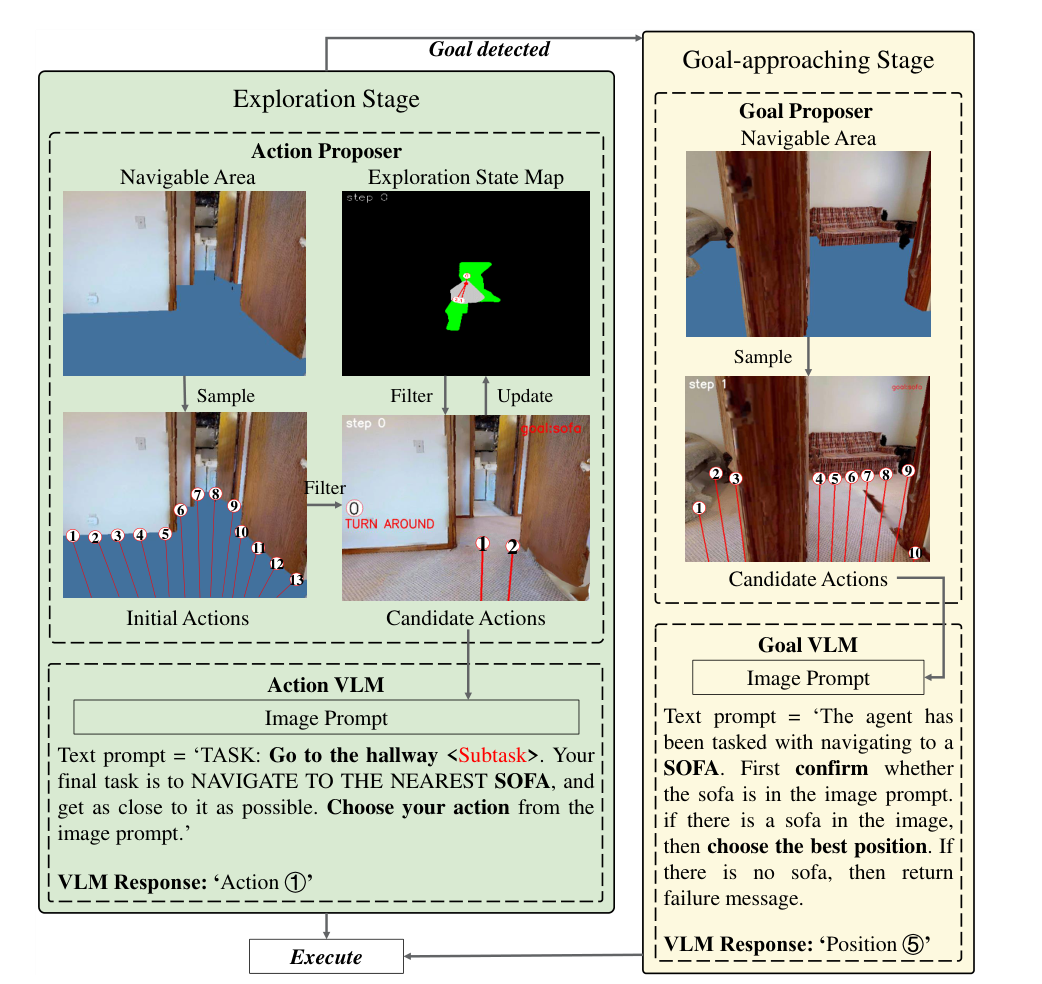
\includegraphics[width=0.5\linewidth,keepaspectratio]{figs/wmnav_action.png}
   \caption{Reasoning the action: the exploration stage filters sampled actions for ActionVLM, and the goal-approaching stage densely samples positions for GoalVLM \cite{p4}}
   \label{fig:wmnav_action}
\end{figure}

\subsection{Experimental Setup}

\paragraph{} WMNav is evaluated in the Habitat simulator on three benchmarks: \textbf{HM3D v0.1} (2000 validation episodes in 20 environments, 6 goal categories; used in the Habitat 2022 ObjectNav challenge), \textbf{HM3D v0.2} (1000 validation episodes with improved geometry and semantic labels), and \textbf{MP3D} (11 scenes, 2195 validation episodes, 21 goal categories). Metrics are SR and SPL (Equation~\ref{eq:spl}). Table~\ref{tab:wmnav_setup} lists the agent configuration; Gemini VLMs are used by default for their low cost and high effectiveness.

{\renewcommand{\arraystretch}{1.2}
\begin{table}[htbp]
\centering
\caption{Agent configuration used in WMNav experiments \cite{p4}}\label{tab:wmnav_setup}
\small
\begin{tabularx}{\textwidth}{|p{5cm}|X|}
\hline
\textbf{Parameter} & \textbf{Value} \\ \hline
Maximum navigation steps & 40 \\ \hline
Agent body & Cylinder, radius 0.18 m, height 0.88 m \\ \hline
Camera & Egocentric RGB-D, $640\times480$, horizontal FoV $79^{\circ}$, pitched down $14^{\circ}$ \\ \hline
Panorama headings & $30^{\circ},90^{\circ},150^{\circ},210^{\circ},270^{\circ},330^{\circ}$ \\ \hline
Success threshold $d_{\mathrm{thres}}$ & 1.0 m \\ \hline
VLMs & Gemini series (default); Qwen2.5-VL in ablations \\ \hline
Training & None (training-free, zero-shot; no detectors or pre-built maps) \\ \hline
\end{tabularx}
\end{table}}

\subsection{Results and Analysis}

\paragraph{} \textbf{Comparison with the state of the art.} Table~\ref{tab:wmnav_sota} compares WMNav with supervised and zero-shot methods. WMNav outperforms all zero-shot methods, improving SR by 3.2 points and SPL by 3.2 points on HM3D and SR by 13.5 points and SPL by 1.1 points on MP3D over the previous best. Even including supervised methods, it achieves the best SR on MP3D and the best SPL on HM3D. The authors argue that LLM-based methods such as ESC lose spatial detail when converting images to text; detector-based semantic maps (OpenFMNav) are complex and under-use the VLM; top-view inputs (TopV-Nav) do not exploit VLMs' egocentric training; whereas the simple Curiosity Value Map directly exploits the VLM's egocentric scene understanding.

{\renewcommand{\arraystretch}{1.25}
\begin{table}[htbp]
\centering
\caption{Object navigation results on HM3D v0.1 and MP3D. TF: training-free; ZS: zero-shot \cite{p4}}\label{tab:wmnav_sota}
\small
\begin{tabular}{|l|c|c|c|c|c|c|}
\hline
\multirow{2}{*}{\textbf{Method}} & \multirow{2}{*}{\textbf{TF}} & \multirow{2}{*}{\textbf{ZS}} & \multicolumn{2}{c|}{\textbf{HM3D}} & \multicolumn{2}{c|}{\textbf{MP3D}} \\ \cline{4-7}
 & & & SR (\%) & SPL (\%) & SR (\%) & SPL (\%) \\ \hline
Habitat-Web & $\times$ & $\times$ & 41.5 & 16.0 & 31.6 & 8.5 \\ \hline
OVRL & $\times$ & $\times$ & -- & -- & 28.6 & 7.4 \\ \hline
OVRL-V2 & $\times$ & $\times$ & 64.7 & 28.1 & -- & -- \\ \hline
ZSON & $\times$ & \checkmark & 25.5 & 12.6 & 15.3 & 4.8 \\ \hline
PSL & $\times$ & \checkmark & 42.4 & 19.2 & 18.9 & 6.4 \\ \hline
PixNav & $\times$ & \checkmark & 37.9 & 20.5 & -- & -- \\ \hline
SGM & $\times$ & \checkmark & 60.2 & 30.8 & 37.7 & 14.7 \\ \hline
VLFM & $\times$ & \checkmark & 52.5 & 30.4 & 36.4 & 17.5 \\ \hline
CoW & \checkmark & \checkmark & -- & -- & 9.2 & 4.9 \\ \hline
ESC & \checkmark & \checkmark & 39.2 & 22.3 & 28.7 & 14.2 \\ \hline
L3MVN & \checkmark & \checkmark & 50.4 & 23.1 & -- & -- \\ \hline
VoroNav & \checkmark & \checkmark & 42.0 & 26.0 & -- & -- \\ \hline
OpenFMNav & \checkmark & \checkmark & 54.9 & 24.4 & -- & -- \\ \hline
TopV-Nav & \checkmark & \checkmark & 45.9 & 28.0 & 31.9 & 16.1 \\ \hline
\textbf{WMNav (ours)} & \checkmark & \checkmark & \textbf{58.1} & \textbf{31.2} & \textbf{45.4} & \textbf{17.2} \\ \hline
\end{tabular}
\end{table}}

\paragraph{} \textbf{Ablation of modules and memory.} Table~\ref{tab:wmnav_abl} shows ablations on HM3D v0.2. Adding subtask decomposition (a$\rightarrow$b), the Curiosity Value Map (a$\rightarrow$d), and the two-stage action proposer (e$\rightarrow$f) each improves SR, reaching 72.2\% with all modules. Among memory strategies, a \emph{text--image} memory, in which the VLM describes observations in text and plans over a top-down trajectory map, performs even worse than no memory, because feeding the VLM text--image combinations easily induces hallucinations. The quantitative Curiosity Value Map forces rigorous outputs and gives the best SR and SPL.

{\renewcommand{\arraystretch}{1.25}
\begin{table}[htbp]
\centering
\caption{Ablation of modules and memory strategies on HM3D v0.2. SD: subtask decomposition; TAP: two-stage action proposer; CVM: Curiosity Value Map \cite{p4}}\label{tab:wmnav_abl}
\small
\begin{tabular}{|c|l|c|c|c|c|}
\hline
 & \textbf{Memory} & \textbf{SD} & \textbf{TAP} & \textbf{SR (\%)} & \textbf{SPL (\%)} \\ \hline
a & No memory & $\times$ & $\times$ & 65.8 & 25.8 \\ \hline
b & No memory & \checkmark & $\times$ & 67.4 & 33.1 \\ \hline
c & Text--image & \checkmark & $\times$ & 62.0 & 29.6 \\ \hline
d & CVM & $\times$ & $\times$ & 69.5 & \textbf{34.9} \\ \hline
e & CVM & \checkmark & $\times$ & 70.1 & 34.7 \\ \hline
f & CVM & \checkmark & \checkmark & \textbf{72.2} & 33.3 \\ \hline
\end{tabular}
\end{table}}

\paragraph{} \textbf{Effect of the VLM.} When every VLM in the framework is replaced by the same model (Figure~\ref{fig:wmnav_chart}), performance increases with model scale---Qwen2.5-VL-3B reaches 29.7\% SR and the 7B model 46.1\%---and proprietary Gemini models perform best, with Gemini 1.5 Pro reaching 58.1\% SR and 31.2\% SPL. Even Gemini 1.5 Flash (53.5\% SR) remains competitive with prior methods.

\begin{figure}[htbp]
\centering
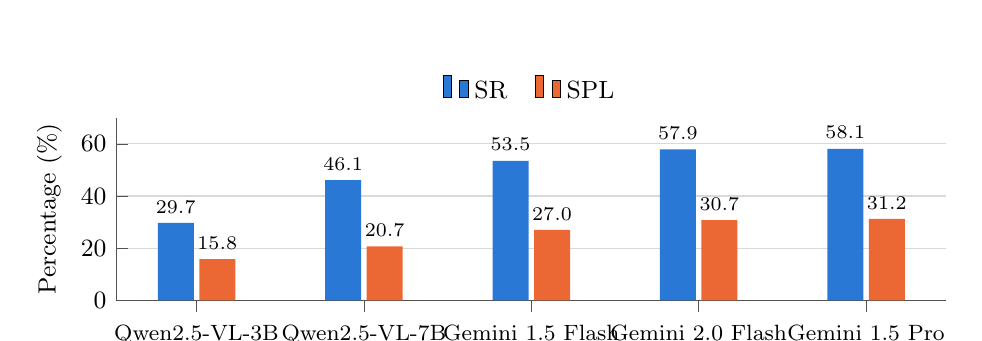
\begin{tikzpicture}
\begin{axis}[
  ybar=2pt, bar width=13pt, width=\textwidth, height=3.9cm,
  symbolic x coords={Qwen2.5-VL-3B,Qwen2.5-VL-7B,Gemini 1.5 Flash,Gemini 2.0 Flash,Gemini 1.5 Pro},
  xtick=data, enlarge x limits=0.12, ymin=0, ymax=70,
  ylabel={Percentage (\%)}, ylabel style={font=\small},
  ymajorgrids, grid style={gridgray}, axis line style={inkgray}, tick style={inkgray},
  axis x line*=bottom, axis y line*=left, tick label style={font=\small}, x tick label style={font=\footnotesize},
  nodes near coords, nodes near coords style={font=\scriptsize, text=black},
  every node near coord/.append style={/pgf/number format/fixed, /pgf/number format/fixed zerofill, /pgf/number format/precision=1},
  legend style={at={(0.5,1.02)}, anchor=south, legend columns=-1, draw=none, font=\small, /tikz/every even column/.append style={column sep=8pt}},
]
\addplot[fill=seriesA, draw=none] coordinates {(Qwen2.5-VL-3B,29.7) (Qwen2.5-VL-7B,46.1) (Gemini 1.5 Flash,53.5) (Gemini 2.0 Flash,57.9) (Gemini 1.5 Pro,58.1)};
\addplot[fill=seriesB, draw=none] coordinates {(Qwen2.5-VL-3B,15.8) (Qwen2.5-VL-7B,20.7) (Gemini 1.5 Flash,27.0) (Gemini 2.0 Flash,30.7) (Gemini 1.5 Pro,31.2)};
\legend{SR, SPL}
\end{axis}
\end{tikzpicture}
\caption{WMNav performance on HM3D v0.1 with different VLMs, plotted from \cite{p4}}
\label{fig:wmnav_chart}
\end{figure}

\subsection{Discussion}

\paragraph{}
WMNav shows that pre-trained VLMs can act as abstract world models: prediction replaces costly exploration and curiosity scoring enforces reliable outputs. However, it relies on repeated calls to large, often proprietary VLMs and has been tested only in simulation.

% ================= CHAPTER 4: DISCUSSION & COMPARISON =================
\chapter{Discussion \& Comparison}

\paragraph{}
This chapter presents a detailed comparative analysis of the four reviewed research papers that instantiate world models across the manipulation, locomotion, and navigation domains of embodied AI. These studies collectively demonstrate how predictive internal models---whether explicit physics simulations, motion-augmented Gaussian fields, latent recurrent dynamics, or VLM-based imagination---are transforming robotics from reactive perception--action mappings into anticipatory, plan-before-act intelligence. While each paper shares the common goal of predicting the future state of the world to improve decision-making, they differ fundamentally in representation, learning signals, planning mechanisms, and deployment platforms. The following sections critically evaluate their contributions, advantages, and limitations, offering insights into their comparative strengths and areas for further improvement.

\section{Analytical Focus}

\paragraph{} Each paper addresses a distinct challenge in world-model-driven embodied AI. Paper \cite{p1} tackles \textbf{precise, goal-conditioned manipulation of unseen articulated objects}, turning perception into search inside a physics simulator via an explicit digital twin. Paper \cite{p2} addresses the \textbf{mismatch between static scene understanding and dynamic action generation} by embedding motion into an explicit Gaussian scene representation, so actions are read directly from predicted geometry. Paper \cite{p3} targets \textbf{perception under partial observability} in legged locomotion, compressing depth-image and proprioceptive histories into a latent state that replaces hand-designed privileged information. Paper \cite{p4} explores \textbf{prediction without any environment-specific training}, delegating world modeling to pre-trained VLMs' commonsense knowledge for zero-shot navigation.
Together, these studies span physics-grounded, geometry-grounded, latent, and semantic designs, united by imagining outcomes before acting.

\section{Comparison of Methodologies}

\paragraph{} Table~\ref{tab:wm_comparison} summarizes the methodology, advantages, and limitations of each work. The table highlights that the four systems occupy complementary positions: none dominates on every axis, and each limitation is, to a large extent, the mirror image of the corresponding advantage.

{\renewcommand{\arraystretch}{1.45}
\setlength{\tabcolsep}{6pt}
\small
\begin{longtable}{|p{3.3cm}|p{3.55cm}|p{3.55cm}|p{3.55cm}|}
\caption{Comparison of world-model approaches for embodied AI}\label{tab:wm_comparison}\\
\hline
\textbf{Paper} & \textbf{Methodology} & \textbf{Advantages} & \textbf{Limitations} \\
\hline
\endfirsthead
\hline
\textbf{Paper} & \textbf{Methodology} & \textbf{Advantages} & \textbf{Limitations} \\
\hline
\endhead
\hline
\endfoot
\hline
\endlastfoot
DexSim2Real$^2$ \cite{p1}: Explicit world model for articulated object dexterous manipulation
 &
Interactive perception + 3D AIGC digital twin construction; sampling-based MPC (iCEM) with eigengrasp dimensionality reduction for dexterous hands. &
Demonstration-free and RL-free; high precision (avg.\ error $\approx 7^{\circ}$); supports multiple end effectors and unseen strategies such as tool use. &
Requires observable state changes during interaction; 3D AIGC meshes may misalign for novel objects; minutes-scale trajectory search. \\
\hline
GAF \cite{p2}: Gaussian Action Field as a 4D representation for dynamic world modeling &
Extends 3DGS with learnable per-Gaussian motion; ViT-based feed-forward reconstruction; ICP-derived init action refined by action-vision-aligned diffusion. &
Unifies reconstruction, prediction, and action; needs only sparse unposed RGB; +7.3\% success over the best baseline and real-time inference ($<$0.3 s). &
Lacks semantic/task-level understanding; partial occlusions cause misaligned contacts; needs some real action data for refinement. \\
\hline
WMP \cite{p3}: World Model-based Perception for visual legged locomotion &
RSSM world model trained in simulation; policy on recurrent latent state via asymmetric actor--critic PPO; AMP-style natural-gait rewards. &
Removes privileged teacher--student gap; near-teacher returns; best real-world traversal on Unitree A1 (Gap 85 cm, Climb 55 cm, Crawl 22 cm). &
World model bounded by simulator fidelity; latency forces coarse model interval ($k=5$); no real-data model training yet. \\
\hline
WMNav \cite{p4}: Integrating Vision-Language Models into world models for object goal navigation &
PredictVLM scores directions into an online Curiosity Value Map; subtask decomposition; two-stage action proposer; all reasoning by prompted VLMs. &
Zero-shot and training-free; +3.2\%/+13.5\% SR over the best zero-shot methods on HM3D/MP3D; reduces risky exploration through prediction. &
Dependent on proprietary VLM capability and cost; susceptible to hallucination; indoor object-goal setting only. \\
\end{longtable}}

\section{Representation, Learning Signal, and Control Strategy}

\paragraph{} A finer-grained comparison of how each world model is represented, built, and used is given in Table~\ref{tab:repr}. Two observations stand out. First, the \emph{construction cost} of the world model is inversely related to its \emph{generality}: DexSim2Real$^2$ builds a new, highly accurate model for every object instance; GAF and WMP learn a model per task family; and WMNav uses a single frozen model for every environment and category. Second, the \emph{control strategy} follows from the representation: an explicit simulator invites search (MPC), a geometric field invites registration (ICP) followed by learned refinement, a latent state invites a learned policy, and a semantic model invites prompting.

{\renewcommand{\arraystretch}{1.35}
\begin{table}[htbp]
\centering
\caption{World-model representation, construction, and use in the four reviewed works}\label{tab:repr}
\footnotesize
\begin{tabularx}{\textwidth}{|p{2.35cm}|X|X|X|X|}
\hline
\textbf{Aspect} & \textbf{DexSim2Real$^2$} & \textbf{GAF} & \textbf{WMP} & \textbf{WMNav} \\ \hline
World state & URDF digital twin (meshes + joints) & 3D Gaussians $\{\mu,f\}$ & RSSM state $(h_t,z_t)$ & Curiosity Value Map + subtask cost \\ \hline
Transition model & Physics engine (SAPIEN) & Learned displacement $\Delta\mu$ & GRU recurrent model & VLM imagination (PredictVLM) \\ \hline
How it is obtained & $K$ interactions + 3D AIGC + kinematic estimation & Trained on RGB video frames & Trained on simulated rollouts & Pre-trained VLM, prompted \\ \hline
Supervision & None for the model itself; affordance from sim or human video & Photometric (LPIPS + MSE); 20 demos/task for refinement & Reconstruction + KL; PPO rewards & None (training-free) \\ \hline
Decision making & iCEM sampling-based MPC & ICP init action + diffusion refinement & PPO policy on $\mathrm{sg}(h_t)$ & PlanVLM + ReasonVLM with action proposer \\ \hline
Action space & Joint increments (7--9 D with eigengrasp) & End-effector poses + gripper state & 12 joint targets at 50 Hz & Polar vectors $(r,\theta)$ \\ \hline
Decision latency & 1.5--3 min per trajectory & $<$0.3 s per 8 actions & Real time on Jetson NX & Several VLM calls per step \\ \hline
\end{tabularx}
\end{table}}

\section{Model Performance and Evaluation}

\paragraph{} All four studies provide rigorous quantitative evaluation on real robots or standard benchmarks.
\begin{itemize}
  \item Paper \cite{p1} achieved average manipulation errors of $7.2^{\circ}$ (laptop) and $6.8^{\circ}$ (cabinet) with the suction gripper versus $16.0^{\circ}$/$15.3^{\circ}$ for UMPNet, and world-model construction accuracy with joint-axis angle error below $9^{\circ}$ across four object categories.
  \item Paper \cite{p2} reported a 60.4\% average success rate on nine RLBench tasks, exceeding Diffusion Policy by 15.7\%, Act3D by 7.3\%, and ManiGaussian by 10.3\%, alongside +11.54 dB PSNR reconstruction gains and 6--10/10 success on five real Franka tasks.
  \item Paper \cite{p3} attained near-teacher returns in simulation and the best real-world traversal performance reported on a Unitree A1: Gap 85 cm, Climb 55 cm, Tilt 28 cm, and Crawl 22 cm, terrains on which the privileged student baseline partially or completely fails.
  \item Paper \cite{p4} delivered state-of-the-art zero-shot navigation with 58.1\% SR / 31.2\% SPL on HM3D and 45.4\% SR / 17.2\% SPL on MP3D, and 72.2\% SR on HM3D v0.2 in ablation configuration.
\end{itemize}
Despite these strong results, the evaluation settings differ substantially---single fixed-arm tabletop scenes, RLBench and Franka tasks, indoor quadruped courses, and Habitat photorealistic scans---so cross-paper numbers indicate domain-specific maturity rather than direct superiority of one representation over another. Table~\ref{tab:platforms} summarizes the experimental platforms.

{\renewcommand{\arraystretch}{1.35}
\begin{table}[htbp]
\centering
\caption{Experimental platforms and evaluation protocols}\label{tab:platforms}
\footnotesize
\begin{tabularx}{\textwidth}{|p{2.35cm}|X|X|X|X|}
\hline
\textbf{Aspect} & \textbf{DexSim2Real$^2$} & \textbf{GAF} & \textbf{WMP} & \textbf{WMNav} \\ \hline
Robot & ROKAE xMate3Pro 7-DOF arm & Franka Emika Panda & Unitree A1 quadruped & Simulated cylindrical agent \\ \hline
End effector / body & Suction, Robotiq 2F-140, Allegro Hand, XHand & Panda Hand & 12 actuated joints & Radius 0.18 m, height 0.88 m \\ \hline
Sensors & RealSense D415 + side RGB camera & 3 RealSense D435i (2 fixed, 1 wrist) & Front RealSense D435i depth + proprioception & RGB-D $640\times480$, HFoV $79^{\circ}$ \\ \hline
Simulator & SAPIEN & RLBench (CoppeliaSim) & Isaac Gym (\texttt{legged\_gym}) & Habitat \\ \hline
Benchmarks / objects & Drawers, cabinets, laptops, lamps & 9 RLBench tasks + 5 real tasks & 6 terrains, 5 real terrains & HM3D v0.1/v0.2, MP3D \\ \hline
Main metrics & $|\delta|$, $|\delta_r|$, RDE, IoU, axis error & Success rate, PSNR, SSIM, LPIPS & Return, tracking error, success rate & SR, SPL \\ \hline
\end{tabularx}
\end{table}}

\section{Data and Environment Utilization}

\paragraph{} Data requirements diverge sharply across the four systems. Paper \cite{p1} needs only $K+1$ real observation frames per object plus offline affordance training data, sourced either from simulated interaction (Where2Act on SAPIEN assets) or from large-scale egocentric human videos (VRB), the latter removing dependence on scarce interactable 3D assets. Paper \cite{p2} trains from RGB video frames alone for reconstruction---no depth, poses, or 3D ground truth---plus 20 demonstrations per RLBench task for action refinement. Paper \cite{p3} exploits massively parallel simulation (4096 robots in Isaac Gym) with terrain curriculum and domain randomization, requiring no real-world data at all. Paper \cite{p4} requires no training data whatsoever, relying entirely on frozen VLMs and the HM3D/MP3D evaluation scenes. This progression---from instance-specific reconstruction to zero-data prediction---highlights how world models can trade data collection against prior knowledge, whether physical, geometric, or semantic.

\section{Scalability and Deployment Potential}

\paragraph{} Deployment characteristics vary significantly across the proposed systems:
\begin{itemize}
  \item Paper \cite{p1}'s pipeline runs trajectory search in about 1.5--3 minutes per task on a desktop CPU/GPU, suitable for deliberate household manipulation but not for reactive control; its modular design extends naturally to new end effectors and tools.
  \item Paper \cite{p2} operates feed-forward on a single GPU with sub-0.3 s action prediction and parallel prediction--execution threads, making it genuinely real-time and deployable on real manipulators.
  \item Paper \cite{p3} runs fully on-board a Jetson NX without external computation, with the model interval $k=5$ chosen explicitly to absorb 40 ms of sensing and inference latency---evidence of careful hardware--algorithm co-design.
  \item Paper \cite{p4}'s reliance on cloud VLM APIs introduces latency and cost per step, restricting current deployment to non-time-critical navigation, though the framework improves automatically as VLMs advance.
\end{itemize}
In real-world implementation, the trade-off between model fidelity, planning latency, and computational footprint must be balanced against task tempo: manipulation tolerates minutes of deliberation, locomotion demands 50 Hz reactivity, and navigation lies in between.

\section{Interpretability and Trustworthiness}

\paragraph{} World models differ markedly in how inspectable their predictions are. Paper \cite{p1} is the most interpretable: its digital twin is a human-readable URDF with explicit joint types, axes, and meshes, and planned trajectories can be visualized in simulation before execution. Paper \cite{p2} renders photorealistic images of both current and predicted future scenes, allowing direct visual verification of what the model believes will happen. Paper \cite{p4} produces natural-language explanations for every directional score and subtask, and its feedback loop between plan and observation explicitly counteracts VLM hallucination. Paper \cite{p3}, by contrast, encodes knowledge in a latent state; interpretability is indirect, through decoded depth predictions and t-SNE terrain clustering. This ordering suggests a tension between representation compactness and transparency that future world-model designs must negotiate.

\section{A Design-Space View}

\paragraph{} The comparison can be condensed into a two-dimensional design space (Figure~\ref{fig:design_space}). The vertical axis represents \emph{physical and geometric fidelity}---how precisely the model captures shapes, contacts, and dynamics---while the horizontal axis represents \emph{semantic breadth and generality}---how many objects, categories, and environments the same model covers without retraining. DexSim2Real$^2$ sits at the high-fidelity, instance-specific corner; GAF trades a little physical grounding for a learned, task-family-level model; WMP captures terrain dynamics compactly but only for the terrain distribution it was trained on; and WMNav reaches the broadest semantic coverage with essentially no physical modelling. The empty upper-right region---models that are both physically precise and semantically general---is where future hybrid world models are expected to lie.

\begin{figure}[htbp]
\centering
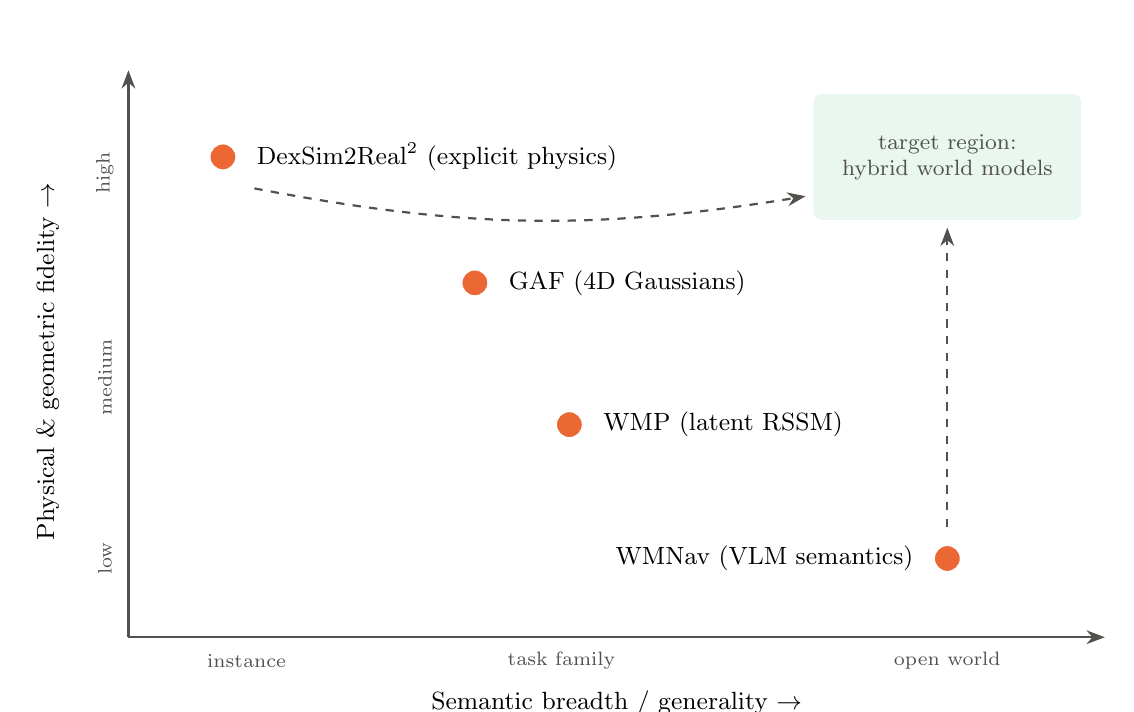
\begin{tikzpicture}[>=Stealth, thick]
\fill[boxgreen!70, rounded corners=3pt] (8.7,5.3) rectangle (12.1,6.9);
\node[font=\footnotesize, align=center, text=inkgray] at (10.4,6.1) {target region:\\hybrid world models};
\draw[->, inkgray] (0,0) -- (12.4,0);
\draw[->, inkgray] (0,0) -- (0,7.2);
\node[font=\small, anchor=north] at (6.2,-0.55) {Semantic breadth / generality $\rightarrow$};
\node[font=\small, anchor=south, rotate=90] at (-0.75,3.5) {Physical \& geometric fidelity $\rightarrow$};
\foreach \x/\l in {1.5/instance, 5.5/task family, 10.4/open world} \node[font=\scriptsize, text=inkgray] at (\x,-0.3) {\l};
\foreach \y/\l in {1/low, 3.3/medium, 5.9/high} \node[font=\scriptsize, text=inkgray, rotate=90] at (-0.3,\y) {\l};
\filldraw[fill=seriesB, draw=white, line width=1pt] (1.2,6.1) circle (5pt);
\node[font=\small, anchor=west] at (1.5,6.1) {DexSim2Real$^2$ (explicit physics)};
\filldraw[fill=seriesB, draw=white, line width=1pt] (4.4,4.5) circle (5pt);
\node[font=\small, anchor=west] at (4.7,4.5) {GAF (4D Gaussians)};
\filldraw[fill=seriesB, draw=white, line width=1pt] (5.6,2.7) circle (5pt);
\node[font=\small, anchor=west] at (5.9,2.7) {WMP (latent RSSM)};
\filldraw[fill=seriesB, draw=white, line width=1pt] (10.4,1.0) circle (5pt);
\node[font=\small, anchor=east] at (10.1,1.0) {WMNav (VLM semantics)};
\draw[->, dashed, inkgray] (1.6,5.7) to[bend right=10] (8.6,5.6);
\draw[->, dashed, inkgray] (10.4,1.4) -- (10.4,5.2);
\end{tikzpicture}
\caption{Qualitative placement of the reviewed world models in a fidelity--generality design space. Positions are a qualitative synthesis of the comparison in this chapter, not measured quantities.}
\label{fig:design_space}
\end{figure}

\section{Innovation and Research Contributions}

\paragraph{} Each paper introduces novel elements that advance the state-of-the-art:
\begin{itemize}
  \item \textbf{Paper \cite{p1}} --- Combines interactive perception, 3D AIGC digital-twin reconstruction of multi-part articulated objects, and eigengrasp-reduced sampling-based MPC for dexterous hands, with video-based affordance learning replacing scarce simulation assets.
  \item \textbf{Paper \cite{p2}} --- Introduced the V-4D-A paradigm and the Gaussian Action Field, extracting actions from predicted Gaussian motion via ICP and refining them with actionable multiview RGB guidance.
  \item \textbf{Paper \cite{p3}} --- First application of Dreamer-style RSSM world modeling to challenging vision-based legged locomotion with successful sim-to-real transfer, replacing the privileged learning paradigm.
  \item \textbf{Paper \cite{p4}} --- Proposed a fully modular VLM world model for ZSON, with the online Curiosity Value Map as quantitative predictive memory and hallucination-mitigating subtask feedback.
\end{itemize}
Together, these contributions indicate a shift toward embodied agents that construct, maintain, and exploit predictive models of their surroundings as a first-class component of the control loop.

\section{Practical Relevance and Real-World Application}

\paragraph{} From a deployment perspective, Paper \cite{p1} targets assistive and household robotics where precise operation of cabinets, drawers, laptops, and lamps matters, and its tool-use extension previews service robots that improvise with available implements. Paper \cite{p2}'s real-time pipeline suits industrial and tabletop manipulation cells where sparse cameras are cheaper than calibrated depth rigs. Paper \cite{p3} directly advances inspection, delivery, and search-and-rescue quadrupeds that must negotiate stairs, gaps, and crawl spaces outdoors, as demonstrated in park deployments. Paper \cite{p4} addresses domestic assistance---finding objects in unseen homes---without any environment-specific setup. Collectively, these models cover deliberate manipulation, agile locomotion, and semantic navigation, demonstrating the versatility of the world-model paradigm across the full spectrum of embodied robotics.

\section{Overall Comparative Insights}

\paragraph{} In synthesis, Paper \cite{p1} prioritizes precision through explicit physics, Paper \cite{p2} unification of prediction and action through 4D geometry, Paper \cite{p3} perceptual compression through latent dynamics, and Paper \cite{p4} zero-shot semantics through foundation models. Each contributes to a different dimension of world-model development:
\begin{itemize}
  \item \textbf{Precision and Physical Grounding:} Papers \cite{p1}--\cite{p2} anchor predictions in explicit geometry and physics, enabling accurate contact-rich manipulation.
  \item \textbf{Sample Efficiency:} Papers \cite{p1} and \cite{p3} show that physics priors and simulated world-model training dramatically cut real-world data needs.
  \item \textbf{Real-Time Capability:} Papers \cite{p2}--\cite{p3} achieve on-board, low-latency inference; Paper \cite{p1} trades latency for precision; Paper \cite{p4} is bounded by VLM API speed.
  \item \textbf{Generality and Zero-Shot Ability:} Paper \cite{p4} generalizes to unseen scenes and categories without training, while Paper \cite{p1} generalizes to unseen actions such as tool use.
\end{itemize}

\paragraph{}
In conclusion, the four reviewed research papers collectively mark a significant evolution in embodied AI. The fusion of explicit digital twins, dynamic Gaussian representations, latent recurrent dynamics, and VLM-based imagination has transformed robots from reactive controllers into agents capable of predicting, planning, and explaining their behavior. Future research will likely converge these paradigms---combining the precision of explicit models, the real-time efficiency of feed-forward 4D representations, the compression of latent states, and the semantic breadth of foundation models---to create unified, resilient world models for the next generation of embodied intelligent systems.

% ================= CHAPTER 5: APPLICATIONS =================
\chapter{Applications}

\paragraph{} World-model-driven embodied agents are moving from laboratory demonstrations toward practical use. This chapter surveys application areas in which the capabilities demonstrated by the reviewed works---precise articulated manipulation, dynamic scene prediction, agile perceptive locomotion, and semantic navigation---are directly relevant. The discussion is grounded in the demonstrations reported by the papers and indicates which family of world model is most suitable for each setting.

\section{Household and Assistive Robotics}

\paragraph{} Homes are full of articulated objects: kitchen cabinets, refrigerators, drawers, ovens, microwaves, laptops, and lamps. An assistive robot that helps elderly or physically impaired people must open and close these objects to specific configurations---a refrigerator door just wide enough to reach inside, a drawer opened half-way---rather than simply ``open'' or ``closed''. DexSim2Real$^2$ addresses exactly this goal-conditioned setting and demonstrates it on drawers, cabinets, laptops, lamps, and a multi-part refrigerator. Its ability to build a model after a single interaction is important in homes, where every object instance is different and collecting demonstrations for each is infeasible. The tool-use capability further suggests robots that can reach an object at the back of a counter with a utensil, or pull a small drawer with a hook.

\section{Industrial and Warehouse Manipulation}

\paragraph{} In factories and fulfilment centres, robots must handle varied parts, operate fixtures, and recover from disturbances in real time. GAF's feed-forward pipeline, which infers actions from two unposed RGB views in under 0.3 s and generalizes across the workspace, suits such manipulation cells, where installing and calibrating dense depth sensors is costly. The ability to render predicted future scenes also supports monitoring: a supervisor or an automated checker can compare the predicted outcome of an action with what actually happens and flag anomalies. Digital twins of the kind built by DexSim2Real$^2$ are likewise valuable for offline programming and virtual commissioning, in which robot motions are planned and verified in simulation before being deployed to the production line.

\section{Inspection, Search-and-Rescue, and Field Robotics}

\paragraph{} Legged robots are increasingly deployed for industrial inspection (power plants, oil and gas facilities, construction sites), public safety, and search-and-rescue in collapsed or cluttered environments. These settings feature gaps, steps, narrow passages, and overhanging obstacles---exactly the Gap, Climb, Tilt, and Crawl terrains of WMP. Because WMP runs entirely on the robot's onboard computer and does not require hand-designed privileged information for each obstacle type, it is well matched to field deployment where communication may be unreliable and obstacles are not known in advance. The park experiments, in which the robot climbed stairs, mounted platforms up to 45 cm, and walked on grass and gravel, illustrate this potential.

\section{Domestic Service and Semantic Navigation}

\paragraph{} A service robot asked to ``bring the remote from the sofa'' or ``check whether the stove is off'' must first find the relevant object in a home it may never have mapped. Zero-shot object navigation, as addressed by WMNav, is a key capability for such robots. Because WMNav needs no training on the target environment and no pre-built maps, it could be deployed in a new home immediately, using commonsense priors (sofas are in living rooms, beds in bedrooms) to search efficiently. Similar reasoning applies to hospitality and retail robots that must locate items or locations in large indoor spaces, and to mobile manipulators that combine navigation with the manipulation capabilities of the other reviewed works.

\section{Healthcare and Laboratory Automation}

\paragraph{} Hospitals and laboratories contain many articulated devices---sample cabinets, instrument doors, drawers---and require precise, safe, and verifiable operation. Explicit world models are attractive here because every planned motion can be simulated and inspected before execution, providing a natural point for safety checks. Predictive models also help robots operate around people: by anticipating how a scene will evolve, a robot can avoid actions whose predicted outcome is unsafe.

\section{Simulation, Testing, and Education}

\paragraph{} Beyond deployment, world models serve as tools for robot development. Digital twins reconstructed from a few observations can populate simulation environments with realistic articulated assets, alleviating the shortage of interactable 3D models noted by the DexSim2Real$^2$ authors. Latent world models that predict real-world observations, as in WMP, can be used to test policies offline before hardware trials. VLM-based world models can generate high-level plans and explanations that make robot behaviour easier to understand for students and non-expert users.

{\renewcommand{\arraystretch}{1.35}
\begin{table}[htbp]
\centering
\caption{Application domains and the most suitable world-model families}\label{tab:applications}
\small
\begin{tabularx}{\textwidth}{|p{3.6cm}|X|p{3.2cm}|}
\hline
\textbf{Application domain} & \textbf{Key requirement} & \textbf{Most relevant work} \\ \hline
Household / assistive manipulation & Precise, goal-conditioned operation of unseen articulated objects & DexSim2Real$^2$ \cite{p1} \\ \hline
Industrial manipulation cells & Real-time action inference from sparse, cheap cameras & GAF \cite{p2} \\ \hline
Inspection and search-and-rescue & On-board perceptive locomotion over unknown obstacles & WMP \cite{p3} \\ \hline
Domestic service navigation & Zero-shot search for objects in unmapped homes & WMNav \cite{p4} \\ \hline
Healthcare / laboratory automation & Verifiable, inspectable plans before execution & DexSim2Real$^2$ \cite{p1}, GAF \cite{p2} \\ \hline
Simulation and testing & Realistic assets and offline policy evaluation & DexSim2Real$^2$ \cite{p1}, WMP \cite{p3} \\ \hline
\end{tabularx}
\end{table}}

% ================= CHAPTER 6: CHALLENGES AND FUTURE DIRECTIONS =================
\chapter{Challenges and Future Directions}

\paragraph{}
Despite significant progress in world-model-driven embodied AI, several technical, operational, and practical barriers still hinder effective deployment in unstructured real-world environments. This chapter first summarizes the challenges identified in each of the four reviewed studies, then discusses cross-cutting challenges common to all world models, and finally outlines promising research directions.

\section{Challenges Identified in the Reviewed Works}

\subsection{DexSim2Real$^2$: Explicit World Model for Dexterous Manipulation}

\paragraph{} The framework infers kinematic structure by analyzing inter-frame differences, so it strictly requires observable state changes of every movable part during interactive perception; parts that cannot be moved or seen cannot be modeled. For novel or uncommon objects, existing 3D AIGC techniques may generate meshes that are imperfectly aligned with real-world observations, degrading digital-twin accuracy and hence manipulation precision, since manipulation error correlates positively with joint position and orientation errors of the model. Real objects also exhibit unmodeled dynamics---elastic deformation of laptop lids and rail gaps that turn ideal prismatic joints into multi-DOF joints---which the rigid simulation cannot capture. Finally, trajectory search takes 1.5--3 minutes per task, precluding reactive behavior, and the current system is limited to a single object manipulated by one fixed arm.

\subsection{GAF: 4D Gaussian World Modeling}

\paragraph{} Although GAF unifies reconstruction, prediction, and action, its purely geometric world model lacks semantic and task-level understanding, limiting context-aware manipulation. Reconstruction errors under partial occlusion lead to misaligned contacts during interaction; without the diffusion-based refinement stage, executed init actions frequently fail, showing that visually plausible motion is not automatically physically feasible. The refinement stage reintroduces a dependence on real action demonstrations, and real-world failures concentrated in grasping (apple, door handle) reveal the absence of force feedback, suggesting the need for tactile sensing and richer gripper-state training data. Multi-task training also reduces performance on dissimilar tasks such as \emph{lift lid up}.

\subsection{WMP: World Model-based Perception for Locomotion}

\paragraph{} Because the RSSM is trained exclusively on simulated data, it cannot exceed the simulator's fidelity; unmodeled real-world dynamics and never-seen obstacle shapes manifest as prediction discrepancies (e.g., the Crawl obstacle's shape differs in predicted depth images). Real-world latency of depth acquisition and on-board inference ($\approx$40 ms) forces a coarser world-model interval ($k=5$), sacrificing the higher returns that faster model updates achieve in simulation. Backpropagating gradients through long RSSM training segments is inefficient, restricting usable history length to seconds. Training the world model with mixed simulated and real data, and incorporating additional sensing modalities such as touch, remain open future work.

\subsection{WMNav: VLM World Models for Navigation}

\paragraph{} The framework inherits the weaknesses of its foundation models: VLM hallucination can inject erroneous predictions into the Curiosity Value Map, and although subtask feedback and quantitative scoring mitigate this, they cannot eliminate it. Performance scales strongly with VLM capability---the best open-source model tested, Qwen2.5-VL-7B (46.1\% SR), trails Gemini 1.5 Pro (58.1\% SR) by 12 points---creating cost, latency, and accessibility dependencies on commercial APIs. Each navigation step requires multiple VLM calls, limiting real-time operation. The evaluation is confined to indoor object-goal tasks in Habitat scenes; extension to real robots, dynamic environments, outdoor settings, and instruction-following tasks is untested.

\section{Cross-Cutting Challenges}

\paragraph{} \textbf{Model fidelity and compounding error.} Every world model is an approximation, and errors compound when a model is rolled forward over long horizons. Planners and policies can exploit model errors, choosing actions that look good in the model but fail in reality. DexSim2Real$^2$ shows that manipulation error grows with modelling error, and GAF shows that visually plausible predictions may not be physically feasible. Quantifying and propagating model uncertainty, and re-planning frequently with fresh observations, are essential mitigations.

\paragraph{} \textbf{The sim-to-real gap.} Explicit and latent world models built or trained in simulation inherit the simulator's simplifications: rigid bodies, idealized joints, simplified contacts, and clean sensing. Domain randomization, latency modelling, and real-to-sim reconstruction reduce but do not remove this gap, and deformable, granular, or fluid materials remain especially difficult.

\paragraph{} \textbf{Computation and latency.} There is a persistent tension between model richness and decision speed. Sampling-based MPC over a physics engine takes minutes, VLM calls take seconds, and on-board locomotion must run at tens of hertz on embedded hardware. Selecting the right model for the task tempo, and distilling slow models into fast policies, is an open engineering problem.

\paragraph{} \textbf{Semantic grounding versus physical grounding.} Geometric and physical world models understand shape and dynamics but not meaning; semantic world models understand meaning but not precise geometry or physics. Tasks such as ``open the drawer that contains the scissors'' require both, and no reviewed system provides both.

\paragraph{} \textbf{Reliability and hallucination of foundation models.} As foundation models are increasingly used inside the control loop, their tendency to produce confident but wrong outputs becomes a safety concern. Structured outputs, quantitative scoring, cross-checking against observations, and geometric verification (as in WMNav's distance-based stopping) are necessary safeguards.

\paragraph{} \textbf{Evaluation and benchmarking.} The reviewed works use different robots, simulators, tasks, and metrics, making direct comparison impossible. Standardized benchmarks that evaluate world models across manipulation, locomotion, and navigation---including prediction quality, downstream task success, and computational cost---would accelerate progress.

\section{Future Research Directions}

\paragraph{} Building on the limitations above and on the future work proposed by the authors of the reviewed papers, several promising directions emerge:
\begin{itemize}
  \item \textbf{Hybrid geometric--semantic world models:} enriching explicit and Gaussian world models with semantic priors from foundation models, so that a single representation supports both precise contact reasoning and language-level goals; GAF's authors explicitly propose adding language modelling.
  \item \textbf{Mixed simulated and real training:} training latent world models on a mixture of simulated and real-world experience to reduce the sim-to-real gap, as suggested for WMP, and continually updating the model during deployment.
  \item \textbf{Multi-modal sensing:} incorporating tactile, force, and audio signals into world models to capture contact events and material properties that vision cannot observe, addressing failure modes observed in GAF and proposed for WMP.
  \item \textbf{Scene-level digital twins and mobile manipulation:} scaling from single-object twins to complete rooms and houses for long-horizon mobile manipulation, as proposed by the DexSim2Real$^2$ authors, and combining such twins with semantic navigation of the WMNav type.
  \item \textbf{Learning rewards from videos and language:} replacing hand-designed dense rewards with rewards generated from human videos or natural-language descriptions, reducing the engineering effort of MPC-based systems.
  \item \textbf{Efficient inference and distillation:} distilling slow planners and large VLMs into compact policies or smaller on-device models, enabling world-model reasoning at control rates on embedded hardware.
  \item \textbf{Uncertainty-aware and safe planning:} equipping world models with calibrated uncertainty so that planners can avoid regions where the model is unreliable and actively gather information when uncertainty is high, extending the interactive perception idea of DexSim2Real$^2$.
  \item \textbf{Unified benchmarks:} developing shared evaluation suites that measure world-model prediction accuracy and downstream embodied performance across domains.
\end{itemize}

\section{Ethical and Societal Considerations}

\paragraph{} As world-model-driven robots move into homes, hospitals, and public spaces, their technical capabilities must be matched by attention to their wider impact. \textbf{Safety} is the foremost concern: a robot that plans inside an imperfect model can act confidently on wrong predictions, so safety constraints, conservative fall-back behaviours, and human oversight remain necessary even when the model is usually accurate. \textbf{Privacy} is a second concern: systems such as DexSim2Real$^2$ and WMNav continuously capture images of the private spaces in which they operate, and navigation agents that send panoramic views of a home to cloud-hosted VLMs raise questions about where that data is stored and who can access it. On-device models and data-minimizing designs are therefore desirable.

\paragraph{} \textbf{Accountability and transparency} matter when a robot causes damage or fails at a task. World models that can be rendered or queried---digital twins, Gaussian renderings, and natural-language explanations---make it easier to reconstruct why a decision was taken, which supports debugging, certification, and user trust. Finally, \textbf{accessibility and sustainability} deserve attention: dependence on large proprietary models and powerful GPUs increases cost and energy consumption and may concentrate capability in a few organizations, whereas open, efficient models broaden access for researchers, students, and small companies.

\section{Summary}

\paragraph{}
In summary, world-model-based embodied AI faces challenges in model fidelity, sim-to-real alignment, semantic grounding, latency, and dependence on foundation-model quality. Addressing these issues requires hybrid training on simulated and real data, integration of tactile and force sensing, semantic priors within geometric world models, hallucination-resistant prompting and verification mechanisms, and efficient on-board inference. Progress along these directions will be essential to develop reliable, transparent, and broadly deployable world models for next-generation embodied intelligent systems.

% ================= CHAPTER 7: CONCLUSION =================
\chapter{Conclusion}

\paragraph{}
The integration of \textbf{world models} into \textbf{embodied AI} marks a major milestone in the evolution of intelligent robotics. Purely reactive policies, which map current observations directly to actions, often fail under the partial observability, complex dynamics, and open-endedness of the physical world. World-model-driven agents overcome these limitations by maintaining an internal, predictive representation of their environment---imagining the consequences of candidate actions before execution---thereby enabling precise planning, efficient exploration, and robust sim-to-real transfer across manipulation, locomotion, and navigation.

\paragraph{}
This study reviewed four key research contributions illustrating the diverse realizations of world models in embodied AI.
\textbf{Paper \cite{p1}} (DexSim2Real$^2$) constructed an \textit{explicit} digital-twin world model of unseen articulated objects through interactive perception and 3D AIGC reconstruction, enabling sampling-based MPC with eigengrasp-reduced dexterous hands to achieve goal-conditioned manipulation errors of only a few degrees---without demonstrations or reinforcement learning---and generalizing to advanced skills such as tool use.
\textbf{Paper \cite{p2}} (GAF) introduced a 4D Gaussian Action Field that unifies scene reconstruction, future prediction, and action extraction in a single feed-forward framework, improving average manipulation success by 7.3\% over state-of-the-art baselines while running in real time from sparse unposed RGB views.
\textbf{Paper \cite{p3}} (WMP) demonstrated that an RSSM world model trained entirely in simulation can serve as the perceptual backbone for visual legged locomotion, achieving the best reported traversal performance on a Unitree A1 quadruped and eliminating the teacher--student gap of privileged learning.
Finally, \textbf{Paper \cite{p4}} (WMNav) integrated Vision-Language Models into a modular world model with an online Curiosity Value Map, attaining state-of-the-art zero-shot object goal navigation on HM3D and MP3D without any task-specific training.

\paragraph{}
Taken together, these works trace a coherent design space---explicit physics-based, geometry-embedded, latent, and semantic world models---each optimizing a different balance among precision, data efficiency, latency, interpretability, and generality. The comparative analysis indicates that no single representation dominates; rather, the appropriate world model depends on the tempo and structure of the task at hand. The key lessons of this seminar can be summarized as follows:
\begin{itemize}
  \item \textbf{Predicting before acting works across domains:} the same principle improves precision in manipulation, robustness in locomotion, and efficiency in navigation.
  \item \textbf{Priors substitute for data:} physics engines, 3D geometry, simulated experience, and internet-scale pre-training each reduce the amount of task-specific real-world data required.
  \item \textbf{Representation determines control strategy:} explicit simulators favour search, geometric fields favour registration and refinement, latent states favour learned policies, and semantic models favour prompting.
  \item \textbf{Interpretability is a practical asset:} renderable and inspectable models make it possible to verify plans before execution, an important property for safe deployment.
\end{itemize}

\paragraph{}
Future research is expected to converge these paradigms: enriching explicit and Gaussian world models with semantic priors from foundation models, training latent models on mixtures of simulated and real experience, incorporating tactile and force sensing, and scaling from single-object digital twins to scene-level world models for long-horizon mobile manipulation. Such convergence promises embodied agents that perceive, imagine, plan, and act with human-like foresight, bringing general-purpose robotic intelligence closer to practical reality.

% ================= REFERENCES =================
\begingroup
\setstretch{1.15}
\begin{thebibliography}{99}
\addcontentsline{toc}{chapter}{References}

\bibitem{p1}
T. Jiang, Y. Guan, L. Ma, J. Xu, J. Meng, W. Chen, Z. Zeng, L. Li, D. Wu, and R. Chen, ``DexSim2Real$^2$: Building Explicit World Model for Precise Articulated Object Dexterous Manipulation,'' \textit{IEEE Transactions on Robotics}, 2025.

\bibitem{p2}
Y. Chai, L. Deng, R. Shao, J. Zhang, K. Lv, L. Xing, X. Li, H. Zhang, and Y. Liu, ``GAF: Gaussian Action Field as a 4D Representation for Dynamic World Modeling in Robotic Manipulation,'' in \textit{Proc. IEEE International Conference on Robotics and Automation (ICRA)}, 2026.

\bibitem{p3}
H. Lai, J. Cao, J. Xu, H. Wu, Y. Lin, T. Kong, Y. Yu, and W. Zhang, ``World Model-based Perception for Visual Legged Locomotion,'' in \textit{Proc. IEEE International Conference on Robotics and Automation (ICRA)}, 2025, pp. 11531--11537.

\bibitem{p4}
D. Nie, X. Guo, Y. Duan, R. Zhang, and L. Chen, ``WMNav: Integrating Vision-Language Models into World Models for Object Goal Navigation,'' in \textit{Proc. IEEE/RSJ International Conference on Intelligent Robots and Systems (IROS)}, 2025, pp. 2392--2399.

\bibitem{ha2018}
D. Ha and J. Schmidhuber, ``World models,'' \textit{arXiv preprint arXiv:1803.10122}, 2018.

\bibitem{sutton1991}
R. S. Sutton, ``Dyna, an integrated architecture for learning, planning, and reacting,'' \textit{ACM SIGART Bulletin}, vol. 2, no. 4, pp. 160--163, 1991.

\bibitem{hafner2019planet}
D. Hafner, T. Lillicrap, I. Fischer, R. Villegas, D. Ha, H. Lee, and J. Davidson, ``Learning latent dynamics for planning from pixels,'' in \textit{Proc. International Conference on Machine Learning (ICML)}, 2019, pp. 2555--2565.

\bibitem{hafner2023dreamerv3}
D. Hafner, J. Pasukonis, J. Ba, and T. Lillicrap, ``Mastering diverse domains through world models,'' \textit{arXiv preprint arXiv:2301.04104}, 2023.

\bibitem{ppo}
J. Schulman, F. Wolski, P. Dhariwal, A. Radford, and O. Klimov, ``Proximal policy optimization algorithms,'' \textit{arXiv preprint arXiv:1707.06347}, 2017.

\bibitem{icem}
C. Pinneri, S. Sawant, S. Blaes, J. Achterhold, J. Stueckler, M. Rolinek, and G. Martius, ``Sample-efficient cross-entropy method for real-time planning,'' in \textit{Proc. Conference on Robot Learning (CoRL)}, PMLR vol. 155, 2021, pp. 1049--1065.

\bibitem{kerbl2023}
B. Kerbl, G. Kopanas, T. Leimk\"uhler, and G. Drettakis, ``3D Gaussian splatting for real-time radiance field rendering,'' \textit{ACM Transactions on Graphics}, vol. 42, no. 4, 2023.

\end{thebibliography}
\endgroup

\end{document}
